\documentclass[a4paper,12pt,one side]{report}
\usepackage{amssymb, amscd, amsmath,amsthm,amsfonts,enumerate}
\usepackage{graphicx}
\usepackage{graphics}
\usepackage{epsfig}
\usepackage{color}
\usepackage{background}
\usepackage[most]{tcolorbox}
\usepackage{blindtext}
\usepackage[document]{ragged2e}
\usepackage[margin=2cm]{geometry}
\usepackage[utf8]{inputenc}
\usepackage{subfigure}
\usepackage{subcaption}
\usepackage{glossaries}
\usepackage{glossaries}
\usepackage{nomencl}
\usepackage{fancyhdr}
\usepackage[most]{tcolorbox}
\usepackage{titlesec}
\setcounter{secnumdepth}{4}
\setcounter{secnumdepth}{5}
\setcounter{tocdepth}{2}

\raggedbottom

\usepackage{placeins}

\usepackage{hyperref}
\usepackage{mathtools}
\usepackage{dirtytalk}
\usepackage{amsfonts}
\usepackage{booktabs}
\usepackage{caption}
\usepackage{siunitx}
\usepackage[T1]{fontenc}
\usepackage{epstopdf}
\usepackage[T1]{fontenc}
\usepackage{blindtext}
\usepackage{nomencl}
\usepackage{commath}
\usepackage{float}
\usepackage[lofdepth,lotdepth]{subfig}
\usepackage{mathtools}
\captionsetup[table]{labelfont=bf, labelsep=period}
\makenomenclature
\pagestyle{plain}
\newcommand{\doublespace}
{\addtolength{\baselineskip}{0.45\baselineskip}}
\setlength{\topmargin}{0.2cm} \setlength{\headheight}{.2cm}
\setlength{\headsep}{5mm} \setlength{\textheight}{210mm}
 \setlength{\textwidth}{155mm}
%\setlength{\oddsidemargin}{2cm}
% \setlength{\evensidemargin}{4cm}
 \setlength{\oddsidemargin}{1cm}
 \setlength{\evensidemargin}{4cm}
\setlength{\parskip}{0.5ex plus0.4ex minus0.45ex}
\newtheorem{definition}{Definition}[section]
\newtheorem{thm}[definition]{Theorem}
\newtheorem{corollary}[definition]{Corollary}
\newtheorem{lemma}[definition]{Lemma}
%\newtheorem{example}[definition]{Example}
\theoremstyle{definition}
\newtheorem{example}{Example}[section]
%\newtheorem{thm}[definition]{Theorem}
\newtheorem{pro}{Proof}[section]
\newtheorem{remark}{Remark}
\newtheorem{lem}{Lema}
\newtheorem{prop}{Proposition}
\def\tablename{\bf Table}
\newcommand{\real}{\Re {\rm e}}
\usepackage[english]{babel}
 \renewcommand{\familydefault}{\rmdefault}
\usepackage{lipsum}
\backgroundsetup{
  scale=1,
  color=black,
  opacity=0.5,
  angle=0,
  position=current page.south,
  vshift=0mm,
  contents={%
    \thepage
  }
}

\justifying
\bibliographystyle{unsrt}
\begin{document}

\begin{titlepage}
\begin{center}

{\LARGE \bfseries
Integration of LLMs with Conventional Control for Autonomous Vehicles
\par}

\vspace{1cm}


\includegraphics[height=40mm,width=40mm]{nust-logo.png}

\vspace{0.8cm}

{\large By}

\vspace{0.5cm}

{\Large
Amna Mahmood
\par}

\vspace{0.3cm}

{\large
Reg. No: 00000452884
\par}

\vspace{0.8cm}

{\large
Supervisor: Dr. Sohail Iqbal
\par}

\vspace{0.4cm}


{\large
A thesis submitted in partial fulfillment of the requirements for\\ the degree of Master of Science in Electrical Engineering (AI \& Autonomous Systems)
\par}



\vspace{1cm}

{\large
School of Electrical Engineering and Computer Science\\
National University of Sciences and Technology (NUST)\\
Islamabad, Pakistan
\par}

\vspace{0.6cm}


\vspace{0.6cm}

{\large
2026
\par}

\end{center}
\end{titlepage}
%%%%%%%%%%%%%%%%%%%%%%%%%%%%%%%%%%%%%%%%%%%%%%%%%%%%%%%%%%%%%%%%%%%%%%%%%%%%%%%%%%%%%%%%%%%%
\newpage
\pagenumbering{roman}
\thispagestyle{plain}

\begin{center}
{\Large \textbf{Approval}}
\end{center}

\vspace{1.5cm}
\begin{justify}
\doublespace{
It is certified that the contents and form of the thesis entitled
\textbf{``Integration of LLMs with Conventional Control for Autonomous Vehicle''}
submitted by \textbf{Amna Mahmood} have been found satisfactory for the
requirements of the degree.
\end{justify}
\vspace{2cm}

% ---------------- Advisor (LEFT) ----------------
\noindent
\textbf{Advisor:} \hspace{0.5cm} \textbf{Dr. Sohail Iqbal}

\vspace{0.8cm}

\noindent
Signature:\hspace{0.5cm} \rule{5cm}{0.4pt} \\
Date:\hspace{1.8cm} \rule{5cm}{0.4pt}

\vspace{2cm}

% ---------------- Committee Member 1 (RIGHT) ----------------


% ---------------- Committee Member 2 (RIGHT) ----------------
\begin{flushright}
\textbf{Committee Member 1:} \textbf{Dr. Iftikhar Ahmad Rana}

\vspace{0.6cm}

Signature:\hspace{0.5cm} \rule{5cm}{0.4pt} \\
 Date:\hspace{1.8cm} \rule{5cm}{0.4pt}
\end{flushright}

\vspace{1.5cm}

% ---------------- Committee Member 3 (RIGHT) ----------------
\begin{flushright}
\textbf{Committee Member 2:} \textbf{Dr. Wajid Mumtaz
}

\vspace{0.6cm}

Signature:\hspace{0.5cm} \rule{5cm}{0.4pt} \\
Date:\hspace{1.8cm} \rule{5cm}{0.4pt}
\end{flushright}


\NoBgThispage
\newpage


\begin{center}
\textbf{\underline {THESIS ACCEPTANCE CERTIFICATE}}
\end{center}
\begin{justify}
\doublespace{Certified that final copy of MS Thesis written by  Ms Amna Mahmood  (Registration No.00000452884), of School of Electrical Engineering and Computer Science (SEECS)  has been vetted by undersigned, found complete in all respects as per NUST Statutes/ Regulations/ Masters Policy, is free of plagiarism, errors, and mistakes and is accepted as partial fulfillment for award of Masters degree. It is further certified that the necessary amendments as pointed out by GEC members 
the scholar have also been incorporated in the said thesis.}
\end{justify}\vspace{1cm}
\begin{flushright}
Signature:------------------------------------------------- \\	\vspace{.3cm}	Name of Supervisor: Dr. Sohail Iqbal \\	\vspace{.3cm}			
Date: ------------------------------------------------------\\ \vspace{.8cm}
Signature (HoD):----------------------------------------\\	\vspace{.3cm}				
Date:--------------------------------------------------------\\ \vspace{.8cm}
Signature (Dean/Principal):--------------------------\\	\vspace{.3cm}		
Date: ------------------------------------------------------								
\end{flushright}

\newpage

	
\begin{center}
\textbf{\underline {AUTHOR’S DECLARATION}}
\end{center}
\begin{justify}
    \doublespace{I Amna Mahmood hereby state that my MS thesis titled “Integration of LLMs with Conventional Control for Autonomous Vehicle” is my own work and has not been submitted previously by me for taking any degree from National University of Sciences and Technology, Islamabad 
\\
At any time, if my statement is found to be incorrect even after I graduate, the university has the right to withdraw my MS degree.}

\end{justify}
\vspace{1cm}
\begin{flushright}
Student Signature: ---------------\\~\\
Name: Amna Mahmood \\~\\					
Date: ---------------- \\			\end{flushright}
\NoBgThispage
  \newpage
  
\begin{center}
\textbf{\underline {PLAGIARISM UNDERTAKING}}
\end{center}
\begin{justify}
\doublespace{I solemnly declare that the research work presented in the thesis titled “Integration of LLMs with Conventional Control for Autonomous Vehicle” is solely my research work with no significant contribution from any other person. Small contributions/ help wherever taken has been duly acknowledged and the complete thesis has been written by me.
\\~\\
I understand the zero tolerance policy of the HEC and National University of Sciences and Technology (NUST), Islamabad towards plagiarism. Therefore, I as an author of the above titled thesis declare that no portion of my thesis has been plagiarized and any material used as reference is properly referred/cited.\\~\\
I undertake that if I am found guilty of any formal plagiarism in the above titled thesis even after award of MS degree, the University reserves the rights to withdraw/revoke my MS degree and that HEC and NUST, Islamabad has the right to publish my name on the HEC/University website on which names of students are placed who submitted plagiarized thesis.}
\end{justify}
\begin{flushright}
Student Signature: ------------ \\~\\
Name: Amna Mahmood \\~\\					
Date: -------------- \\			\end{flushright}
\NoBgThispage  
  \newpage
  
	
\begin{center}
\textbf {DEDICATION}

Dedicated to My family
For their Love, Kindness, and Encouragement
\end{center}
\begin{center}

\end{center}

\vspace{1cm}



\newpage



\begin{center}
     \textbf {ACKNOWLEDGEMENTS} 
\end{center}
\begin{justify}
\doublespace{First of all, I would like to express my deepest gratitude to Allah Almighty for His countless blessings, guidance, and strength, which enabled me to successfully complete this research work. I am sincerely grateful to my supervisor, Dr. Sohail Iqbal, for his invaluable guidance, continuous encouragement, patience, and unwavering support throughout the course of this research. 
\\~\\
I would also like to extend my sincere thanks to my guidance and evaluation committee members, Dr. Iftikhar Ahmad Rana and Dr. Wajid Mumtaz, for generously devoting their time, providing valuable suggestions, and offering insightful and constructive comments that greatly improved the quality of this thesis.
\\~\\
Furthermore, I would like to acknowledge my friends and colleagues for their encouragement, helpful discussions, and continuous moral support during my research work. Last but not least, I express my heartfelt gratitude to my mother and Father for their unconditional love, prayers, patience, and continuous support. Their encouragement and sacrifices were a constant source of motivation, and without their support, this achievement would not have been possible.}
\end{justify}



\newpage
\tableofcontents
\listoftables
\addcontentsline{toc}{chapter}{LIST OF TABLES}




\newpage
\listoffigures
\addcontentsline{toc}{chapter}{LIST OF FIGURES}

\newpage
\addcontentsline{toc}{chapter}{List of Abbreviations}
\chapter*{List of Abbreviations}
\vspace{1cm}
\begin{tabbing}
\texttt{WaypointsMessage}\hspace{0.8cm} \= \kill
ACAS             \> Adaptive Cruise Assist System \\[4pt]
AI               \> Artificial Intelligence \\[4pt]
AV               \> Autonomous Vehicle \\[4pt]
BERTScore        \> Bidirectional Encoder Representations from Transformers Score \\[4pt]
CARLA            \> Car Learning to Act \\[4pt]
CarSim           \> Vehicle Dynamics Simulation Software \\[4pt]
ConvoyLLM        \> LLM-Based Multi-Lane Convoy Control System \\[4pt]
CORRA            \> LLM-Assisted Dynamic Obstacle Avoidance Framework \\[4pt]
CPU              \> Central Processing Unit \\[4pt]
DARPA            \> Defense Advanced Research Projects Agency \\[4pt]
DLC              \> Double Lane Change \\[4pt]
DriveGPT4        \> Interpretable End-to-End Autonomous Driving System Using GPT-4 \\[4pt]
DTAS             \> Driving Transition Advisory System \\[4pt]
DWA              \> Dynamic Window Approach \\[4pt]
FHWA             \> Federal Highway Administration \\[4pt]
GNSS             \> Global Navigation Satellite System \\[4pt]
GPT-4            \> Generative Pre trained Transformer 4 \\[4pt]
GPS              \> Global Positioning System \\[4pt]
GPU              \> Graphics Processing Unit \\[4pt]
IEEE             \> Institute of Electrical and Electronics Engineers \\[4pt]
IMU              \> Inertial Measurement Unit \\[4pt]
LiDAR            \> Light Detection and Ranging \\[4pt]
LLaMA3           \> Large Language Model Meta AI Version 3 \\[4pt]
LLM              \> Large Language Model \\[4pt]
LLM4Drive        \> Survey of Large Language Models for Autonomous Driving \\[4pt]
MATLAB           \> Matrix Laboratory \\[4pt]
Mistral          \> Open-Weight Large Language Model \\[4pt]
Mixtral          \> Mixture-of-Experts Large Language Model \\[4pt]
MPC              \> Model Predictive Control \\[4pt]
MPCOperator      \> Model Predictive Control Software Operator Module \\[4pt]
NVIDIA           \> Graphics and Artificial Intelligence Hardware Manufacturer \\[4pt]
PID              \> Proportional--Integral--Derivative Controller \\[4pt]
PlanningOperator \> Trajectory Planning Software Operator Module \\[4pt]
RAG              \> Retrieval-Augmented Generation \\[4pt]
RRT              \> Rapidly-Exploring Random Tree \\[4pt]
RRT*             \> Rapidly-Exploring Random Tree Star \\[4pt]
RRT*-Smart       \> Accelerated RRT* Variant Using Biased Sampling \\[4pt]
SAE              \> Society of Automotive Engineers \\[4pt]
Simulink         \> MATLAB-Based Graphical Simulation Environment \\[4pt]
Talk2Drive       \> Natural Language Command Interface for Autonomous Vehicles \\[4pt]
V2X              \> Vehicle-to-Everything \\[4pt]
WaypointsMessage \> Structured Data Message Transmitted from Planning to Control \\[4pt]
XAI              \> Explainable Artificial Intelligence \\[4pt]
\end{tabbing}


\newpage
\addcontentsline{toc}{chapter}{List of Symbols}
\chapter*{List of Symbols and Variables}
\vspace{1cm}
\begin{tabbing}
$\text{Cost}(x_{parent})$\hspace{0.8cm} \= \kill
%----------------------------------------------------------------------
% Greek Symbols
%----------------------------------------------------------------------
$\lambda$                    \> Adaptive Weighting Parameter in Hybrid Planner, $\lambda \in [0,1]$ \\[4pt]

%----------------------------------------------------------------------
% Chapter 4 -- A* Planning
%----------------------------------------------------------------------

$f(n)$                       \> Total Evaluation Cost of Node $n$ in A*; $f(n) = g(n) + h(n)$ \\[4pt]
$g(n)$                       \> Accumulated Path Cost from Start Node to Node $n$ \\[4pt]
$h(n)$                       \> Heuristic Estimated Cost from Node $n$ to the Goal \\[4pt]
%----------------------------------------------------------------------
% Chapter 4 -- RRT* Planning
%----------------------------------------------------------------------
$x_{new}$                    \> Newly Sampled Node During RRT* Tree Expansion \\[4pt]
$x_{parent}$                 \> Nearest Existing Tree Node Selected for Extension in RRT* \\[4pt]
$\text{Cost}(x_{new})$       \> Path Cost Assigned to a Newly Added Node in RRT* \\[4pt]
$\text{Cost}(x_{parent})$    \> Path Cost of the Parent Node in RRT* Tree \\[4pt]
$c(x_{parent}, x_{new})$     \> Incremental Edge Cost from Parent Node to New Node in RRT* \\[4pt]
%----------------------------------------------------------------------
% Chapter 4 -- Hybrid Planner

$J_{RRT^*}$                  \> Cost Component from Sampling-Based Tree Expansion in Hybrid Objective \\[4pt]
$J_{A^*}$                    \> Cost Component from A* Heuristic Guidance in Hybrid Objective \\[4pt]
$p_{goal}$                   \> Probability of Directly Sampling the Goal State \\[4pt]
$p_{bias}$                   \> Probability of Sampling from the A*-Informed Guidance Region \\[4pt]

$P_A$                        \> Guidance Region Derived from A*-Generated Path for Biased Sampling \\[4pt]
$X_{free}$                   \> Collision-Free Configuration Space Available for Node Sampling \\[4pt]
%----------------------------------------------------------------------
% Chapter 6 -- Speed Breaker Geometry

$z(s)$                       \> Vertical Elevation of Speed Breaker as a Function of Position $s$ \\[4pt]
%----------------------------------------------------------------------
% Chapter 6 -- Vehicle Dynamics
$z(t)$                       \> Time-Dependent Vertical Displacement During Speed Breaker Traversal \\[4pt]
$\dot{z}(t)$                 \> Vertical Velocity of the Vehicle Body; First Derivative of $z(t)$ \\[4pt]
$\ddot{z}(t)$                \> Vertical Acceleration of the Vehicle Body; Second Derivative of $z(t)$ \\[4pt]
$a_{z,\max}$                 \> Peak Vertical Acceleration at the Crest of the Speed Breaker \\[4pt]
$a_{\lim}$                   \> Allowable Vertical Acceleration Threshold for Ride Comfort Compliance \\[4pt]
$V_s$                        \> Geometry-Dependent Safe Traversal Speed \\[4pt]
\end{tabbing}








\newpage
\addcontentsline{toc}{chapter}{ABSTRACT}
\chapter*{Abstract}
\justifying


Autonomous driving systems are designed to provide safe, efficient, and comfortable driving in diverse road environments. While traditional systems perform well in autonomous driving, they still face limitations in optimizing the integration of perception, planning, and control. These limitations can impact overall user trust and comfort, particularly in dynamic driving scenarios. Classical planning algorithms, such as A* and RRT*, exhibit inherent trade offs between solution quality and computational cost, which restricts their deployment in real time, dynamic environments. Moreover, data driven decision components often operate without interpretable justification, reducing trust in safety critical contexts.

This thesis introduces an integrated autonomous driving framework that enhances computational efficiency, transparency, and passenger comfort in a unified architecture. A Hybrid Adaptive A* RRT* planning strategy is proposed, combining heuristic search with probabilistic sampling to optimize performance in dynamic environments. To improve transparency and trust, a Large Language Model (LLM) based advisory system, utilizing Llama3 and Mistral, provides real time, context aware explanations without interfering with control mechanisms. Together, these components are evaluated across a variety of real world road conditions, including turns and traffic calming features like speed breakers, demonstrating the system's ability to deliver a reliable and comfortable ride while maintaining passenger trust.
The architecture is evaluated through simulation experiments, comparing the hybrid planner with A* and RRT*. Results show the hybrid planner reduces planning time to 69.74 s, compared to 124.64 s for A* and 97.58 s for RRT* in the most constrained scenario, while maintaining path quality. Both Llama3 and Mistral generate accurate real-time explanations, with Llama3 achieving a BERTScore of up to 0.94 and an average inference time of 0.37 seconds. Additionally, the speed breaker framework shows that adaptive speed regulation reduces vertical acceleration and pitch oscillations across speed bump, speed hump, and speed table configurations. These results demonstrate a scalable architecture that enhances planning efficiency, transparency, and comfort optimization.


\pagebreak
\pagenumbering{arabic}
\chapter{Introduction}
Autonomous vehicles represent a significant advancement in modern transportation systems. Over the past decades, research in robotics, control theory, computer vision, and artificial intelligence has enabled vehicles to perceive complex environments, make driving decisions, and execute control actions without human intervention. Autonomous driving has evolved from basic lane following prototypes to advanced platforms integrating multi sensor fusion, probabilistic reasoning, machine learning based perception, and real time trajectory optimization \cite{mnih2015human}. As illustrated in Figure \ref{fig:1.1}, this progression marks the transition from human controlled driving to rule based automation and AI enhanced autonomy, ultimately advancing toward AI driven systems augmented with large language models for higher level reasoning and explainability.

\begin{figure}[h]
    \centering
    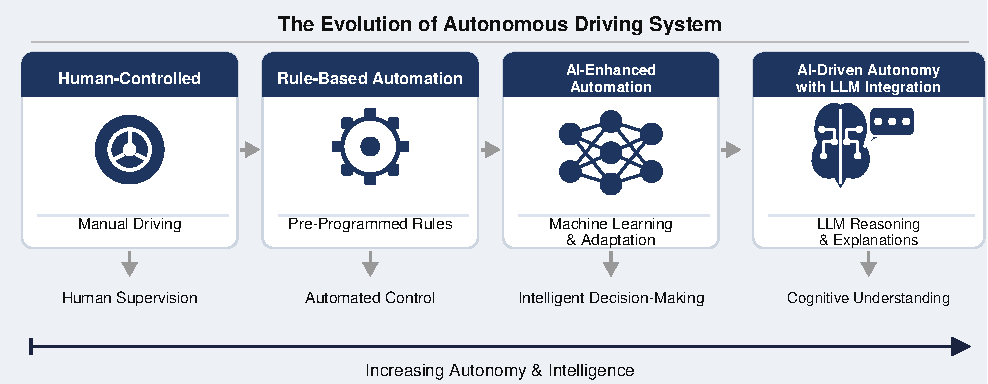
\includegraphics[width=0.7\textwidth]{Images/CH_1/flowchart_vector_cropped.pdf}
    % Figure 1.1 placeholder
    \caption{The Evolution of Autonomous Driving Intelligence: From Human Controlled Manual Driving to AI Driven Autonomy with LLM Integration.}
    \label{fig:1.1}
\end{figure}
The historical progression of autonomous vehicle research has been shaped by major milestones, including early academic demonstrations in the 1980s, the DARPA Grand Challenge \cite{thrun2006stanley}  and Urban Challenge competitions , and subsequent commercialization efforts by industry leaders \cite{urmson2008autonomous}. These milestones, illustrated in Figure \ref{fig:1.2} that presents a structured timeline of this technological evolution, highlighting how advances in sensing, computation, and artificial intelligence have progressively strengthened system capability and reliability. Contemporary autonomous driving systems are typically organized around a modular architecture consisting of perception, planning, and control components \cite{pendleton2017perception}. The perception module interprets sensor data from cameras, LiDAR, radar, GNSS, and inertial measurement units to construct an environmental representation. The planning module generates safe and efficient trajectories based on this representation, while the control module executes these trajectories through steering, acceleration, and braking commands. Although this modular framework has enabled scalable system development, it also introduces structural separation between environmental interpretation and motion execution.
\begin{figure}[h]
    \centering
    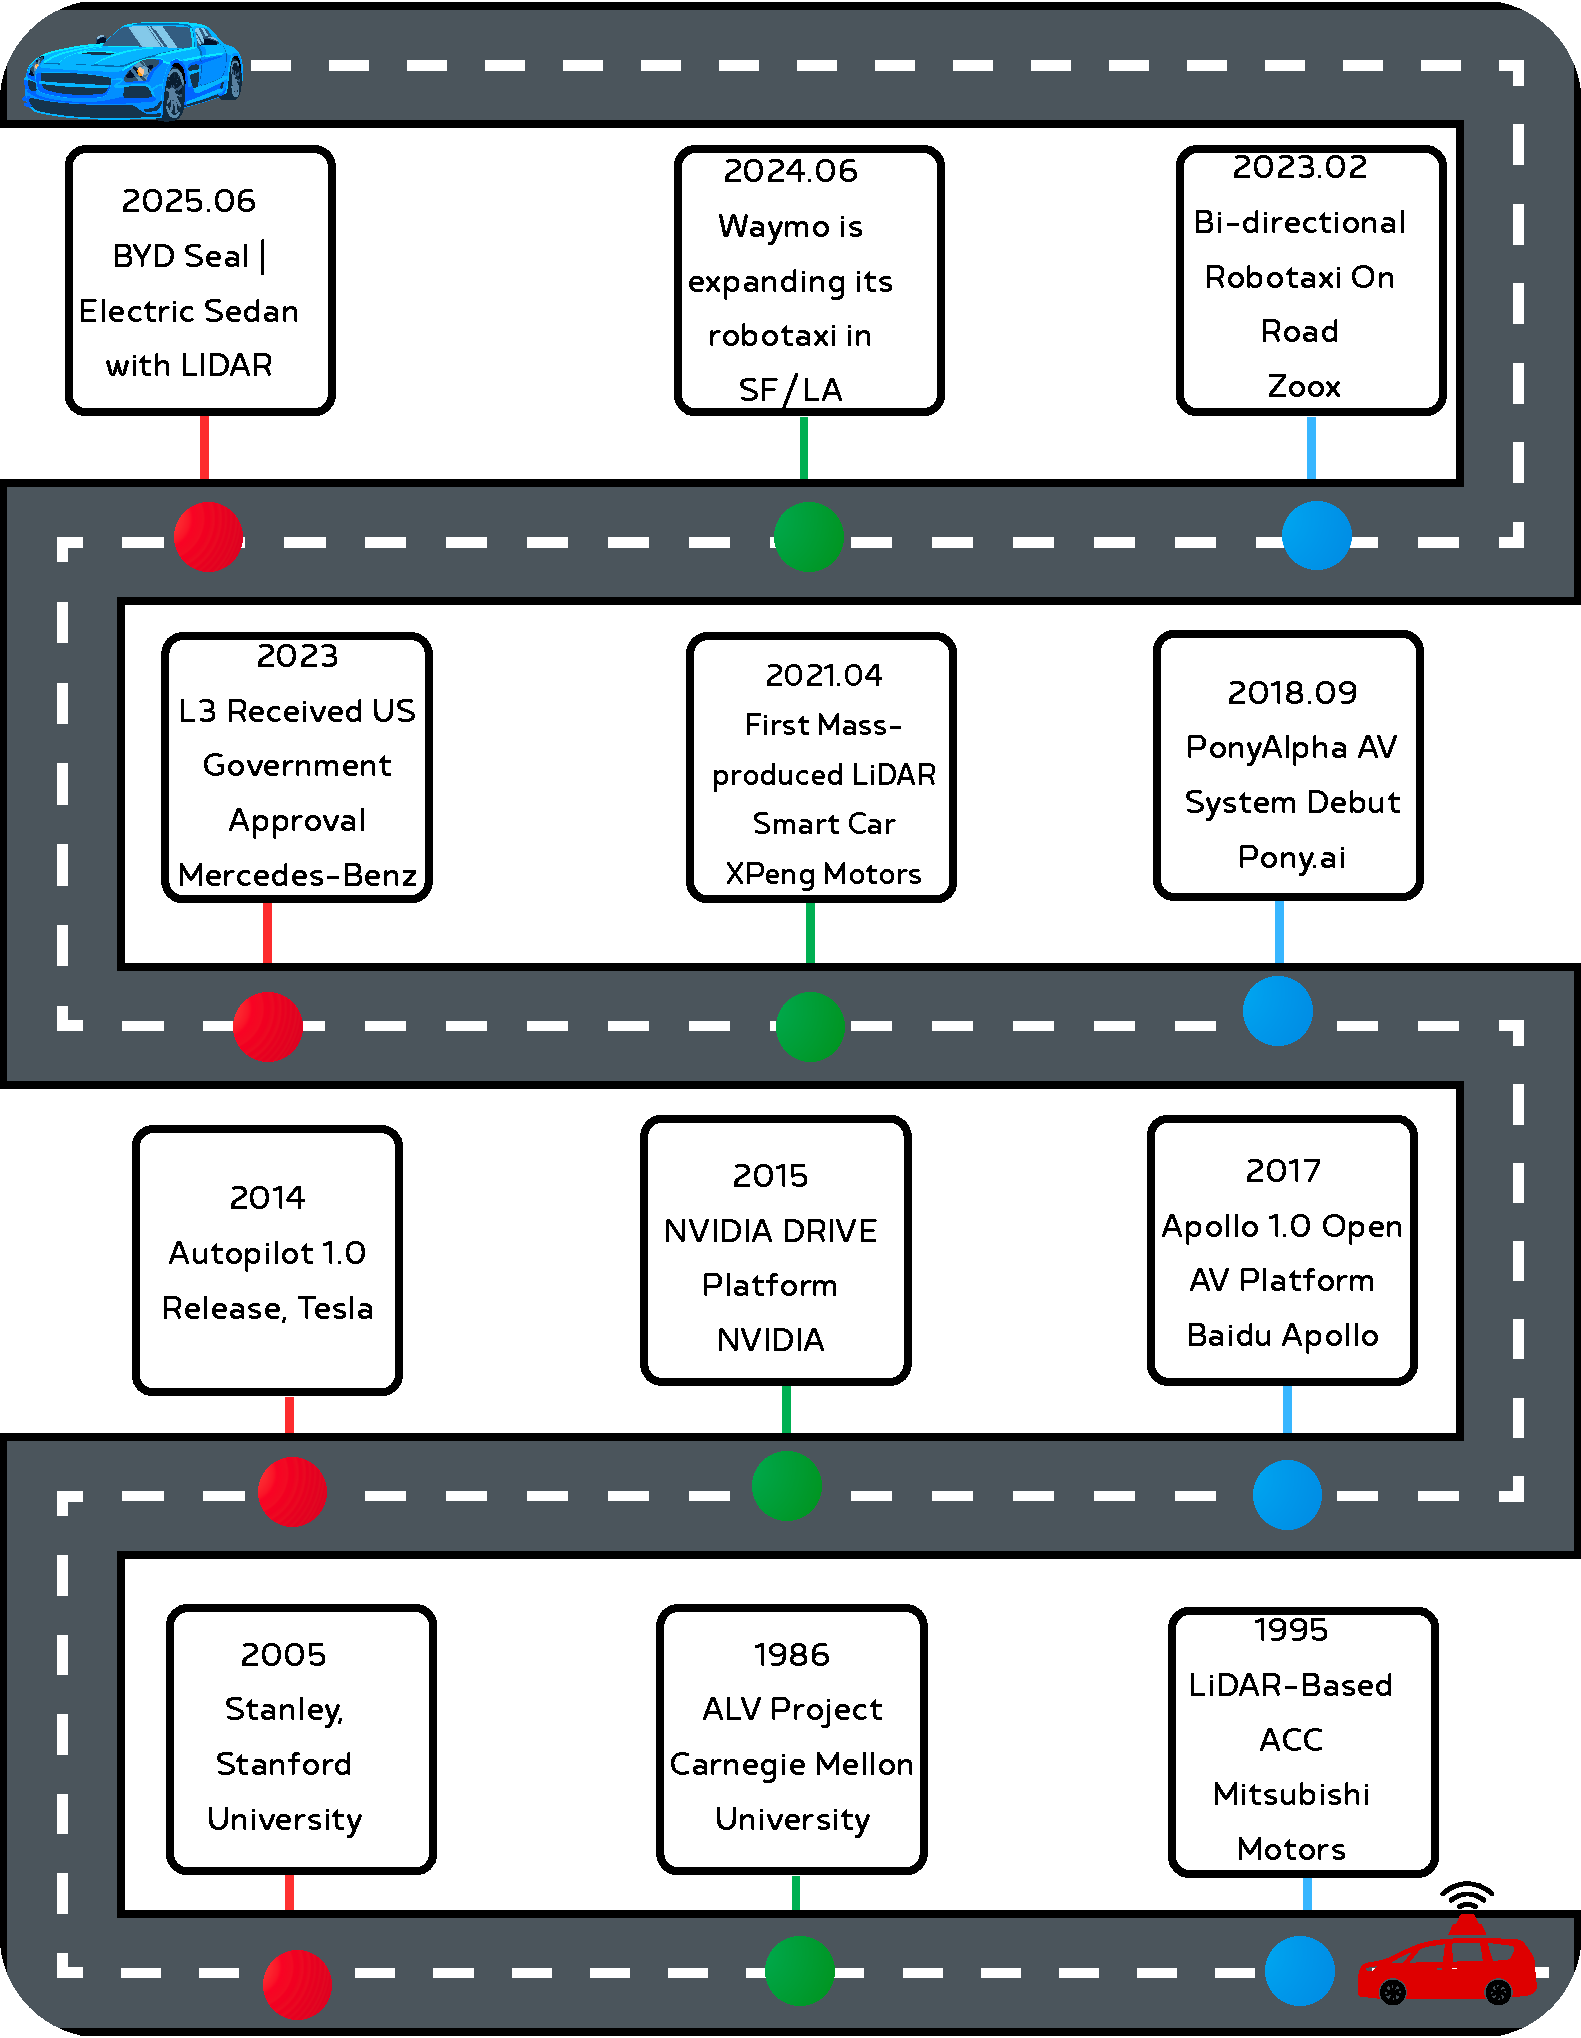
\includegraphics[width=0.7\textwidth]{Images/CH_1/History.pdf}
    % Figure 1.2 placeholder
    \caption{Tracking the journey of autonomous vehicles through major technological developments, including robotaxis, smart cars, and government approvals.}
    \label{fig:1.2}
\end{figure}
Recent advances in machine learning and deep learning have substantially improved perception accuracy and predictive modeling. However, increased reliance on data driven components has introduced new challenges related to interpretability and system transparency \cite{arrieta2020explainable}. In parallel, deterministic planning methods provide structured solutions with mathematical guarantees but often face computational constraints in complex driving scenarios. Furthermore, traditional system design primarily emphasizes collision avoidance and trajectory feasibility, while secondary performance factors such as ride comfort and infrastructure interaction receive comparatively limited integration.

\section{Limitations of Conventional Autonomous Driving Architectures}
Despite substantial progress in autonomous vehicle technology, current system architectures continue to exhibit inherent structural and operational constraints \cite{waymo2017road}. Most modern platforms adopt a modular perception planning control framework, where environmental sensing, trajectory generation, and motion execution are treated as sequential and largely independent processes. While this design facilitates engineering development and testing, it also introduces fragmentation in decision making. Information errors or uncertainties at the perception stage can propagate through the pipeline, affecting planning reliability and control stability.
Planning methodologies further reflect a persistent trade off between computational efficiency and path optimality. Graph based algorithms such as A* provide deterministic and structured solutions but may become computationally intensive in complex or high dimensional environments \cite{guruji2016time}. Sampling based approaches such as RRT offer flexibility and scalability; however, they often produce inconsistent convergence behavior and suboptimal trajectories in structured road scenarios. Achieving both real time performance and consistent path quality remains a practical challenge.
In parallel, the integration of data driven learning models has enhanced perception and prediction capabilities, yet it has also reduced system transparency \cite{tekkesinoglu2025advancing}. Many intelligent components function as opaque models with limited interpretability. In safety critical applications such as autonomous driving, the absence of explainable reasoning mechanisms complicates validation, debugging, and regulatory acceptance \cite{corso2020interpretable}.
Moreover, existing frameworks primarily emphasize safety and feasibility, often treating ride comfort and vehicle infrastructure interaction as secondary considerations \cite{fernandez2021trustworthy}. Dynamic responses to traffic calming structures, for example, are typically addressed at lower control layers rather than incorporated into high level planning strategies. This separation restricts the development of autonomous systems that balance safety, efficiency, and passenger comfort in an integrated manner.
Collectively, these limitations highlight the need for a cohesive framework that improves computational efficiency, enhances reasoning transparency, and integrates dynamic comfort considerations within a unified autonomous driving architecture.
\section{Research Motivation}
The limitations identified in conventional autonomous driving architectures indicate that further advancement requires more than incremental algorithmic improvements. As autonomous vehicles transition from controlled testing environments to complex real world deployment, system requirements extend beyond basic navigation and obstacle avoidance. Robust operation must be accompanied by computational efficiency, transparent decision making, and consistent dynamic performance.
The persistent trade off between structured path optimality and sampling based flexibility motivates the exploration of hybrid planning strategies capable of leveraging the strengths of both paradigms. An effective planning framework must ensure reliable convergence, maintain path quality, and operate within real time computational constraints. Addressing this balance is essential for scalable deployment in structured road networks.
Simultaneously, the increasing integration of learning based components raises important considerations regarding interpretability. In safety critical systems, decisions must not only be correct but also understandable. Transparent reasoning mechanisms can enhance system validation, facilitate debugging, and strengthen user and regulatory confidence. Incorporating advisory level intelligence while preserving deterministic control stability represents a meaningful step toward more accountable autonomous systems.
In addition to computational and cognitive aspects, dynamic interaction between the vehicle and roadway infrastructure remains an important yet under integrated dimension of autonomous mobility. Passenger comfort, particularly during traversal of traffic calming structures, is influenced by vehicle dynamics, geometric design, and speed regulation. Integrating comfort aware considerations within planning and control strategies can contribute to a more comprehensive performance framework.
These motivations collectively support the development of an integrated approach that enhances planning efficiency, introduces interpretable reasoning support, and incorporates dynamic comfort optimization within a unified autonomous driving architecture.
\section{Problem Statement}
Although autonomous driving technologies have progressed significantly, current architectures do not fully integrate computational efficiency, reasoning transparency, and dynamic comfort within a unified framework. Most systems rely on modular perception planning control pipelines that operate sequentially, often resulting in trade offs between real time responsiveness, trajectory optimality, and interpretability.
Planning algorithms typically favor either structured optimality or sampling flexibility, but seldom achieve both simultaneously under strict computational constraints. In parallel, the integration of intelligent reasoning components has improved contextual understanding; however, these mechanisms frequently operate as opaque models, limiting transparency in safety critical environments. To preserve control stability while enhancing interpretability, there is a need for an advisory level reasoning system that can provide structured decision support without directly overriding deterministic control processes.
Furthermore, vehicle infrastructure interactions, particularly those influencing ride comfort during traversal of traffic calming geometries, remain insufficiently incorporated into higher level planning strategies. Dynamic comfort considerations are commonly addressed at the control layer rather than integrated into planning and speed regulation decisions.
The central problem addressed in this thesis is therefore the development of an integrated autonomous driving framework capable of: Improving computational efficiency while maintaining trajectory quality. Enhancing interpretability through an advisory reasoning mechanism that supports but does not replace deterministic control, and Incorporating dynamic comfort considerations into motion planning and speed regulation.

Addressing these challenges requires a cohesive architectural approach that combines hybrid planning strategies, advisory level intelligent reasoning, and vehicle dynamic modeling within a practically implementable autonomous driving system.
\section{Research Objectives}
The primary objective of this research is to develop an integrated autonomous driving framework that improves planning efficiency, enhances reasoning transparency, and incorporates dynamic comfort considerations within a unified architecture. To achieve this goal, the thesis pursues the following specific objectives:
\begin{itemize}
\item To design and implement a hybrid path planning framework that combines structured search methods with sampling based strategies in order to balance trajectory optimality and computational efficiency under real time constraints.
\item To develop an advisory level reasoning mechanism capable of providing interpretable decision support without directly overriding deterministic control processes, thereby enhancing transparency while preserving system stability.
\item To model vehicle infrastructure interaction dynamics with particular emphasis on traffic calming geometries, enabling analytical evaluation of vertical acceleration and ride comfort metrics.
\item To derive geometry dependent safe traversal speed formulations that integrate dynamic response considerations into speed regulation strategies.
\item To validate the proposed framework through simulation based experimentation, including performance comparison with conventional approaches in terms of computational cost, trajectory quality, interpretability, and dynamic comfort.
\end{itemize}
Collectively, these objectives aim to establish a cohesive and practically implementable autonomous driving system that addresses efficiency, explainability, and passenger comfort within a single integrated structure.
\section{Research Contributions}
\begin{itemize}


\item A structured integration of deterministic graph based search and sampling based planning strategies is developed to improve computational performance while maintaining trajectory quality. The proposed hybrid formulation addresses the trade off between optimality and convergence behavior observed in conventional standalone approaches.
\item An interpretable advisory mechanism is introduced to provide contextual decision support without replacing deterministic control processes. By operating at an advisory layer, the framework enhances transparency and system explainability while preserving stability and safety critical reliability.
\item A geometry based analytical model is established to evaluate vehicle dynamic response during traversal of traffic calming structures. The formulation explicitly links speed breaker geometry to vertical acceleration characteristics and ride comfort metrics.
\item A geometry dependent safe speed formulation is derived based on dynamic response constraints, enabling the integration of comfort considerations into speed regulation strategies.
\item The proposed framework is validated through structured simulation experiments, including comparative performance evaluation against conventional planning and control approaches across metrics of computational cost, trajectory quality, interpretability, and dynamic comfort.

Together, these contributions demonstrate a unified architectural approach that extends beyond isolated algorithmic improvement, advancing the integration of efficiency, transparency, and comfort within autonomous vehicle systems.
\section{Organization of the Thesis}
Chapter 2 presents a comprehensive review of existing literature related to autonomous driving architectures, path planning methodologies, intelligent reasoning mechanisms, and vehicle infrastructure interaction modeling. The chapter establishes the theoretical foundation and identifies gaps addressed in this research. Chapter 3 describes the overall system architecture and integration framework, detailing the interaction between perception, planning, advisory reasoning, and control components.
Chapter 4 introduces the proposed hybrid path planning methodology and provides comparative performance evaluation against conventional approaches. Chapter 5 presents the advisory level reasoning mechanism, including its architectural design, operational structure, and evaluation within simulated driving scenarios. Chapter 6 develops the dynamic comfort modeling framework, including geometry based analysis of traffic calming structures and derivation of safe traversal speed formulations.
Finally, Chapter 7 summarizes the research findings, discusses limitations, and outlines potential directions for future work.

\newpage
     \chapter{Literature Review }
This chapter presents a comprehensive review of prior and related work underpinning the three research contributions of this thesis. The review is organized around three thematic pillars corresponding to the three studies: (1) Large Language Models in Autonomous Driving, (2) Path Planning Algorithms for Robot Navigation, and (3) Ride Comfort Optimization and Speed Breaker Design. Each section examines foundational methods, recent advances, identified gaps, and the motivations that guided the design choices in this thesis.
\section{Large Language Models in Autonomous Driving}
The integration of Large Language Models (LLMs) into autonomous driving systems has recently emerged as a promising direction for enhancing high level reasoning, contextual understanding, explainability, and personalization. Unlike traditional rule based or purely perception driven pipelines, LLM based frameworks attempt to incorporate semantic reasoning into driving decisions, enabling vehicles to interpret instructions, analyze scenarios, and generate human understandable explanations.As shown in Figure \ref{fig:2.1}
The study Cui et al\cite{cui2024receive} investigates the use of prompting strategies, including standard prompting and chain of thought reasoning, to improve driving decisions within simulation environments. The authors demonstrate that structured reasoning significantly enhances decision consistency. However, the framework relies on textual representations of the environment and lacks direct grounding in raw sensory perception, limiting real world deployment capability.
\begin{figure}[h]
    \centering
    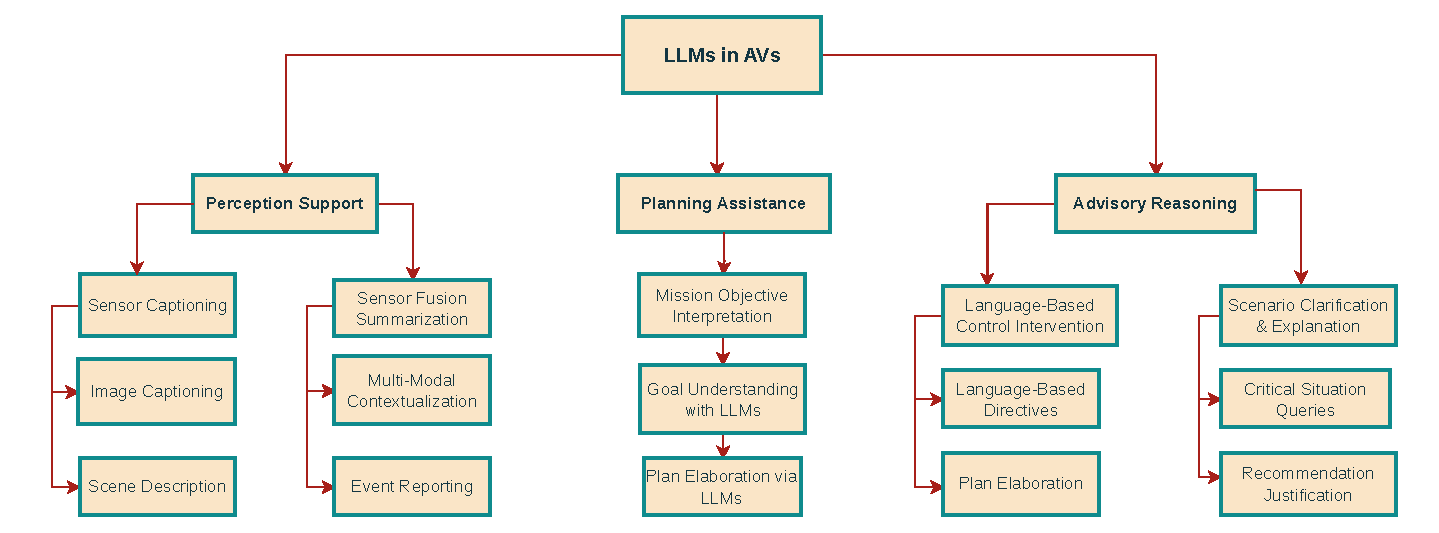
\includegraphics[width=0.9\textwidth]{Images/CH_2/LLM_in_Avs.pdf}
    % Figure 2.1 placeholder
    \caption{Overview of LLM integration in Autonomous Vehicles, categorized into Perception Support, Planning Assistance, and Advisory Reasoning, each encompassing specialized sub functions.}
    \label{fig:2.1}
\end{figure}
To address the grounding limitation, Chen et al \cite{chen2024driving} proposes aligning numeric object level vector representations with LLMs. By fusing structured numerical data with language reasoning, the system improves contextual understanding and explainability. Nevertheless, real time closed loop evaluation reveals computational and latency constraints, indicating that scalability remains a challenge.
Retrieval Augmented Generation (RAG) has been introduced to enhance contextual awareness in LLM based autonomous systems. Luo et al \cite{luo2025senserag} proposes a proactive retrieval framework that integrates multimodal sensor data and Vehicle to Everything (V2X) information into dynamically constructed knowledge bases. By enabling active querying of environmental data, the system enhances reasoning depth and contextual alignment. However, performance remains dependent on retrieval quality and indexing efficiency, particularly in real time scenarios. Personalization is explored in  Cui et al.\cite{cui2024personalized} through the Talk2Drive system, which enables vehicles to interpret natural language commands and store user preferences in memory modules. The study demonstrates reduced human intervention and improved user interaction. However, latency and memory management remain critical challenges when integrating personalization with safety critical control tasks.
Beyond operational driving tasks, V Zolfaghari et al. \cite{zolfaghari2024adopting} evaluates retrieval enhanced LLM frameworks in vehicle design applications. The study compares multiple LLMs, including GPT-4, LLaMA3, Mistral, and Mixtral, and confirms that RAG improves contextual accuracy and response relevance. Although focused on design support rather than real time driving, the work reinforces the broader applicability of retrieval enhanced reasoning in vehicle related domains.
Recent work by Liu et al. \cite{liu2025x} introduced X-Driver, which combines vision language models with chain of thought reasoning to support decision making in complex scenarios. The model generates step by step natural language rationale before issuing control commands, improving both interpretability and reliability. Wang et al. \cite{wang2025corra} developed CORRA, a system that leverages LLMs alongside model predictive control (MPC) for dynamic obstacle avoidance, demonstrating improved safety margins in cluttered environments. Wang et al. \cite{wang2023empowering} further showed that LLMs can act as high level decision makers alongside safety verifiers and trajectory planners, with behavior planning interacting with a predictor to make intelligent decisions especially where conventional deep neural networks struggle. Lu et al. \cite{lu2025convoyllm} introduced ConvoyLLM to coordinate multi lane convoy driving in dynamic environments, using LLMs to manage inter vehicle communication and lane change negotiations. Xu et al. \cite{xu2024drivegpt4} presented DriveGPT4, a multimodal framework capable of processing camera images and text simultaneously to explain vehicle decisions in natural language. Together, these works highlight that integrating LLMs with planning and control modules can enhance safety, transparency, and adaptability in complex driving scenarios. Yang et al. \cite{yang2023llm4drive} provided a comprehensive survey on the use of LLMs for autonomous driving, categorizing applications across perception, prediction, planning, and control, and identifying critical gaps in real time deployment and safety assurance. Tekkesinoglu et al. \cite{tekkesinoglu2025advancing} conducted a comprehensive review of explainable autonomous vehicle systems, emphasizing the importance of providing interpretable outputs that support driver trust, particularly during transitions between manual and automated control. Kim et al. \cite{kim2023and} evaluated on road explanations in highly automated vehicles and found that timely, scenario appropriate explanations significantly improve driver confidence. Corso and Kochenderfer \cite{corso2020interpretable} proposed interpretable safety validation frameworks specifically designed for autonomous vehicles to ensure that model behaviors remain auditable and understandable.
These studies highlight the necessity for interpretable and explainable models in autonomous driving. In response, this thesis proposes the Driving Transition Advisory System (DTAS), which addresses these gaps by delivering concise, real time LLM generated advisories without disrupting the core vehicle control pipeline.
\begin{figure}[h]
    \centering
    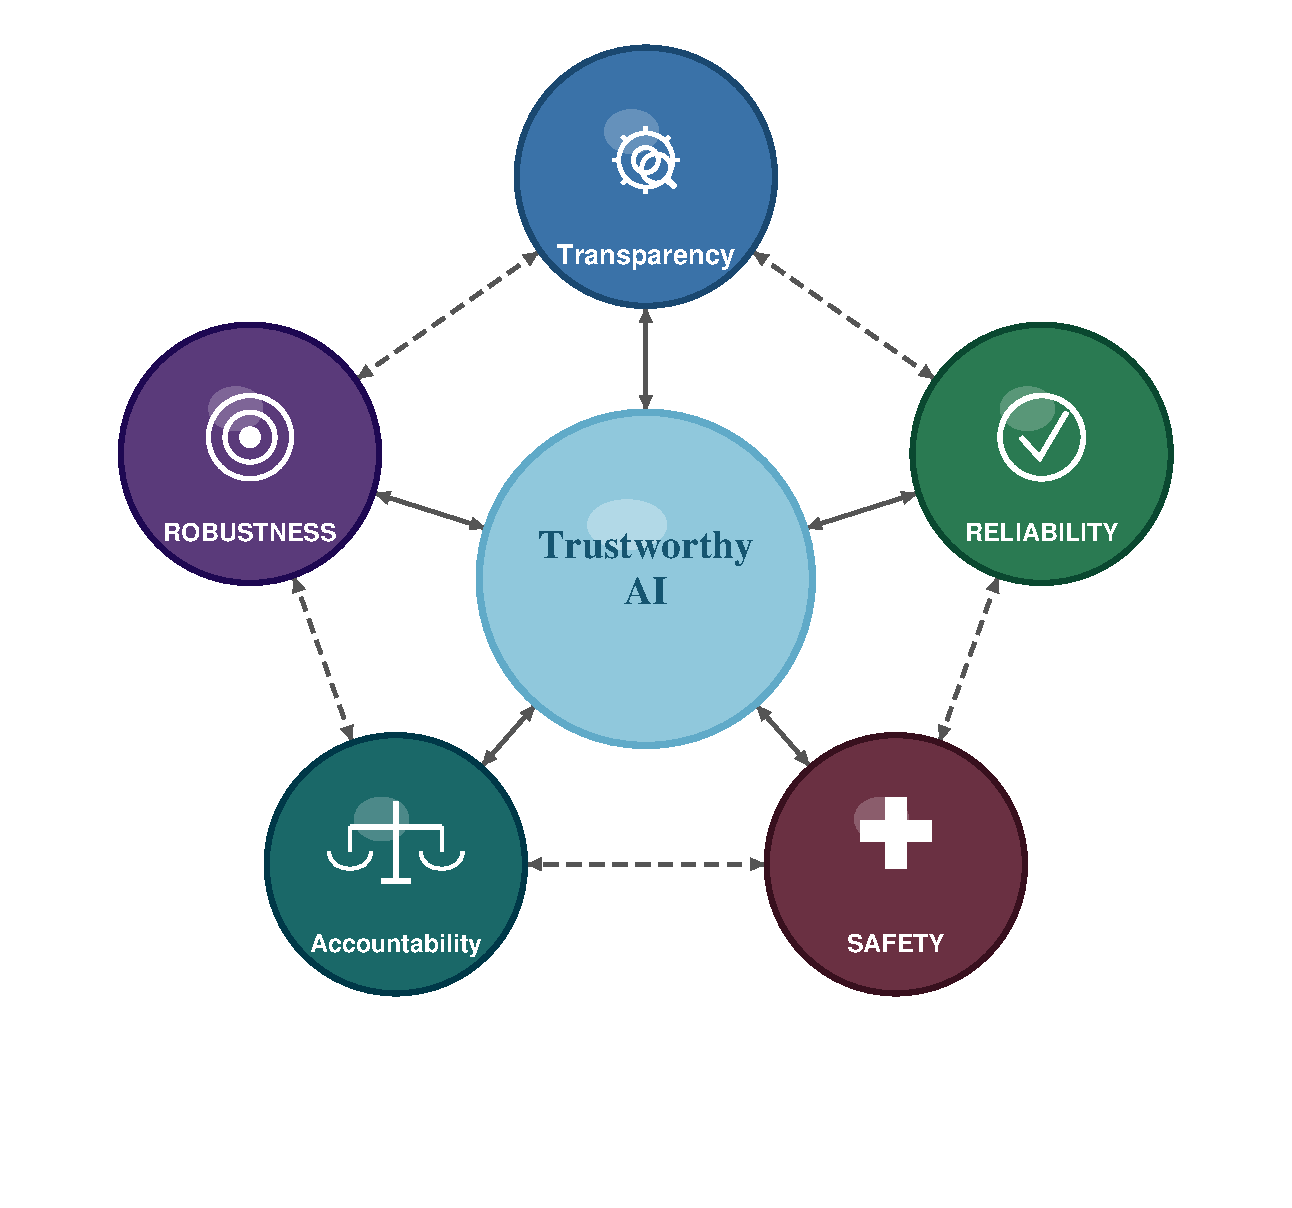
\includegraphics[width=0.65\textwidth]{Images/CH_2/trustworthy_ai.pdf}
    % Figure 2.2 placeholder
    \caption{presents the key principles of Trustworthy AI, including transparency, reliability, robustness, accountability, and safety, which together support responsible and secure AI deployment in safety critical systems.}
    \label{fig:2.2}
\end{figure}
As shown in Figure \ref{fig:2.2}, the principles of trustworthy AI transparency, reliability, safety, robustness, and accountability are crucial for ensuring the safety and reliability of autonomous systems. Arrieta et al. \cite{arrieta2020explainable} emphasize the importance of transparency in fostering user trust by providing clear reasoning behind system decisions. Schneiderman \cite{shneiderman2020human} highlights reliability, stressing the need for AI systems to perform consistently and accurately. Additionally, robustness ensures the system can handle unexpected conditions, while accountability ensures systems are designed with proper risk mitigation measures, as outlined by Schneiderman \cite{shneiderman2020human}.
While LLMs have the potential to enhance reasoning, explainability, personalization, and adaptability in autonomous systems, challenges persist in areas such as perception grounding, real time performance, retrieval optimization, and safe closed loop deployment. These challenges highlight the need for integrated frameworks that combine perception aware retrieval mechanisms with computationally efficient reasoning architectures, suitable for safety critical driving environments. This thesis addresses these challenges through the Driving Transition Advisory System (DTAS).
In the context of autonomous driving, explainability is essential for ensuring that system decisions are transparent and trusted by human operators. As black box models, which offer limited interpretability, are gradually replaced by more interpretable models, the need for transparent decision making logic grows. With advancements in autonomous systems, explainable and context aware advisory systems are becoming indispensable for clarifying driving decisions in real time. This transition is visualized in the spectrum of explainability shown in Figure \ref{fig:2.3}.
\begin{figure}[h]
    \centering
    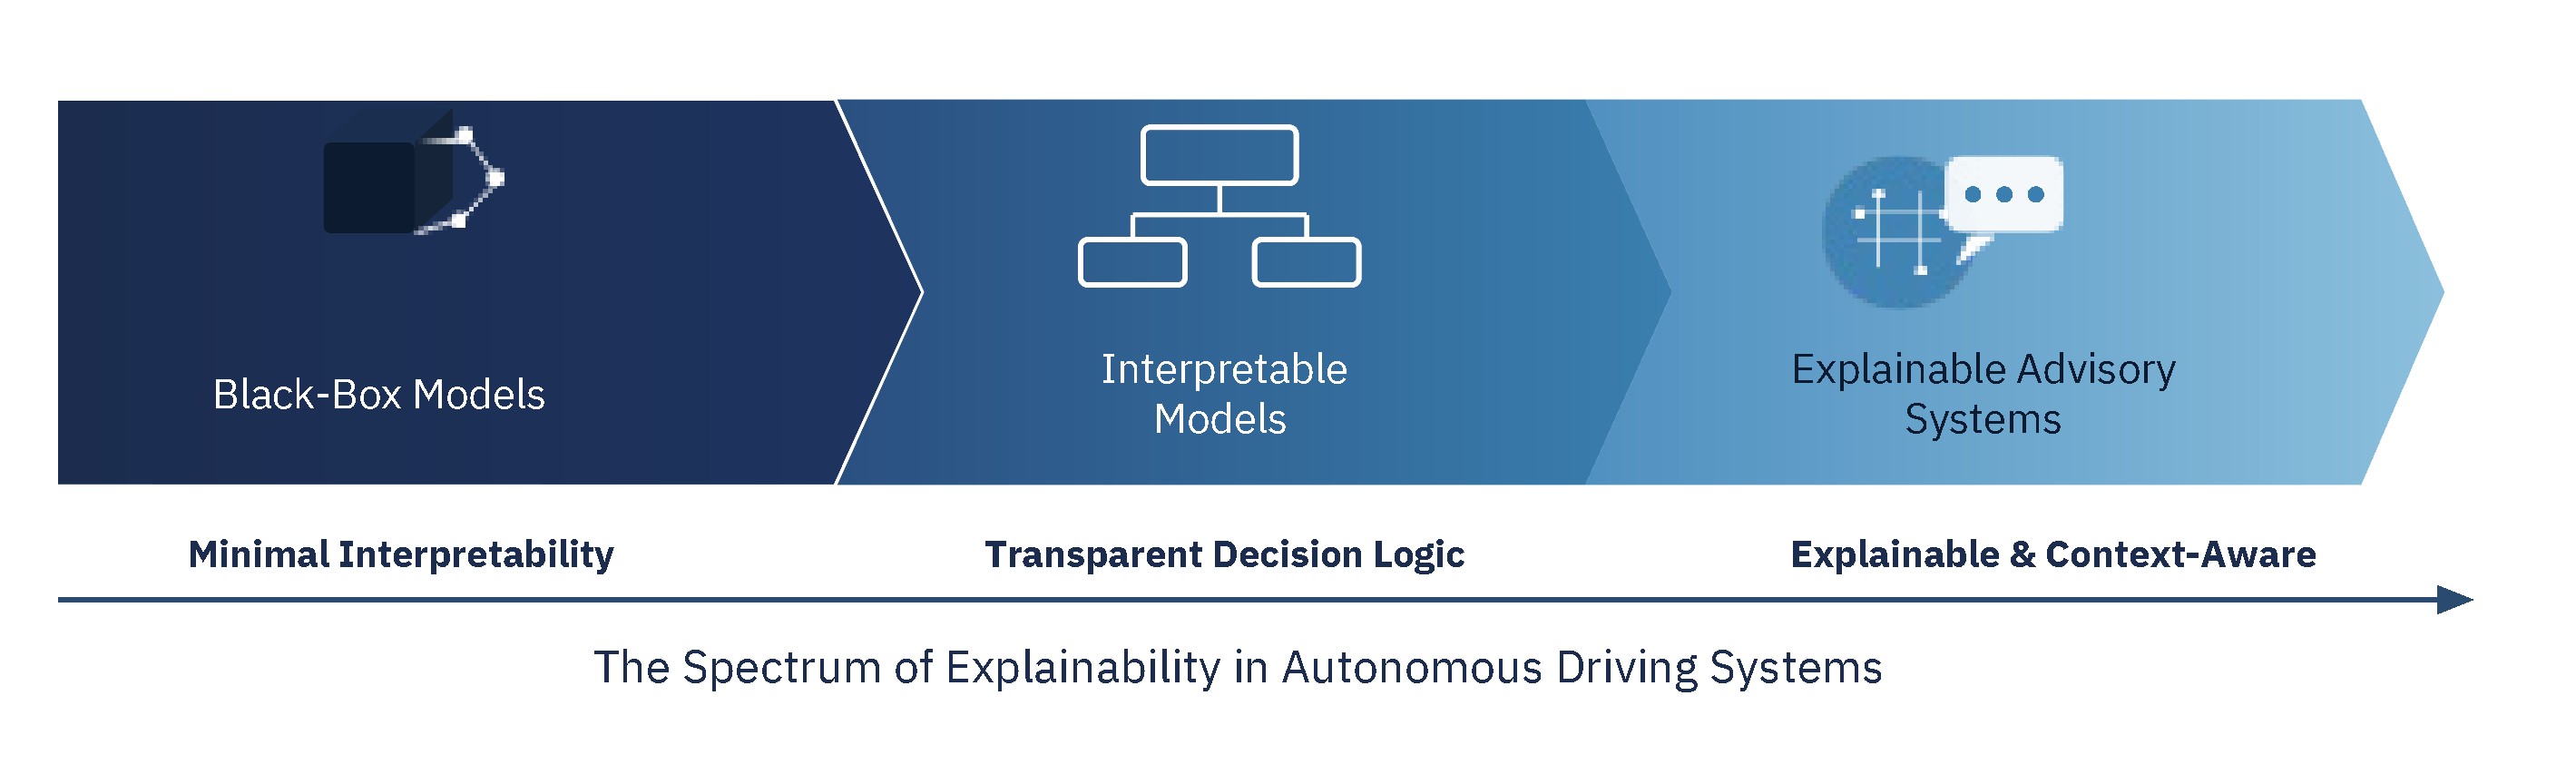
\includegraphics[width=0.9\textwidth]{Images/CH_2/spec.pdf}
    % Figure 2.3 placeholder
    \caption{The spectrum of explainability in autonomous driving systems, progressing from opaque black box models through interpretable models to fully explainable and context aware advisory systems.}
    \label{fig:2.3}
\end{figure}
\section{Path Planning Algorithms for Robot Navigation}
Path planning is fundamental to autonomous system navigation, serving as the foundation for computing collision free paths that are both safe and efficient. The primary challenge lies in designing algorithms capable of computing feasible paths quickly while avoiding obstacles and reaching the destination optimally. An effective path planning algorithm must balance multiple considerations: computational speed, real time responsiveness, and robustness in real world situations. The evolution of path planning has progressed from heuristic based methods such as A* to sampling based approaches like RRT and its variants.
\subsection{Heuristic Based Planning: A* and Variants}
The A* algorithm  remains a foundational benchmark in grid based path planning due to its optimality guarantees when using an admissible heuristic. Defined by the cost function F(n) = g(n) + h(n), where g(n) is the actual cost from start to node n and h(n) is a heuristic estimate to the goal, A* systematically explores the state space and guarantees the shortest path. Guruji et al. \cite{guruji2016time} proposed a time efficient A* implementation suitable for robotic path planning, demonstrating significantly reduced computation time through improved priority queue management. Ju et al. \cite{ju2020path} further enhanced A* using adaptive heuristic weighting to reduce unnecessary node expansions in complex structured environments. Despite these improvements, A* scales poorly to high dimensional or unstructured spaces where the grid resolution creates exponential node growth, as documented by Souissi et al. \cite{souissi2013path}.
\section{Sampling Based Planning: RRT and RRT*}
Sampling based methods were introduced to overcome the curse of dimensionality inherent in grid based approaches. Rapidly exploring Random Trees (RRT) \cite{lavalle2001randomized} probabilistically construct search trees by sampling random configurations in the free configuration space, ensuring probabilistic completeness without exhaustive node expansion. RRT* extended this to asymptotic optimality through a rewiring process that iteratively refines the tree as new samples are added, yielding near optimal paths with sufficient iterations. Nasir et al. \cite{nasir2013adaptive} proposed adaptive RRT* Smart, which accelerates convergence by biasing sampling toward collision free regions already explored. Islam et al. \cite{islam2012rrt} demonstrated that RRT* Smart achieves significantly faster convergence than standard RRT* in cluttered environments. However, slow convergence and stochastic path quality remain persistent limitations of purely sampling based approaches, particularly when deterministic path quality is required.A comparison between A* and RRT* Algorithm is mentioned in Figure \ref{fig:2.4}
\begin{figure}[h]
    \centering
    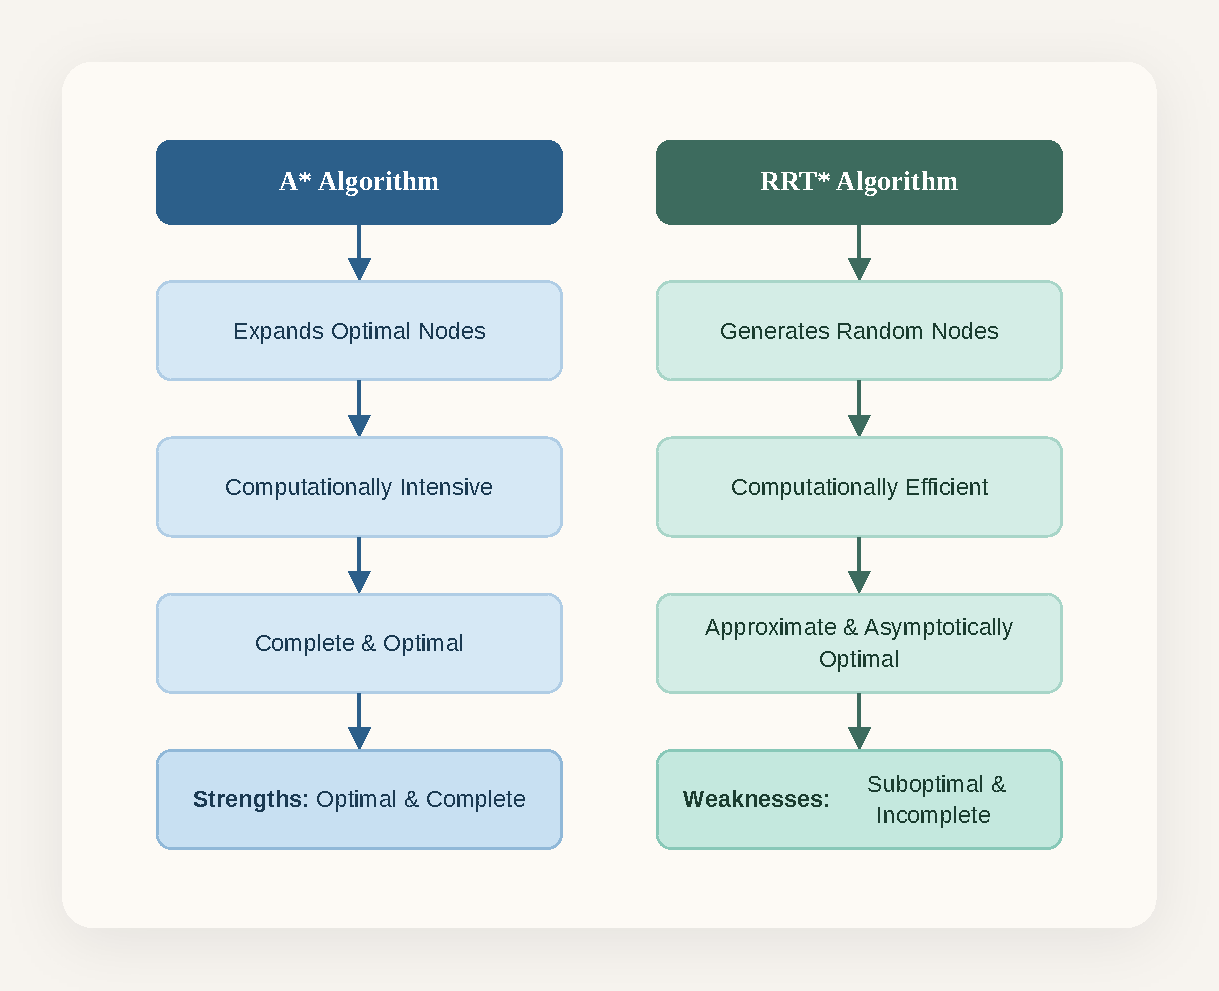
\includegraphics[width=0.7\textwidth]{Images/CH_2/algorithm_comparison.pdf}
    % Figure 2.4 placeholder
    \caption{A comparison between A* and RRT* path planning algorithms, where A* guarantees an optimal and complete solution but is computationally heavy, while RRT* is faster but may produce suboptimal results.}
    \label{fig:2.4}
\end{figure}
\section{Hybrid Planning Approaches}
To address the complementary limitations of A* and RRT*, researchers have explored hybrid frameworks that combine heuristic driven accuracy with probabilistic exploration. Brennan et al. \cite{brennan2024comparative} conducted a systematic comparison of A* and RRT* across four maze environments, including single solution, ladder, high density, and low density obstacle layouts. Their findings indicate that A* is computationally faster (3–5 times) in structured grids but struggles in complex or open environments, while RRT* produces smoother paths at a higher computational cost.
Ansarry et al.\cite{al2021hybrid} proposed Hybrid RRT-A*, which integrates the heuristic guidance of A* into the tree expansion strategy of RRT to reduce convergence time and improve path quality in cluttered environments. In the worst case, Hybrid RRT-A* discovered a route in 4.9 seconds, compared to 18.3 seconds for A* and 34 seconds for RRT, a substantial improvement that validates the hybrid strategy. Mashayekhi et al. \cite{mashayekhi2020hybrid} further proposed Hybrid RRT, a semi dual tree motion planner that improves exploration efficiency through bidirectional tree growth.
Ganesan et al. \cite{ganesan2024hybrid} presented a hybrid sampling based RRT* algorithm integrating uniform and non uniform sampling strategies. Tested against RRT*, Informed RRT*, and RRT* N, the hybrid approach achieved 76.9\% faster convergence, 48.53\% fewer nodes explored, and 44.02\% reduced planning time. These results validate the principle of combining complementary strengths deterministic heuristics with probabilistic exploration to achieve simultaneous gains in speed and path quality
Liao et al. \cite{liao2024research} proposed an integration of adaptive A* with the Dynamic Window Approach (DWA) for mobile robot navigation, demonstrating improved real time performance in dynamic environments. Kiani et al. \cite{kiani2021adapted} developed an adapted RRT hybrid for three dimensional path planning using metaheuristic sampling, addressing the challenges of 3D obstacle dense environments that extend beyond maze navigation.
Despite these advances, most hybrid methods have been evaluated in isolated test environments with fixed obstacle configurations. The systematic evaluation of hybrid planners across dynamically generated mazes with adjustable complexity remains underexplored. The Adaptive A* RRT* proposed in this work directly addresses this gap by introducing a tunable bias parameter $\lambda$ that allows practitioners to balance between deterministic and stochastic exploration depending on environment complexity.
\section{Ride Comfort Optimization and Speed Breaker Design}
Ride comfort represents a critical dimension of autonomous vehicle user experience that is distinct from safety or path optimality. As vehicles traverse road infrastructure such as speed breakers (road humps), the induced vertical accelerations and pitch motions directly affect passenger comfort. Engineering traffic calming devices and the vehicle's speed response to them presents a multidisciplinary challenge at the intersection of road geometry design, vehicle dynamics, and longitudinal control.
\subsection{Speed Breaker Geometry and Standards}
Traditional speed breaker designs, including flat top humps, sinusoidal profiles, and parabolic humps, have been studied extensively from the perspective of pedestrian safety and vehicle speed reduction. Federal Highway Administration (FHWA) \cite{ewing1999traffic} guidelines classify traffic calming devices by geometry, height, and intended speed reduction, providing a standardized framework for deployment. However, most standard profiles are not optimized for ride comfort, particularly for sensitive populations or high speed autonomous vehicles that must traverse without human anticipatory adjustment.
Raised cosine profiles have been proposed as smoother alternatives to conventional rectangular or sinusoidal humps. Darwish and Abu Bakar \cite{darwish2015traffic} studied traffic density estimation in the context of vehicular systems, showing that vehicle behavior in the vicinity of traffic calming elements is closely tied to local traffic density, a factor that adaptive speed controllers must incorporate. The raised cosine geometry, characterized by continuous first derivatives, produces gentler transitions that reduce impulsive forces on the vehicle suspension and improve passenger comfort.
\subsection{Vehicle Dynamics and Comfort Metrics}
The dynamics of a vehicle traversing a road hump are typically modeled using quarter car or half car models that capture vertical displacement, pitch angle, and suspension forces. Rokonuzzaman et al. \cite{rokonuzzaman2021model} demonstrated that Model Predictive Control (MPC) with learned vehicle dynamics significantly improves path tracking performance for autonomous vehicles, highlighting the importance of incorporating dynamic vehicle behavior into controller Pendleton et al. \cite{pendleton2017perception} provided a comprehensive framework for the perception, planning, control, and coordination modules of autonomous vehicles, emphasizing that longitudinal control must account for physical vehicle dynamics to ensure both safety and comfort.
\subsection{Adaptive Speed Control for Traffic Calming}
Adaptive speed control systems adjust vehicle velocity in anticipation of road features to minimize discomfort. Bennett [33] reviewed the development of PID controllers, which remain widely used for longitudinal velocity regulation due to their simplicity and robustness. However, conventional PID controllers operate reactively and lack the predictive capability needed to smoothly decelerate before a speed breaker and re accelerate afterward. MPC based approaches, as reviewed by Rokonuzzaman et al. \cite{rokonuzzaman2021model}, offer model based anticipation by optimizing control actions over a finite prediction horizon, making them better suited to smooth speed transitions around geometric road features.
Geisslinger et al. \cite{geisslinger2023ethical} proposed an ethical trajectory planning algorithm for autonomous vehicles that explicitly considers passenger comfort alongside safety constraints, framing ride quality as a first class objective rather than a secondary consideration. Llorca and Gomez \cite{fernandez2021trustworthy} emphasized that trustworthy autonomous vehicles must meet user expectations not only in terms of crash avoidance but also in terms of ride smoothness and predictability, particularly as public adoption depends on passenger confidence.
Despite these contributions, the specific challenge of integrating raised cosine speed breaker geometry with an adaptive longitudinal speed controller in a physics based co simulation environment as proposed in Chapter 6 of this thesis has received limited attention. Most existing work either focuses on static geometry optimization without dynamic vehicle response or designs speed controllers independently of road geometry. The approach taken in this thesis bridges these two dimensions in a unified CarSim-MATLAB framework.
\section{Autonomous Vehicle Simulation Environments}
Validated simulation environments are essential for testing autonomous vehicle algorithms safely and reproducibly. CARLA \cite{dosovitskiy2017carla} has become the de facto open source simulator for autonomous driving research, offering photorealistic rendering, configurable traffic scenarios, and integration with sensor suites including cameras, LiDAR, and GPS. Wen et al. \cite{wen2020scenario} proposed a scenario generation pipeline for AV simulators that enables systematic test case construction, supporting reproducibility in evaluation. The CARLA environment is used in Chapter 5 of this thesis to evaluate the Driving Transition Advisory System (DTAS) under realistic urban driving conditions.
For the path planning study in Chapter 4, a Python based maze environment with configurable grid cell sizes was developed, following the methodology of Brennan et al. \cite{brennan2024comparative}, which uses maze complexity as a systematic experimental variable. The CarSim-MATLAB co simulation platform provides high fidelity vehicle dynamics modeling for the ride comfort study in Chapter 6, offering validated suspension models and longitudinal dynamics that are essential for meaningful comfort evaluation.
The diversity of simulation platforms across the three studies reflects the specificity of each research question. A maze planner is best evaluated in a controlled graph search environment; an LLM advisory system requires a realistic urban traffic simulator; and a ride comfort framework demands a physics accurate vehicle dynamics model. 
\section{Summary and Research Gaps}
The literature reviewed in this chapter reveals several consistent patterns and persistent gaps that directly motivate the contributions of this thesis. First, while LLMs have demonstrated strong potential for reasoning and explanation generation in autonomous driving contexts, no existing framework integrates both Llama3 and Mistral in a modular, real time advisory system embedded within a conventional AV pipeline a gap addressed by the DTAS. Second, hybrid path planning algorithms have shown consistent advantages over pure A* and pure RRT*, yet systematic evaluation across dynamically generated environments with variable complexity and tunable bias parameters remains absent a gap addressed by the Adaptive A* RRT*. Third, although ride comfort has been recognized as a critical dimension of autonomous vehicle trustworthiness, the co design of raised cosine speed breaker geometry with an adaptive speed controller in a validated vehicle dynamics simulator has not been demonstrated.
Together, these three gaps define a coherent research agenda centered on the integration of intelligent augmentation strategies with conventional autonomous vehicle control architectures. The following chapter presents the unified research methodology that connects all three contributions into a single, cohesive thesis framework.
\newpage
     \chapter{RESEARCH METHODOLOGY AND SYSTEM DESIGN OVERVIEW}
\section{Problem Statement }
Autonomous vehicle \cite{wen2020scenario} systems primarily rely on conventional planning and control algorithms to ensure safe and efficient navigation. These algorithms, including deterministic path planning strategies and model based longitudinal and lateral controllers, are designed to optimize trajectory generation, stability, and constraint satisfaction under structured environmental conditions. Such conventional frameworks are mathematically grounded, computationally efficient, and suitable for safety critical applications. However, despite their robustness, they remain fundamentally limited in their ability to provide semantic reasoning, contextual interpretation, and understandable explanations of decision making processes.
In real world driving scenarios, especially under dynamic and uncertainty rich environments, the ability to interpret system behavior becomes increasingly important. While conventional controllers can determine when to slow down, avoid obstacles, or adjust trajectory curvature, they do not inherently communicate why such actions are executed. This lack of interpretability presents challenges in human machine interaction, trust calibration, and supervisory control contexts. Furthermore, deterministic control architectures are typically rule based or optimization driven, lacking higher level contextual reasoning capabilities that may assist in anticipating complex scenario transitions.
Recent advancements in Large Language Models (LLMs) have demonstrated significant capability in contextual understanding, reasoning, and natural language generation. Unlike conventional control systems, LLMs can process structured state information and generate semantically meaningful interpretations of system behavior. This capability introduces an opportunity to augment autonomous vehicle architectures with a cognitive reasoning layer that enhances transparency and interpretability without compromising safety critical execution.
The central problem addressed in this research is therefore defined as follows:
How can a Large Language Model be integrated with a conventional autonomous vehicle control framework in a manner that enhances contextual reasoning and interpretability while preserving the reliability, stability, and real time performance of deterministic control mechanisms?
To address this problem, the proposed approach does not seek to replace conventional planning and control algorithms. Instead, it aims to develop a non intrusive integration strategy in which the LLM operates as a parallel advisory module. The conventional control pipeline remains responsible for trajectory generation and actuation commands, while the LLM observes structured system states and produces high level reasoning outputs. This separation ensures that safety critical decisions remain deterministic, while cognitive augmentation is introduced at the advisory level.
The motivation behind this integration lies in bridging the gap between algorithmic control precision and human centered interpretability. By combining the mathematical rigor of conventional control with the contextual reasoning capability of LLMs, the proposed framework aspires to establish a layered autonomous system architecture that is both technically robust and cognitively transparent \cite{tekkesinoglu2025advancing}. Subsequent sections of this chapter describe the architectural components and integration strategy that enable this unified framework.
\section{Conventional Control Framework}
The foundation of the proposed system is a conventional autonomous driving control architecture composed of perception, planning, and control modules operating in a closed loop manner. As Shown in Figure \ref{fig:3.1}. This deterministic backbone is responsible for real time environment interpretation, trajectory generation, and vehicle actuation, ensuring safety, stability, and computational reliability under structured and semi structured driving conditions. At the perception level, environmental information is acquired through simulated sensor inputs, including object positions, traffic signal states, road geometry, and dynamic obstacle behavior. These inputs are processed to generate a structured representation of the driving scene, including lane boundaries, vehicle states, obstacle proximity, and contextual traffic indicators. The perception module transforms raw environmental data into state variables that can be utilized by higher level planning algorithms.
The planning layer operates on this structured state representation to generate feasible and collision free trajectories. In this research, a hybrid planning strategy based on Adaptive A* RRT* is employed to combine heuristic guided search with sampling based optimization. The deterministic component ensures efficient convergence toward goal directed trajectories, while adaptive sampling improves performance in constrained environments. 
\begin{figure}[h]
    \centering
    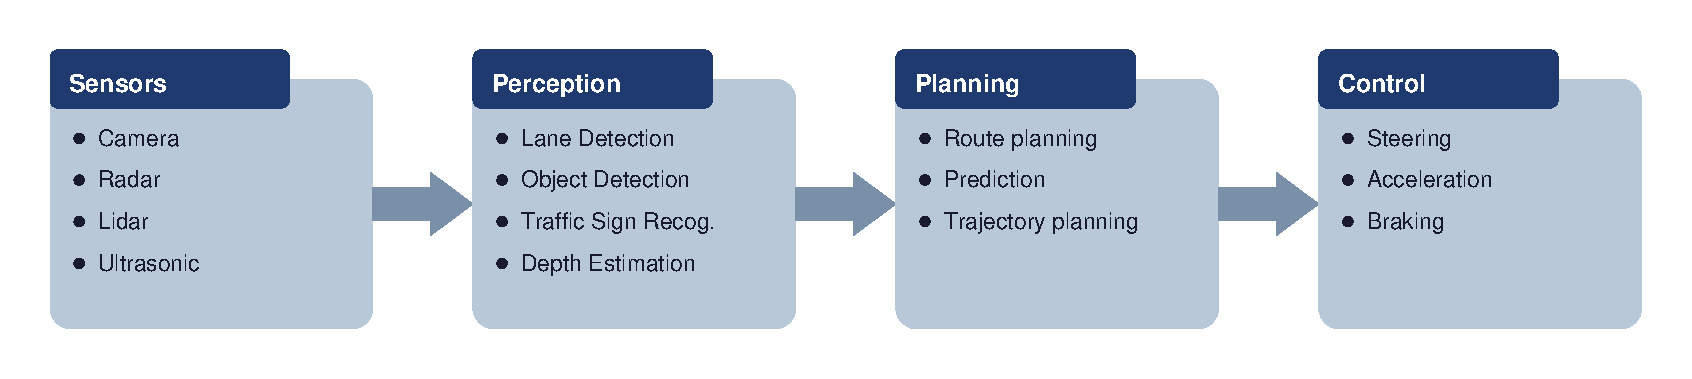
\includegraphics[width=0.8\textwidth]{Images/CH_3/pipeline_diagram (1).pdf}
    % Figure 3.1 placeholder
    \caption{Conceptual framework of an autonomous vehicle system, demonstrating the sequential interaction between sensors, perception, planning, and control layers.}
    \label{fig:3.1}
\end{figure}
The planning module outputs a reference trajectory defined in spatial and temporal coordinates, satisfying kinematic and environmental constraints.
Following trajectory generation, the control module translates the planned path into executable vehicle commands. Longitudinal and lateral controllers regulate throttle, braking, and steering inputs to track the reference trajectory while maintaining dynamic stability. The longitudinal controller governs velocity adaptation according to environmental conditions, while the lateral controller ensures accurate path tracking and lane alignment. These controllers operate under predefined stability and safety constraints, guaranteeing predictable vehicle behavior.
The conventional framework is inherently deterministic and mathematically grounded. It optimizes trajectory smoothness, minimizes control effort, and satisfies safety margins using structured optimization techniques. However, while it achieves high performance in trajectory execution and stability control, it lacks semantic reasoning capability. The system can compute optimal actions, but it does not provide contextual explanations or high level interpretations of its decisions.
This deterministic architecture serves as the safety critical core of the proposed research. It establishes baseline performance for navigation and control and ensures that real time actuation remains independent of non deterministic reasoning modules. The subsequent sections introduce the LLM based advisory component and describe how it is integrated with this conventional backbone without interfering with safety critical control execution.
\section{LLM Based Advisory Module}
The conceptual role of the LLM \cite{yang2023llm4drive} advisory layer within the autonomous driving framework is illustrated in Figure \ref{fig:3.2}. The model operates in parallel with the deterministic control module, observing structured vehicle states and generating contextual reasoning outputs without influencing physical actuation commands. This layered separation forms the foundation of the proposed cognitive augmentation strategy. While the conventional control framework ensures reliable and deterministic vehicle operation, it does not inherently provide contextual reasoning or human understandable interpretation of its actions.

\begin{figure}[h]
    \centering
    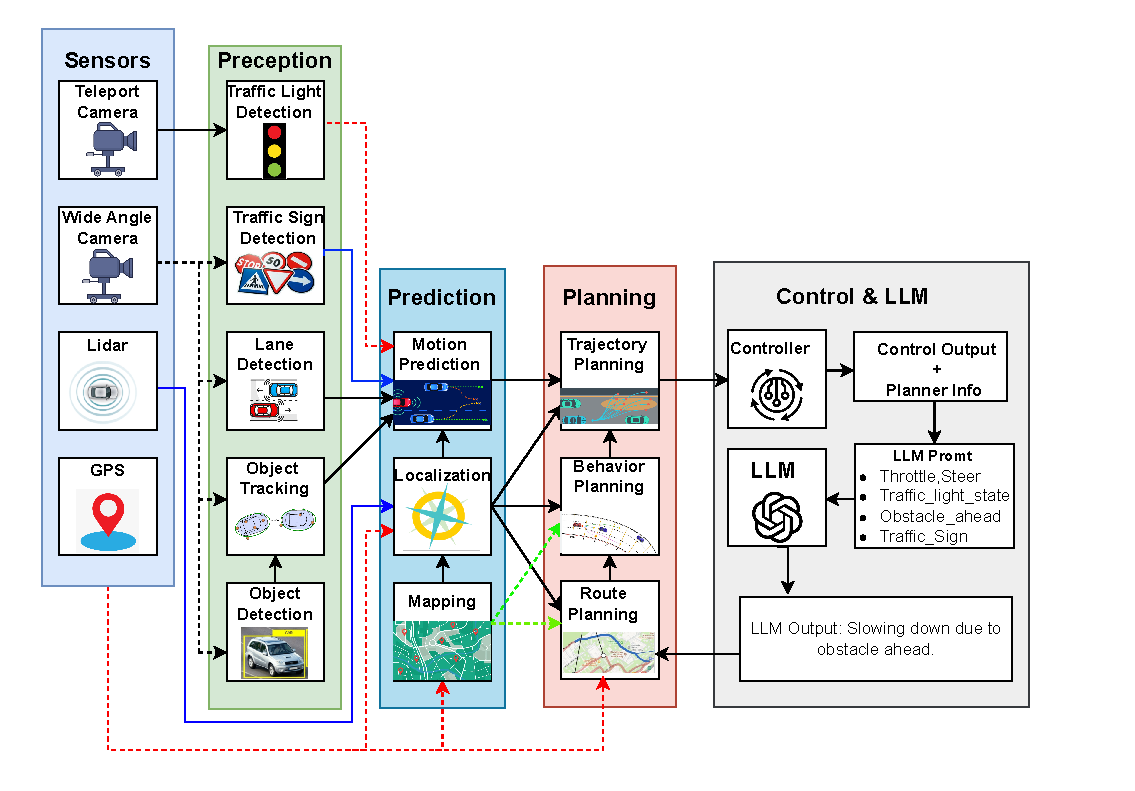
\includegraphics[width=0.9\textwidth]{Images/CH_3/Methodology.pdf}
    % Figure 3.3 placeholder
    \caption{End-to-end autonomous driving pipeline integrating sensing, perception, prediction, planning, control, and LLM based decision explanation within a unified framework.}
    \label{fig:3.2}
\end{figure}
To address this limitation, a Large Language Model (LLM) based advisory module is introduced as a parallel cognitive layer within the proposed architecture.
The LLM module is designed to observe structured system states generated by the perception and planning layers. These states include vehicle speed, trajectory curvature, obstacle proximity, traffic signal conditions, lane information, and environmental constraints. Rather than directly influencing actuation commands, the LLM processes this structured data and generates high level semantic outputs that describe the reasoning behind the vehicle’s behavior.
The advisory module operates through a structured state to text transformation mechanism. Relevant system parameters are formatted into standardized prompts that encode the current driving context. These prompts are then provided to LLM, which generates context aware explanations or advisory messages. For example, in scenarios involving obstacle avoidance or speed reduction near road disturbances, the LLM can articulate the rationale behind deceleration or trajectory modification in natural language form.
The primary objective of this module is not to replace conventional control algorithms, but to augment the system with cognitive transparency. By introducing semantic reasoning, the LLM enhances interpretability, supports supervisory understanding, and contributes to improved human machine interaction. This capability is particularly relevant in semi autonomous systems where driver transition awareness and system trust calibration are critical.
To ensure safety and stability, the LLM module is implemented as a non intrusive advisory layer. It does not modify control signals, override trajectory decisions, or directly influence vehicle actuation. Instead, it operates asynchronously alongside the conventional pipeline, observing system states and generating explanatory outputs. This separation preserves the deterministic nature of safety critical control operations while enabling contextual reasoning at a higher abstraction level.
Additionally, latency management mechanisms are incorporated to ensure that LLM inference does not interfere with real time control loops. The advisory outputs are generated within acceptable computational constraints, and fallback strategies are maintained to guarantee uninterrupted control execution in the event of delayed or unavailable LLM responses.
Through this architecture, the proposed system establishes a layered structure in which deterministic control ensures physical safety and stability, while the LLM module contributes interpretability and contextual intelligence. The next section details the integration mechanism that governs data exchange and operational coordination between these components.
\section{Integration Mechanism}
The integration of the Large Language Model with the conventional control framework is designed to ensure cognitive augmentation without compromising safety critical operation. The proposed mechanism follows a non intrusive, parallel architecture in which deterministic planning and control remain the primary decision making authority, while the LLM operates as an observational and advisory layer.
\subsection{Parallel Integration Architecture}
In the proposed system, the conventional pipeline consisting of perception, planning, and control executes in a closed loop configuration responsible for trajectory generation and actuation commands. The LLM module is connected to this pipeline through a structured state monitoring interface. Instead of modifying control outputs, the LLM observes selected system variables such as vehicle speed, planned trajectory characteristics, obstacle proximity, and environmental context.
This parallel configuration ensures that:
Control commands are always generated by deterministic algorithms. The LLM does not inject or override actuation signals. Safety and stability remain independent of non deterministic reasoning.
By maintaining separation between actuation and reasoning, the system preserves real time control integrity while enabling semantic interpretation.
\subsection{State Extraction and Prompt Construction}
To enable effective reasoning, relevant control and planning states are transformed into structured textual prompts. This process involves:
\begin{itemize}

\item Selecting key parameters from the perception and planning modules.
\item Converting numerical state values into contextual descriptions.
\item Structuring prompts according to predefined templates.
For example, parameters such as:
\item Current vehicle velocity
\item 	Distance to obstacle
\item Road geometry characteristics
\item Traffic signal state
\item Planned acceleration or deceleration
\end{itemize}
are encoded into a contextual summary that reflects the current driving condition. This summary is then provided as input to the LLM for reasoning generation.
This transformation layer acts as a bridge between mathematical control outputs and natural language interpretation.
\subsection{Operational Synchronization and Latency Handling}
Since autonomous control systems operate under strict real time constraints, the integration mechanism includes latency management strategies. The LLM module runs asynchronously relative to the control loop. Control decisions are executed regardless of LLM response availability, ensuring that actuation timing is never dependent on language model inference.
If the LLM response is delayed or unavailable, the conventional pipeline continues to operate normally. This design guarantees that is Safety critical timing constraints are preserved. System stability is unaffected by advisory delays. The LLM remains a supplementary cognitive layer.
\subsection{Functional Role within the Unified Framework}
Within the integrated architecture, the LLM performs three primary functions. Contextual reasoning generation based on real time driving states. Explanation of decision transitions, such as deceleration, obstacle avoidance, or speed adaptation. Enhancement of system transparency to improve human interpretability.
The conventional control system maintains full authority over trajectory optimization and actuation, while the LLM enhances situational understanding at a semantic level. This layered separation defines the core contribution of the thesis: the integration of cognitive reasoning capability with deterministic control without compromising operational safety.
The following section presents the system modeling and data flow representation that formalizes the interaction between architectural components.
\subsection{System Modeling and Evaluation Domains}
To validate the proposed integrated framework, structured evaluation domains are defined to assess both the deterministic control backbone and the LLM based advisory augmentation. The evaluation strategy is designed to separately examine planning performance, interpretability enhancement, and dynamic control robustness within controlled simulation environments.
First, structured navigation scenarios are established to evaluate the performance of the conventional planning and control architecture. These scenarios include obstacle avoidance, constrained path traversal, and trajectory optimization under environmental constraints. The objective is to validate the efficiency, convergence behavior, and stability of the deterministic planning framework. The detailed formulation and experimental analysis of this component are presented in Chapter 4.

Second, interpretability oriented scenarios are introduced to assess the performance of the LLM based advisory module. These scenarios examine the consistency, contextual alignment, and semantic relevance of generated advisory outputs under varying driving conditions. The evaluation focuses on the effectiveness of cognitive augmentation without interference in safety critical execution. The experimental validation of this component is presented in Chapter 5.

Third, dynamic disturbance scenarios are incorporated to evaluate longitudinal control robustness under comfort critical conditions. These include speed regulation and vehicle response under geometry induced vertical disturbances. The objective is to assess control performance using measurable dynamic indicators such as acceleration response and stability characteristics. The analytical modeling and dynamic validation results are presented in Chapter 6.
By defining these evaluation domains, the proposed framework ensures a comprehensive assessment of planning efficiency, cognitive transparency, and physical robustness within a unified architecture.
\section{Summary}
This chapter presented the proposed integrated framework for combining a Large Language Model with a conventional autonomous vehicle control architecture. The deterministic backbone consisting of perception, planning, and control modules was first outlined to establish the safety critical foundation of the system. Subsequently, an LLM based advisory module was introduced as a parallel cognitive layer designed to enhance contextual reasoning and interpretability without interfering with real time actuation.
The integration mechanism was formalized through a non intrusive architecture in which structured system states are extracted and transformed into advisory inputs for the LLM, while control authority remains exclusively within the deterministic pipeline. A structured system modeling approach was then defined to represent data flow and hierarchical interaction between physical execution and cognitive interpretation layers.
Finally, distinct evaluation domains were established to assess planning performance, advisory effectiveness, and dynamic control robustness. The detailed formulation and validation of these components are presented in Chapters 4, 5, and 6, respectively.
\chapter{PERFORMANCE EVALUATION OF ADAPTIVE A* RRT* FOR ROBOT NAVIGATION IN MAZE}

\section{Problem Statement}

This section presents the proposed Adaptive A* RRT* approach for maze based robot navigation.\cite{ju2020path} Maze environments increase planning complexity as the free space becomes restricted, directional changes increase, and the navigable region is divided into smaller connected segments. Such structural constraints significantly influence search behavior and provide a controlled framework for evaluating algorithmic efficiency and solution quality.\cite{karur2021survey}

The conventional A* algorithm offers optimality under admissible heuristics; however, in dense maze configurations, \cite{souissi2013path} it may require extensive state expansion before identifying the correct transition sequence toward the goal, resulting in substantial computational overhead. In contrast, RRT* incrementally explores the continuous configuration space and refines the solution through rewiring, but in structured maze settings it may generate redundant exploration branches that increase path length and convergence time. The proposed Adaptive A* RRT* method integrates heuristic guidance with sampling based optimization and introduces an adaptive weighting parameter $\lambda$, to regulate the balance between directed search and exploratory flexibility. The effectiveness of this formulation is evaluated using quantitative performance indicators, including computation time, iteration count, node utilization, path length, and success rate, under varying maze cell sizes representing different structural complexity levels.

\section{Proposed Solution}

The proposed Adaptive A* RRT* algorithm is developed to improve robot navigation performance in structured maze environments where sharp turns, and narrow passages significantly increase search difficulty. Instead of relying solely on deterministic grid expansion or purely random sampling, the proposed method integrates heuristic guidance with sampling based optimization. The objective is to reduce unnecessary exploration, control computational growth, and improve path quality through adaptive balancing.

\subsection{A* Planning Formulation}

A* is a deterministic graph based search algorithm that evaluates candidate nodes using a combined cost function:

\begin{equation}
f(n) = g(n) + h(n)
\end{equation}

where $g(n)$ represents the accumulated cost from the start node to node $n$, and $h(n)$ represents the heuristic estimate from node $n$ to the goal.

This formulation ensures goal directed search and guarantees optimality in grid based environments when the heuristic is admissible. In maze navigation, A* produces highly structured, aligned paths. However, as maze complexity increases, particularly when cell size decrease,s and corridors become narrow, the number of expanded nodes grows dramatically. The planner may explore multiple incorrect corridor branches before converging to the correct route, resulting in high computational time and memory usage.As shown in Figure \ref{fig:4.1}.

\begin{figure}[h]
    \centering
    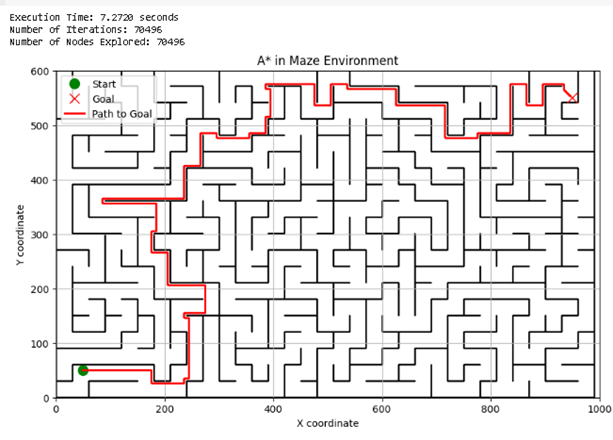
\includegraphics[width=0.7\textwidth]{Images/CH_4/4.1.png}
    \caption{A* path planning in a complex maze environment showing the optimal deterministic path from start to goal.}
    \label{fig:4.1}
\end{figure}


\subsection{RRT* Planning Formulation}

RRT* is a sampling based motion planning algorithm that incrementally builds a search tree within the collision free configuration space. Rather than expanding all neighboring states systematically, RRT* samples random points and connects them to the nearest node in the existing tree.

The cost update for a newly added node is defined as:

\begin{equation}
Cost(x_{new}) = Cost(x_{parent}) + c(x_{parent}, x_{new})
\end{equation}

where $x_{parent}$ denotes the nearest existing node in the search tree selected for extension, and $c(x_{parent}, x_{new})$ represents the incremental cost associated with the edge connecting the parent node to the newly generated node.

Through a rewiring mechanism, RRT* improves solution quality over time by reconnecting nearby nodes if a lower cost path is discovered. While this approach reduces systematic grid expansion, it may generate inefficient exploration in maze environments.

\begin{figure}[h]
    \centering
    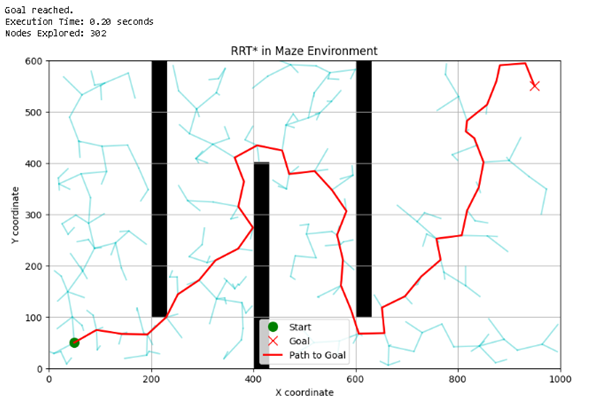
\includegraphics[width=0.7\textwidth]{Images/CH_4/4.2.png}
    \caption{RRT* path planning in a simple maze environment showing the optimal deterministic path from start to goal.}
    \label{fig:4.2}
\end{figure}

Figure \ref{fig:4.2} shows RRT* operating in a structurally simple maze with larger free space regions, where convergence occurs rapidly with limited node expansion and low computational cost. In contrast, Figure \ref{fig:4.3} presents the same algorithm in a more complex maze with dense obstacle distribution and imposed safety margins. The increased structural constraint results in substantially higher node exploration and execution time, reflecting greater search effort before a feasible path is established. This comparison highlights the sensitivity of RRT* performance to environmental complexity.

\begin{figure}[h]
    \centering
    % Figure 4.3 placeholder
    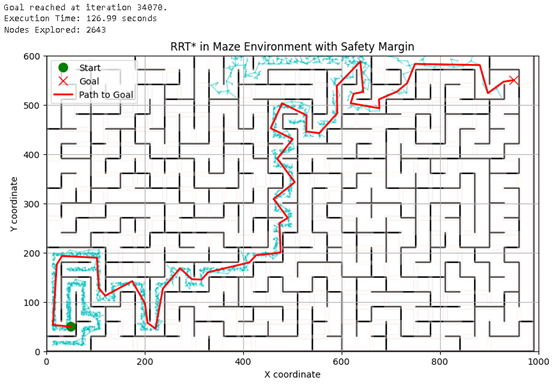
\includegraphics[width=0.7\textwidth]{Images/CH_4/4.3.png}
    \caption{RRT* path planning in a Complex maze environment showing the optimal deterministic path from start to goal.}
    \label{fig:4.3}
\end{figure}

\subsection{Adaptive A* RRT* Hybrid Formulation}

The Adaptive A* RRT* method integrates the goal directed structure of A* with the flexible exploration and refinement capability of RRT*. This integration is achieved through two mechanisms: biased sampling guided by A*, and adaptive weighting controlled by the parameter $\lambda$.

The sampling process is structured according to the following probabilistic rule:

\begin{equation}
x_{sample} = 
\begin{cases}
G & \text{with probability } p_{goal} \\
x \sim P_A & \text{with probability } p_{bias} \\
x \sim X_{free} & \text{otherwise}
\end{cases}
\end{equation}

where $G$ denotes the goal state, $P_A$ represents the guidance region derived from the A* generated path, and $X_{free}$ denotes the collision free configuration space. The parameter $p_{goal}$ defines the probability of directly sampling the goal state, while $p_{bias}$ specifies the probability of sampling from the A* informed guidance region. This probabilistic sampling mechanism balances directed progression toward the goal with guided exploration along promising regions of the search space, while preserving uniform sampling in the remaining free space to maintain exploration capability.

This biased sampling strategy ensures that a portion of the samples are drawn from heuristically meaningful regions. As a result, the planner reduces unnecessary exploration in irrelevant maze areas while preserving probabilistic completeness through continued uniform sampling. Second, the hybrid method introduces adaptive weighting using the parameter $\lambda$ to balance heuristic influence and sampling based optimization. The hybrid objective is defined as:

\begin{equation}
J_{hybrid} = (1 - \lambda) \cdot J_{RRT^*} + \lambda \cdot J_{A^*}
\end{equation}

where $J_{RRT^*}$ denotes the cost component associated with the sampling based tree expansion and rewiring process, and $J_{A^*}$ denotes the heuristic guided evaluation component derived from the A* informed guidance. The parameter $\lambda \in [0,1]$ regulates the relative influence of exploration based optimization and deterministic heuristic guidance within the hybrid plane. When $\lambda$ is small, the algorithm behaves closer to RRT*, favoring faster exploration with lower computational cost but potentially longer paths. When $\lambda$ is large, the planner behaves more strongly guided by A*, encouraging aligned trajectories and shorter paths, but increasing computation due to more constrained refinement.

The combination of biased sampling and adaptive weighting allows the planner to adjust dynamically to maze complexity. In simpler environments, the method behaves efficiently with minimal overhead. In highly constrained mazes, heuristic guidance reduces wasted exploration and improves structural alignment of the path. This formulation directly supports the performance observed in the experimental results presented in Section 4.3, particularly in runtime scaling, node growth trends, and lambda sensitivity analysis.

\section{Simulation Results and Discussion}

This section presents a complete experimental evaluation of the proposed Adaptive A* RRT* algorithm using all results provided in the uploaded figures and tables. The discussion is organized in a way that moves from qualitative path behavior to quantitative scaling trends across maze complexity, and finally to the lambda sensitivity study that explains why the hybrid method behaves differently under different guidance weights. Throughout the analysis, maze difficulty is controlled using the cell size parameter, where a smaller cell size creates narrower corridors, tighter turns, and higher constraint density, which increases the planning burden for all algorithms.

\subsection{Qualitative Path Planning Behavior in Maze Environments}

The qualitative results provide direct insight into how each planner behaves within passage dominated environments. Figure \ref{fig:4.4} presents the path planning comparison at a fixed step size of 10 px and cell size of 200 px. In this configuration, the maze structure is relatively coarse, and the navigable passages are wider; therefore, all three algorithms successfully reach the goal with stable trajectories. The A* path closely follows a geometrically aligned short route through the available passages, which is consistent with its grid based optimal behavior. The RRT* trajectory exhibits noticeable lateral deviation, particularly near the long horizontal passage and during the final approach toward the goal, since random sampling does not inherently maintain alignment within a narrow navigation channel unless sampling density is sufficiently high. The hybrid trajectory appears more structured than RRT*, reducing side deviations and maintaining stronger alignment with the dominant passage direction. This indicates that heuristic guidance from the A* component influences the sampling and connection process. The runtime values shown in the legend further support this observation: at cell size 200 px, the Hybrid method completes in 0.25 s, slightly faster than RRT* at 0.31 s, whereas A* requires 12.99 s. This demonstrates that even in a less constrained maze configuration, systematic grid expansion introduces higher computational overhead compared to sampling based approaches.

\begin{figure}[h]
    \centering
    % Figure 4.4 placeholder
    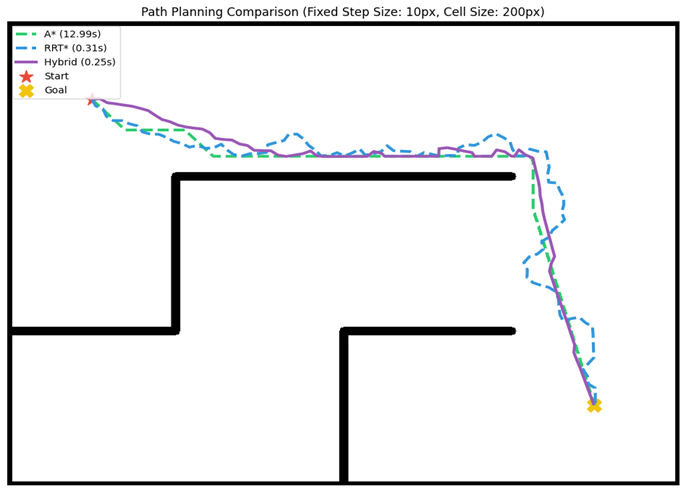
\includegraphics[width=0.7\textwidth]{Images/CH_4/4.4.png}
    \caption{A comparison of A*, RRT*, and Hybrid path planning algorithms in navigating a grid environment, cell size 200px, showing the efficiency, smoothness, and time taken to reach the goal.}
    \label{fig:4.4}
\end{figure}

When the maze becomes more constrained, the differences between the algorithms become more pronounced. Figure \ref{fig:4.5} presents the comparison at a fixed step size of 10 px and cell size of 120 px. In this configuration, the environment introduces narrower transitions and more frequent directional changes, which typically cause A* to expand a substantially larger number of states before committing to the correct sequence of navigable passages. Similarly, RRT* tends to generate samples in regions that do not contribute to progressing through the restricted openings. In the plotted trajectories, RRT* exhibits the most wandering behavior, including a noticeable detour in the lower passage region before stabilizing toward the right side of the maze. A* produces a cleaner path aligned with the navigable structure but requires higher runtime, 36.18 s, reflecting the increased search burden. The hybrid method reaches the goal in 23.07 s, and its trajectory appears more compact than that of RRT* across multiple segments, particularly in the middle transition regions where RRT* expands outward before correcting its direction. This qualitative observation is significant because it explains the quantitative trends presented later: the hybrid method reduces unproductive exploration through heuristic guidance from A* while maintaining flexibility via RRT* connectivity and rewiring when the navigable pathways change direction.

\begin{figure}[h]
    \centering
    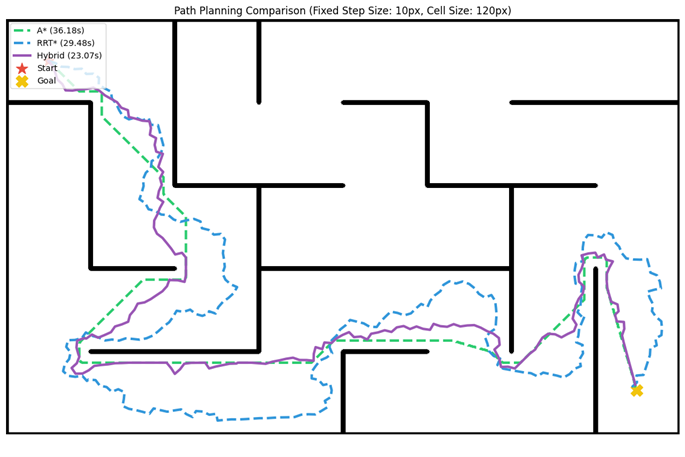
\includegraphics[width=0.7\textwidth]{Images/CH_4/4.5.png}
    % Figure 4.5 placeholder
    \caption{Path planning comparison of A*, RRT*, and Hybrid algorithms in a more complex environment, showing each algorithm’s performance in terms of path smoothness and execution time.}
    \label{fig:4.5}
\end{figure}

The qualitative results therefore establish an important observation: in maze environments, A* typically produces the most geometrically aligned and structurally consistent route, but its computational cost increases significantly as environmental constraints intensify. In contrast, RRT* performs efficiently in relatively open regions but may expend unnecessary effort within structured passage networks. The hybrid approach mitigates excessive exploratory deviations observed in RRT* while avoiding the extensive state expansion characteristic of A* as maze complexity increases.

\subsection{Quantitative Performance Across Maze Complexity}

To evaluate scalability, performance was recorded for four cell sizes, 200, 150, 120, and 100. The full comparative dataset is provided in Table 4.1, while Figures \ref{fig:4.3} to \ref{fig:4.6} provide graphical views of the same performance dimensions. These results collectively show how planning cost increases as corridors tighten and the environment becomes more constrained.

\begin{table}[h]
\centering
\caption{Comparative algorithm performance across maze cell sizes, including time, iterations, nodes, path length, and success outcome.}
\label{tab:4.1}
\begin{tabular}{|c|c|c|c|c|c|c|}
\hline
\textbf{Cell Size} & \textbf{Algorithm} & \textbf{Time (s)} & \textbf{Iterations} & \textbf{Nodes} & \textbf{Path Length} & \textbf{Success} \\
\hline
200 & A* & 13.35 & 524957 & 25085 & 906.5 & True \\
200 & RRT* & 0.38 & 560 & 338 & 1089.0 & True \\
200 & Hybrid & 0.37 & 433 & 314 & 909.2 & True \\
\hline
150 & A* & 1.87 & 58353 & 12289 & 1021.4 & True \\
150 & RRT* & 1.51 & 1356 & 540 & 1320.0 & True \\
150 & Hybrid & 0.69 & 865 & 473 & 1252.1 & True \\
\hline
120 & A* & 55.09 & 1437922 & 175241 & 1712.9 & True \\
120 & RRT* & 36.8 & 8536 & 2669 & 2209.3 & True \\
120 & Hybrid & 24.42 & 6401 & 2920 & 1964.0 & True \\
\hline
100 & A* & 124.64 & 4209810 & 254379 & 1721.2 & True \\
100 & RRT* & 97.58 & 11143 & 3679 & 2239.7 & True \\
100 & Hybrid & 69.74 & 10454 & 4804 & 2100.7 & True \\
\hline
\end{tabular}
\end{table}

The runtime scaling behavior is illustrated in Figure \ref{fig:4.6}. At the most constrained configuration, corresponding to a cell size of 100, the computational burden becomes dominant and the performance separation between the algorithms is most pronounced. A* requires 124.64 s, RRT* requires 97.58 s, and the hybrid method requires 69.74 s. This represents a substantial improvement: the hybrid approach reduces runtime by approximately 44\% relative to A* and 29\% relative to RRT* under the highest structural complexity. The hybrid method remains faster than RRT* because pure RRT* continues to generate exploratory samples near narrow passage boundaries and dead end regions before converging to a stable transition sequence. In contrast, the hybrid planner is guided earlier toward the structurally relevant path suggested by A*, thereby reducing unnecessary expansions.

At a cell size of 120, the same trend persists: A* records 55.09 s, RRT* records 36.80 s, and the hybrid method records 24.42 s. This indicates that even at moderate structural complexity, the hybrid method maintains a consistent computational advantage. At cell size 150, all algorithms exhibit significantly reduced runtime; however, the relative ordering remains unchanged, with A* at 1.87 s, RRT* at 1.51 s, and the hybrid method at 0.69 s. This demonstrates that in less constrained environments, the hybrid approach preserves the efficiency of sampling based expansion while still benefiting from heuristic guidance. At cell size 200, both RRT* and the hybrid method complete extremely quickly, at 0.38 s and 0.37 s respectively, whereas A* remains comparatively higher at 13.35 s. This behavior is characteristic of grid based planning, where even in simplified environments, systematic state evaluation introduces additional computational overhead compared to sampling based methods that can rapidly establish connectivity through wider navigable regions.

\begin{figure}[h]
    \centering
    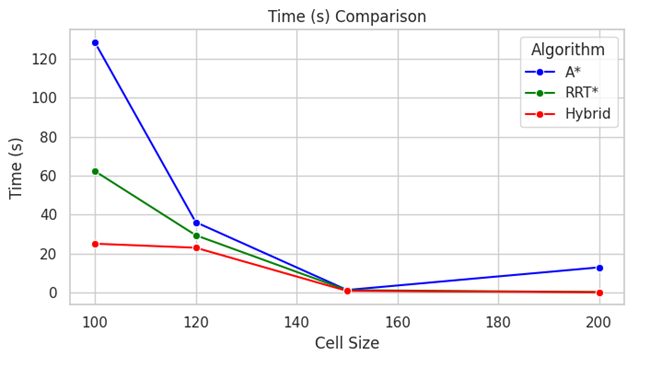
\includegraphics[width=0.7\textwidth]{Images/CH_4/4.6.png}
    % Figure 4.6 placeholder
    \caption{Time comparison of A*, RRT*, and Hybrid algorithms with respect to cell size, highlighting the varying execution times for each algorithm.}
    \label{fig:4.6}
\end{figure}

Iteration counts provide further structural insight into the observed runtime differences. Figure \ref{fig:4.7} illustrates that the number of iterations required by A* increases sharply as the maze becomes more constrained. Table 4.1 confirms the magnitude of this scaling effect at cell size 100, where A* requires 4,209,810 iterations, while RRT* and the Hybrid method remain near ten thousand, at 11,143 and 10,454 iterations respectively. This substantial disparity explains the rapid growth in A* computation time under high structural complexity.

The Hybrid method consistently reduces iteration demand relative to RRT* across most cell sizes. For example, at cell size 150, RRT* requires 1,356 iterations whereas the Hybrid method requires 865. At cell size 200, RRT* requires 560 iterations compared to 433 for the Hybrid approach. These results indicate that heuristic guidance improves the efficiency of sampling based expansion, not only the final path quality.

In structured maze environments, the primary challenge is not simply minimizing geometric distance, but identifying the correct sequence of navigable transitions that leads to the goal. Guided sampling reduces the number of unsuccessful exploratory branches and limits repeated attempts within incorrect passage segments. Consequently, the total number of sampling cycles required for convergence is significantly reduced.

\begin{figure}[h]
    \centering
    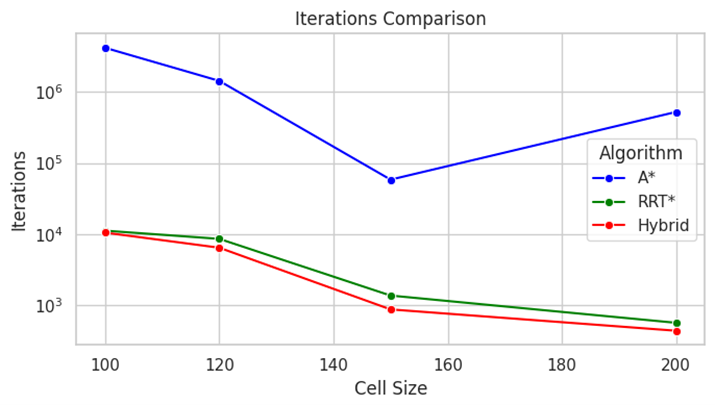
\includegraphics[width=0.7\textwidth]{Images/CH_4/4.7.png}
    % Figure 4.7 placeholder
    \caption{Iterations comparison of A*, RRT*, and Hybrid algorithms with respect to cell size, illustrating the number of iterations required by each algorithm as cell size.}
    \label{fig:4.7}
\end{figure}

Node utilization provides an additional perspective on algorithmic efficiency, as it reflects the extent to which the search space is explored and retained during planning. Figure \ref{fig:4.8} illustrates that A* orders of magnitude more nodes than the other methods, which is consistent with its systematic grid expansion strategy. Table 4.1 shows that at cell size 100, A* expands 254,379 nodes, whereas RRT* expands to 3,679 nodes and the Hybrid method expands 4,804 nodes. Although the Hybrid method uses slightly more nodes than RRT* in the most constrained case, this observation should not be interpreted as a limitation. The Hybrid approach incorporates both sampling based expansion and guided refinement mechanisms, enabling it to maintain additional candidate nodes near critical transition regions while still achieving faster convergence overall.

Importantly, the additional nodes retained by the Hybrid method do not translate into increased runtime; in fact, the total computation time remains significantly lower than that of RRT* at the same complexity level. In less constrained environments, the Hybrid method demonstrates clear improvement over RRT* in node utilization. For example, at cell size 150, the Hybrid method uses 473 nodes compared to 540 for RRT*, and at cell size 200, it uses 314 nodes compared to 338 for RRT*. These results indicate that as structural constraints decrease and navigable regions widen, the Hybrid approach achieves both reduced node usage and lower runtime relative to RRT*.

\begin{figure}[h]
    \centering
    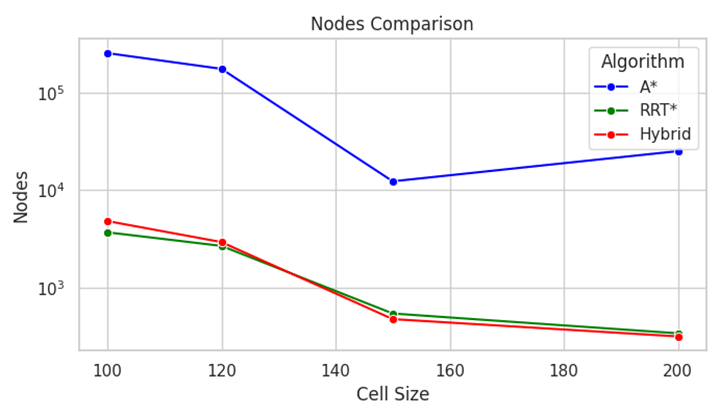
\includegraphics[width=0.7\textwidth]{Images/CH_4/4.8.png}
    % Figure 4.8 placeholder
    \caption{Nodes comparison of A*, RRT*, and Hybrid algorithms against cell size, showing how the number of nodes varies as cell size changes.}
    \label{fig:4.8}
\end{figure}

Path length results, presented in Figure \ref{fig:4.9} and Table 4.1, reflect solution quality across varying maze complexities. As expected, A* produces the shortest paths at all cell sizes due to its grid based optimal search formulation. In contrast, RRT* generates the longest paths, particularly in more structurally constrained environments, reflecting its tendency to exhibit exploratory deviation prior to convergence and its limited structural alignment during early sampling stages. The Hybrid method consistently reduces path length relative to RRT* at every cell size while remaining close to A* in less constrained settings. For instance, at cell size 200, A* achieves a path length of 906.5, while the Hybrid method achieves 909.2, effectively matching grid level optimality while completing in 0.37 s. At cell size 150, A* produces 1021.4, RRT* produces 1320.0, and the Hybrid method produces 1252.1. Although the Hybrid approach does not reach the strict optimality of A*, it demonstrates a clear improvement over RRT*, indicating an effective balance between solution quality and computational efficiency.

At cell size 120, the separation becomes more pronounced: A* yields 1712.9, RRT* yields 2209.3, and the Hybrid method yields 1964.0. The reduction achieved by the Hybrid method relative to RRT* is substantial, as it limits excessive exploratory detours observed in sampling based expansion. However, the Hybrid path remains longer than that of A*, which is consistent with its design objective: prioritizing computational feasibility and stable convergence rather than strict shortest path guarantees. The same trend persists at cell size 100, where A* achieves 1721.2, RRT* achieves 2239.7, and the Hybrid method achieves 2100.7.

\begin{figure}[h]
    \centering
    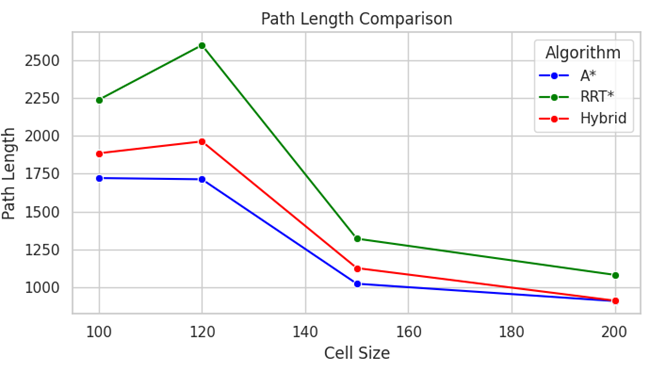
\includegraphics[width=0.7\textwidth]{Images/CH_4/4.9.png} 
    % Figure 4.9 placeholder
    \caption{Path length comparison of A*, RRT*, and Hybrid algorithms with respect to cell size, showing how the path length changes as the cell size increases.}
    \label{fig:4.9}
\end{figure}

Taken together, Figures \ref{fig:4.7} to \ref{fig:4.9} and Table 4.1 support a clear conclusion across maze complexity. A* provides the best path optimality but becomes computationally expensive at high constraint density, RRT* remains feasible but produces longer paths and wastes exploration effort, and the hybrid method consistently improves runtime and convergence behavior while also improving path quality relative to RRT*, especially as the environment becomes more complex. Importantly, Table 4.1 shows that all methods succeed in reaching the goal in all tested cases, therefore the comparison is not about feasibility, it is about efficiency and quality.

\subsection{Lambda Sensitivity Study and Practical Interpretation}

The second part of the results investigates how hybrid behavior changes when the guidance weight lambda is varied. This analysis is essential because it explains why the hybrid method sometimes behaves close to RRT* and sometimes behaves closer to A*. The lambda dataset is presented in Table 4.2, and the trends are visualized in Figures \ref{fig:4.12} to \ref{fig:4.14}. In addition, Figures \ref{fig:4.10} and \ref{fig:4.11} provide qualitative path evidence at the same cell size, showing how the trajectory changes under different lambda settings.

\begin{figure}[h]
    \centering
    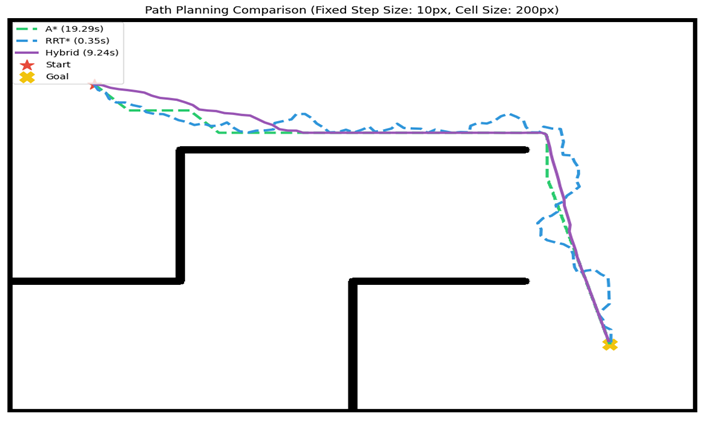
\includegraphics[width=0.7\textwidth]{Images/CH_4/4.10.png}
    % Figure 4.10 placeholder
    \caption{Shows another cell size 200 px run where the hybrid runtime is only 0.41 s, matching the lambda 0.1 case}
    \label{fig:4.10}
\end{figure}

\begin{figure}[h]
    \centering
    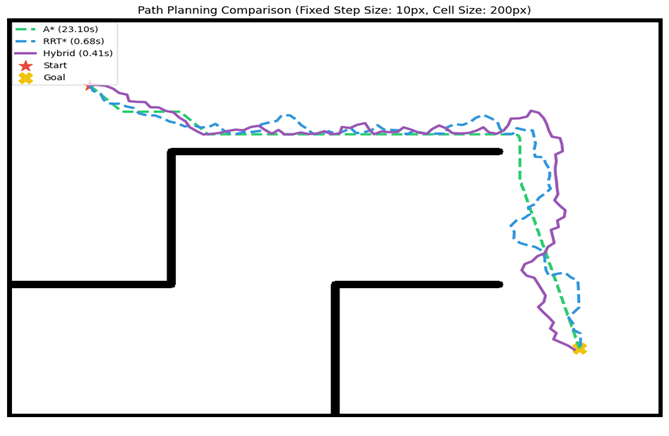
\includegraphics[width=0.7\textwidth]{Images/CH_4/4.11.png}
    % Figure 4.11 placeholder
    \caption{Shows the path planning comparison at cell size 200 px where the hybrid runtime is 9.24 s, matching the lambda 1.0 case}
    \label{fig:4.11}
\end{figure}

\begin{table}[h]
\centering
\caption{Performance metrics for different lambda values, including time, iterations, nodes, and path length.}
\label{tab:4.2}
\begin{tabular}{|c|c|c|c|c|}
\hline
\textbf{Lambda} & \textbf{Time (s)} & \textbf{Iterations} & \textbf{Nodes} & \textbf{Path Length} \\
\hline
0.1 & 0.41 & 650 & 355 & 1100.0 \\
0.2 & 0.29 & 498 & 291 & 1010.0 \\
0.3 & 0.30 & 541 & 334 & 1000.0 \\
0.4 & 0.39 & 593 & 397 & 977.7 \\
0.5 & 0.37 & 600 & 405 & 951.8 \\
0.6 & 0.74 & 601 & 406 & 941.5 \\
1.0 & 9.24 & 2873 & 1796 & 864.7 \\
\hline
\end{tabular}
\end{table}

Figure \ref{fig:4.12} shows time versus lambda. The time curve remains low and stable between lambda 0.1 and 0.5, then begins to rise at 0.6, and finally increases sharply at lambda 1.0. Table 4.2 provides the exact values, at lambda 0.1 time is 0.41 s, at 0.2 it drops to 0.29 s, at 0.3 it is 0.30 s, at 0.4 it is 0.39 s, at 0.5 it is 0.37 s, at 0.6 it increases to 0.74 s, and at 1.0 it jumps to 9.24 s. This pattern indicates that the algorithm has a practical stable zone where guidance improves efficiency without forcing heavy search behavior, and then a high lambda regime where the algorithm becomes much more expensive. In real robotic planning, this is a crucial observation, because it means the best guidance is not necessarily the strongest guidance, there is a point where additional guidance begins to reduce flexibility and increase the internal workload.

\begin{figure}[h]
    \centering
    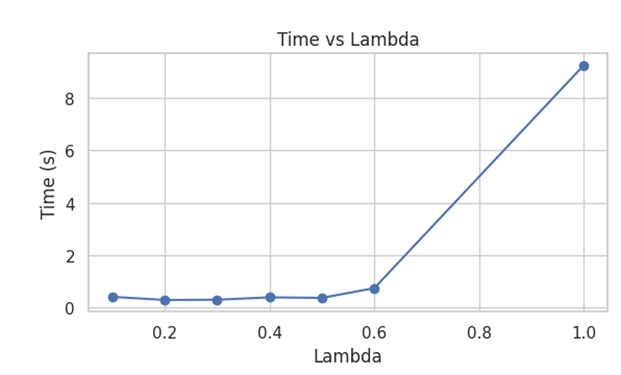
\includegraphics[width=0.7\textwidth]{Images/CH_4/4.12.png}
    % Figure 4.12 placeholder
    \caption{Time versus lambda for Adaptive A* RRT*.}
    \label{fig:4.12}
\end{figure}

The reason for time increases is explained by the node and iteration growth shown in Figure \ref{fig:4.13} and the exact values in Table 4.2. For lambda values from 0.1 to 0.6, the node count stays in a narrow band, from 291 to 406 nodes, and iterations remain near 500 to 650. However, at lambda 1.0, nodes surge to 1,796 and iterations surge to 2,873. This indicates that at very high lambda the method behaves closer to a strongly guided and heavily refined search, where many more candidate nodes are retained and processed, likely because the planner is enforcing strict adherence behavior rather than allowing simpler exploratory shortcuts. This is consistent with maze planning, if guidance becomes too strict, the algorithm may repeatedly attempt similar constrained corridor transitions and spend more work refining them, rather than allowing a broader sampling approach to find a simpler connection.

\begin{figure}[h]
    \centering
    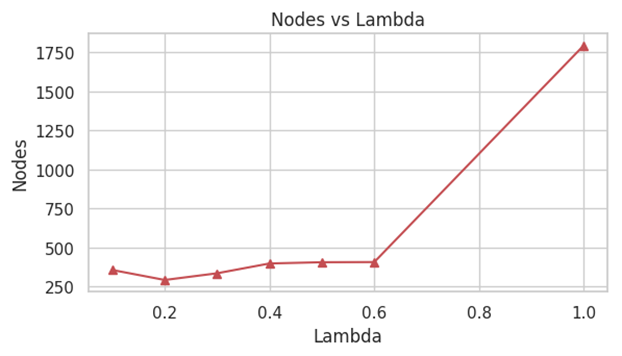
\includegraphics[width=0.7\textwidth]{Images/CH_4/4.13.png}
    % Figure 4.13 placeholder
    \caption{Nodes versus lambda for Adaptive A* RRT*.}
    \label{fig:4.13}
\end{figure}

Path length provides the reward side of this tradeoff, and Figure \ref{fig:4.14} shows that path length steadily decreases as lambda increases. Table 4.2 quantifies this improvement, at lambda 0.1 the path length is 1100.0, at 0.2 it becomes 1010.0, at 0.3 it is 1000.0, at 0.4 it is 977.7, at 0.5 it becomes 951.8, at 0.6 it becomes 941.5, and at 1.0 it reaches 864.7. This means higher lambda improves route optimality, which is expected because stronger guidance encourages the planner to follow more goal directed and corridor efficient routes. However, the critical practical insight is that the improvement is gradual, while the time cost at lambda 1.0 is extreme. Between lambda 0.5 and 1.0, path length improves by about 87.1 units, from 951.8 down to 864.7, but time increases by about 8.87 seconds, from 0.37 to 9.24. For most real time systems, this tradeoff is not attractive, because a small path improvement is being purchased with a large computation penalty.

\begin{figure}[h]
    \centering
    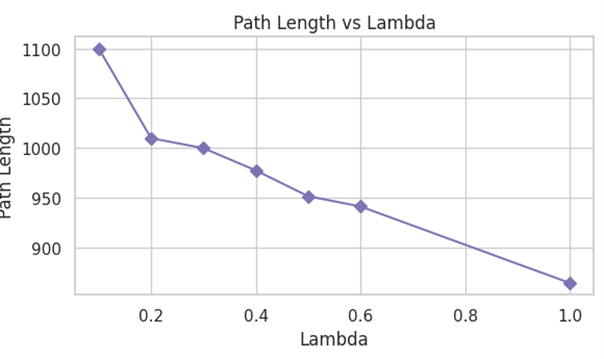
\includegraphics[width=0.7\textwidth]{Images/CH_4/4.14.png}
    % Figure 4.14 placeholder
    \caption{Path length versus lambda for Adaptive A* RRT*.}
    \label{fig:4.14}
\end{figure}

The qualitative trajectory results reinforce this interpretation. Figure \ref{fig:4.11} shows the path planning comparison at cell size 200 px where the hybrid runtime is 9.24 s, matching the lambda 1.0 case. The hybrid path is more tightly aligned with a structured route and shows reduced lateral deviation compared to lower guidance settings, which matches the shorter path length observed numerically. However, this comes with visibly heavier processing cost in runtime. Figure \ref{fig:4.10} shows another cell size 200 px run where the hybrid runtime is only 0.41 s, matching the lambda 0.1 case. In this case, the hybrid path demonstrates more variation near the final descent region, reflecting a less constrained guidance profile. In other words, the qualitative plots show the same concept as the table, lower lambda produces faster solutions with slightly less direct paths, higher lambda produces more direct paths at a much higher computational cost.

From an engineering standpoint, the results support selecting lambda in the moderate range where the algorithm achieves strong time performance while still improving path quality substantially. Based strictly on Table 4.2, lambda 0.2 is a strong candidate because it gives the lowest time, 0.29 s, the lowest node count, 291, and a meaningful path improvement relative to lambda 0.1, reducing path length from 1100.0 to 1010.0. Lambda 0.5 is also attractive because it maintains low time, 0.37 s, while achieving a significantly shorter path, 951.8, but with higher nodes than lambda 0.2. The key point is that pushing lambda to 1.0 produces the shortest path, but at a computation cost that is disproportionate compared to the path improvement gained.

\section{Summary}

This chapter presented a systematic evaluation of the Adaptive A*–RRT* algorithm for robot navigation across maze environments of varying structural complexity. The experimental results demonstrated that while A* ensures grid-optimal paths, its computational cost increases significantly in highly constrained environments, and RRT* reduces grid expansion but introduces exploratory inefficiencies. The proposed hybrid approach effectively balances heuristic guidance and adaptive sampling, achieving reduced computation time and maintaining high success rates while preserving near-optimal path quality. The lambda sensitivity analysis further highlighted the importance of moderate guidance weighting to balance efficiency and optimality. Overall, the findings confirm that Adaptive A*–RRT* provides a robust, scalable, and computationally efficient solution for constrained navigation problems.
\chapter{Development and Performance Evaluation of the LLM Integrated Driving Transition Advisory System}

This chapter presents the detailed design, implementation, and experimental evaluation of the proposed LLM Based Driving Transition Advisory System (DTAS). It validates the effectiveness of integrating large language models within the autonomous vehicle control pipeline through both qualitative and quantitative analyses. Multiple driving scenarios are simulated in CARLA, including red light handling, obstacle detection, turning maneuvers, and varying traffic density conditions. The performance of Llama3 \cite{dubey2024llama} and Mistral \cite{hamzah2024multimodal} is systematically assessed in terms of explanation quality, response time, semantic similarity, and real time feasibility. In addition, traffic density is incorporated into prompt construction and advisory generation to examine its impact on adaptive driving mode recommendations.

\section{Problem Statement}

Although modern autonomous vehicle \cite{liu2020creating} systems demonstrate significant progress in perception, prediction, planning, and control, a critical limitation remains in terms of interpretability and user trust during driving mode transitions. Conventional control algorithms such as Model Predictive Control (MPC) can generate optimal steering, throttle, and braking commands; however, they do not provide human understandable explanations for their decisions. This lack of transparency becomes particularly significant in semi autonomous environments, where responsibility shifts between automated control and the human driver.

During transitions between autonomous and manual modes, drivers often lack clear insight into why certain actions are taken, such as sudden braking, speed reduction, route modification, or obstacle avoidance. The absence of explanatory feedback can reduce driver confidence, create uncertainty, and potentially delay appropriate human intervention in complex traffic scenarios. Moreover, existing autonomous pipelines primarily focus on control accuracy and safety constraints, while limited emphasis is placed on real time advisory communication that aligns system behavior with human understanding.

Another challenge arises in dynamically changing traffic environments. Factors such as obstacle presence, traffic signal states, and local traffic density influence driving decisions, yet these contextual elements are not explicitly translated into interpretable advisory messages. Without a structured mechanism to fuse contextual indicators with control outputs, the system remains technically functional but cognitively opaque to the user.

Therefore, there is a need for a framework that can operate alongside the autonomous control pipeline without interfering with safety critical operations, while simultaneously generating concise, context aware, and human readable explanations. Such a system must function in real time, maintain low latency, and adapt to varying traffic conditions, including density aware scenarios. Addressing this problem forms the foundation of the proposed LLM Integrated Driving Transition Advisory System (DTAS), which aims to bridge the gap between automated vehicle control and human interpretability.

\section{Proposed System Framework}

The proposed Driving Transition Advisory System (DTAS) extends a conventional autonomous vehicle pipeline by introducing an interpretability layer based on large language models. The architecture, illustrated in Figure \ref{fig:3.1}, follows a modular design in which sensing, perception, prediction, localization, planning, control, and LLM based advisory generation operate in a structured and sequential manner. Each component performs a well defined function, and information flows deterministically from sensor acquisition to low level control, while the LLM operates in parallel to provide explanatory feedback without interfering with safety critical execution.

\subsection{Sensor Layer}

The sensor layer forms the foundation of autonomous vehicle architecture \cite{yeong2021sensor}. In the CARLA simulation environment, multiple sensing modalities are employed to capture environmental and vehicle state information.

The teleport camera provides a stabilized ego centric view of the vehicle's surroundings, enabling object visualization and scene interpretation. The wide angle camera captures a broader field of view, which is essential for detecting lane boundaries, traffic signs, and traffic light states. LiDAR provides three dimensional point cloud data, allowing accurate spatial localization of nearby obstacles and vehicles. Unlike camera only systems, LiDAR contributes reliable distance measurements that enhance robustness under complex spatial arrangements. The GPS module supplies global positioning information used for localization within the simulated map.

These sensors collectively generate raw data streams that are continuously updated at each simulation tick. This raw data is forwarded to the perception layer for semantic interpretation. As shown in Figure \ref{fig:5.1}.

\begin{figure}[h]
    \centering
    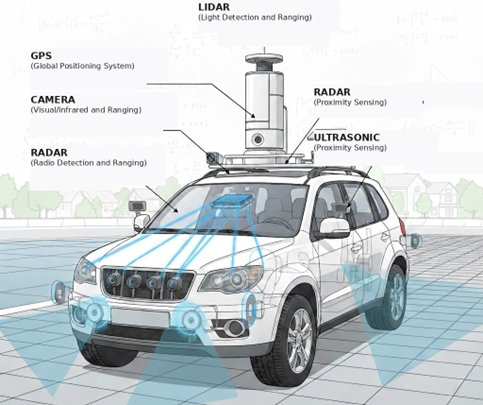
\includegraphics[width=0.8\textwidth]{Images/CH_5/Figure 5.1.png}
    % Figure 5.1 placeholder
    \caption{An autonomous vehicle equipped with multiple sensing technologies LiDAR, GPS, Camera, Radar, and Ultrasonic sensors working together to enable self driving capabilities through real time detection, positioning, and environmental awareness.Image generated using Google Gemini.}
    \label{fig:5.1}
\end{figure}

\subsection{Perception Module}

The perception module converts raw sensor inputs into structured environmental representations. This stage includes multiple subcomponents responsible for extracting meaningful information from visual and spatial data. As shown in Figure \ref{fig:5.2}. Object detection identifies surrounding vehicles, pedestrians, and static obstacles using camera and LiDAR inputs. Detected objects are represented through bounding boxes and positional coordinates. Object tracking maintains temporal consistency by associating detections across consecutive frames, enabling estimation of velocity and motion continuity.

\begin{figure}[h]
    \centering
    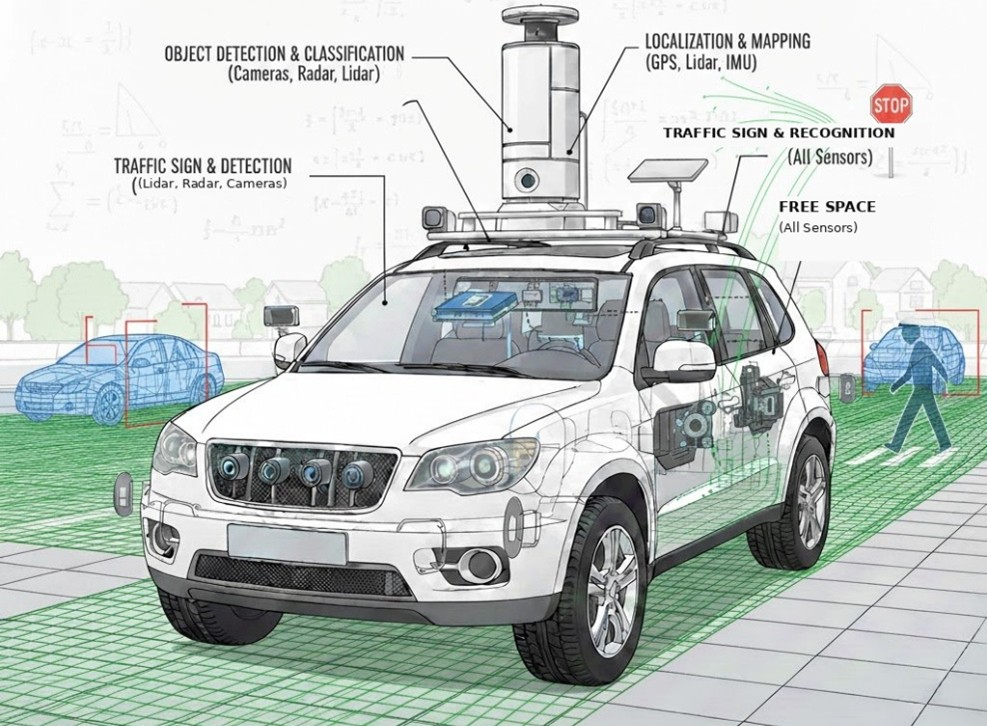
\includegraphics[width=0.8\textwidth]{Images/CH_5/Figure 5.2.jpg}
    % Figure 5.2 placeholder
    \caption{An autonomous vehicle using Cameras, Radar, LiDAR, GPS, and IMU sensors for real time object detection, mapping, traffic sign recognition, and free space estimation.Image generated using Google Gemini.}
    \label{fig:5.2}
\end{figure}

Lane detection extracts lane boundary information from camera images, ensuring that the ego vehicle maintains lane discipline. Traffic sign detection recognizes regulatory and warning signs, such as speed limits or stop signs, which influence driving behavior. Traffic light detection determines the state of signals (red, yellow, green), which is encoded as a structured flag for decision making.

The output of the perception module is a structured scene description containing detected objects, signal states, and lane information. This structured representation forms the basis for predictive and planning decisions.

\subsection{Prediction and Localization}

The prediction module estimates the potential future motion of dynamic agents in the environment. Based on current velocity and trajectory information, it forecasts short term movement patterns of surrounding vehicles. This predictive capability is essential for proactive maneuver planning, particularly in obstacle avoidance and intersection scenarios. As shown in Figure \ref{fig:5.3}.

Simultaneously, localization determines the precise position and orientation of the ego vehicle within the digital map. Using GPS and mapping information, the system maintains spatial alignment with the CARLA Town04 environment. Mapping provides detailed road topology, including lane geometry, intersections, and traffic signal placements. Accurate localization ensures that trajectory planning aligns with actual road structure.

\begin{figure}[h]
    \centering
    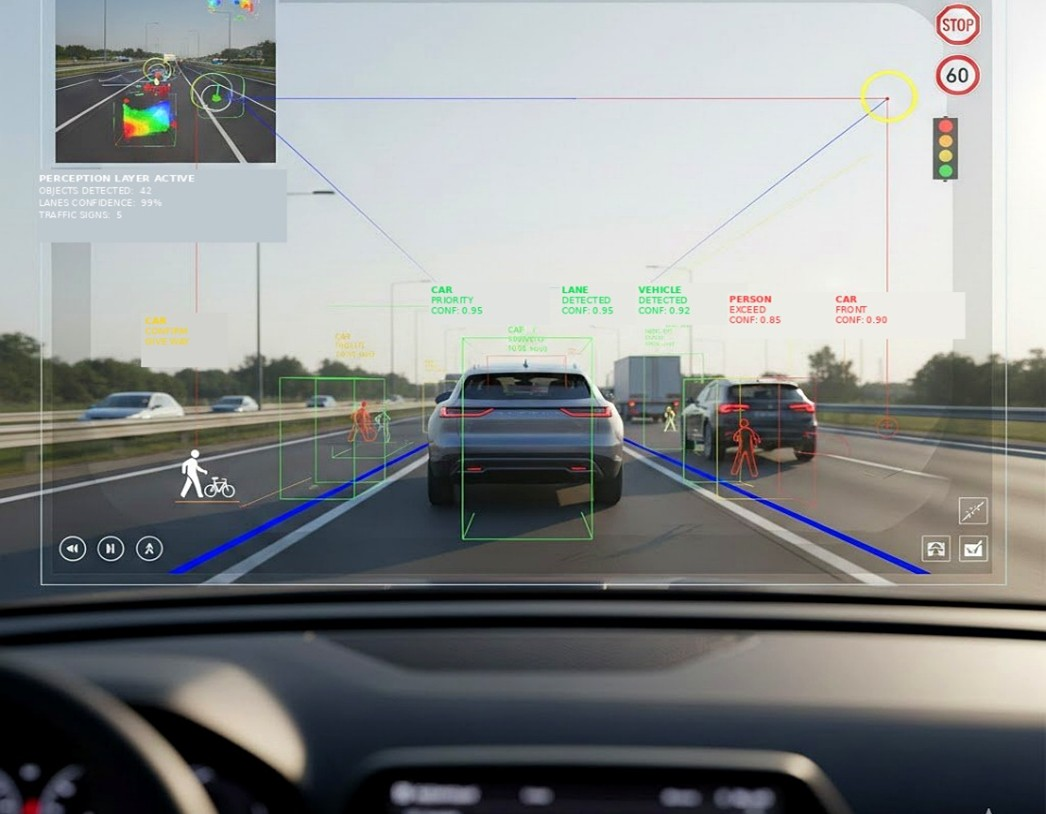
\includegraphics[width=0.7\textwidth]{Images/CH_5/Figure 5.3.jpg}
    % Figure 5.3 placeholder
    \caption{Perception layer showing real time detection of lanes, vehicles, pedestrians, and traffic signs.Image generated using Google Gemini.}
    \label{fig:5.3}
\end{figure}

\subsection{Planning Layer}

The planning stage operates hierarchically and consists of route planning, behavior planning \cite{wang2023drivemlm}, and trajectory planning \cite{geisslinger2023ethical}. Route planning \cite{sheng2021trust} determines the global path between the starting point and the destination using map based navigation. Behavior planning evaluates contextual conditions such as obstacle presence, traffic light states, and traffic rules to decide high level maneuvers. For example, when a red light is detected, the behavior planner selects a stopping maneuver; when an obstacle is present ahead, it selects a deceleration or avoidance strategy. As shown in Figure \ref{fig:5.4}.

\begin{figure}[h]
    \centering
    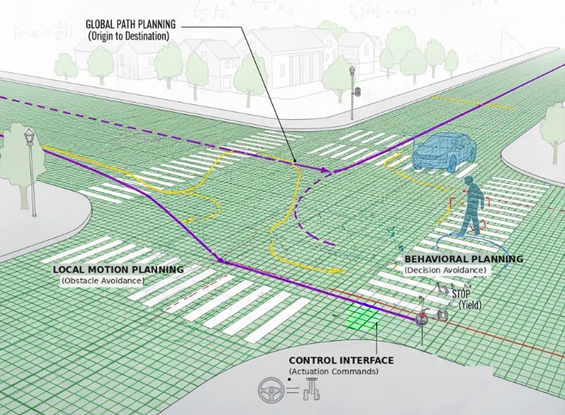
\includegraphics[width=0.7\textwidth]{Images/CH_5/Figure 5.4.png}
    % Figure 5.4 placeholder
    \caption{End-to-end autonomous driving planning architecture combining global routing, behavioral planning, and local motion control.Image generated using Google Gemini.}
    \label{fig:5.4}
\end{figure}

Trajectory planning \cite{lee2017trajectory} converts high level decisions into a smooth and dynamically feasible path that satisfies vehicle kinematic constraints. It generates a sequence of waypoints and target velocities that guide the vehicle safely along the intended path. The output of the planning module is encapsulated in a structured message containing waypoint coordinates, speed targets, traffic signal states, obstacle indicators, and local traffic density values. Traffic density \cite{munoz2003traffic} is computed by counting the number of nearby agents within a predefined radius around the ego vehicle. This density metric is later incorporated into advisory reasoning.

\subsection{Control Module}

The Model Predictive Control (MPC) \cite{kouvaritakis2016model} module is responsible for tracking the planned trajectory and generating optimal low level control commands at each simulation step. MPC operates over a finite prediction horizon, where it minimizes the deviation between the reference trajectory and the predicted vehicle motion. The optimization process considers vehicle kinematic constraints, steering limits, acceleration bounds, and braking capabilities. By continuously updating control inputs, the controller ensures smooth trajectory tracking and stability under dynamic traffic conditions. The outputs include steering angle, throttle input, and brake pressure, which are applied directly to the ego vehicle within the CARLA simulation environment.

\begin{figure}[h]
    \centering
    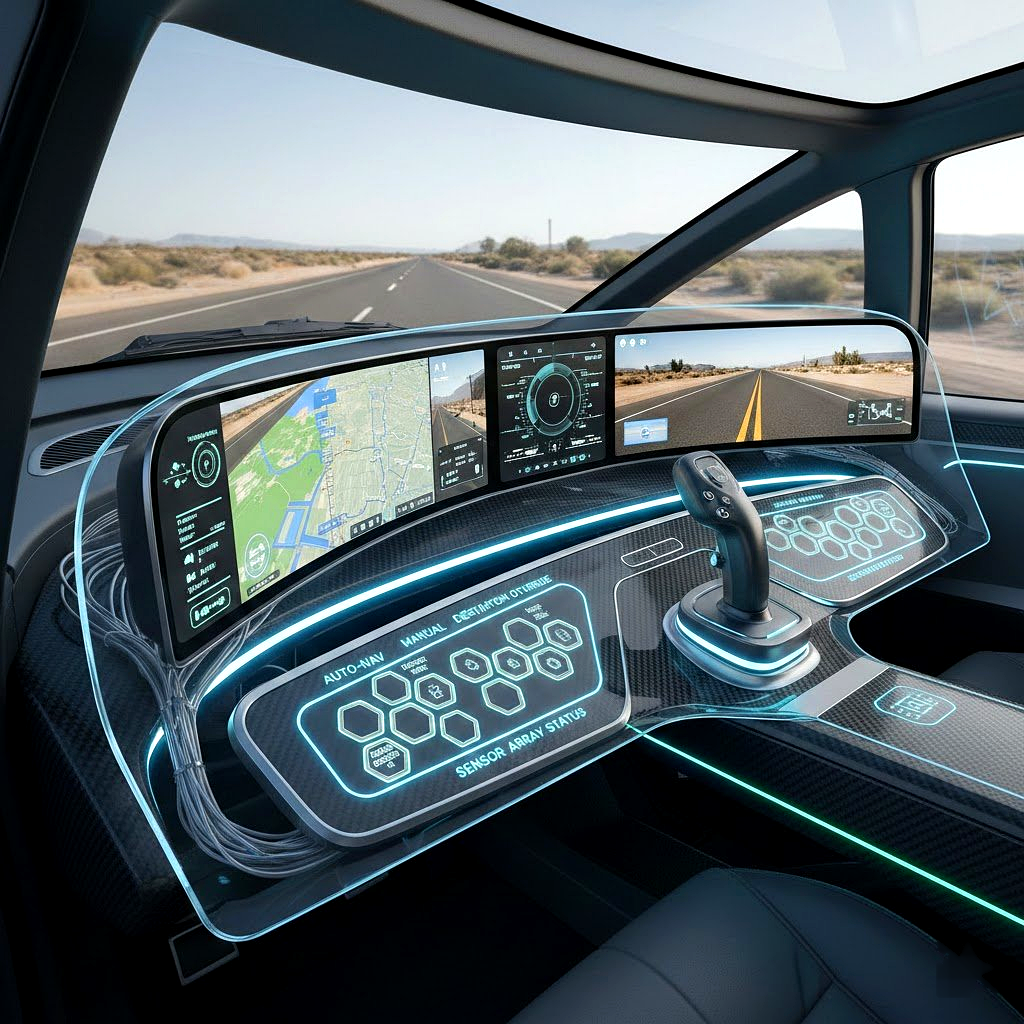
\includegraphics[width=0.6\textwidth]{Images/CH_5/Figure 5.5.png}
    % Figure 5.5 placeholder
    \caption{Visualization of the autonomous vehicle control layer showing steering input, velocity regulation, and real time actuation feedback within the integrated control architecture.Image generated using Google Gemini.}
    \label{fig:5.5}
\end{figure}

The control module is deterministic and safety critical in nature. It guarantees that trajectory execution remains stable regardless of environmental complexity or advisory reasoning outputs. Even under varying traffic density, obstacle presence, or signal changes, the MPC \cite{rokonuzzaman2021model} maintains adherence to safety margins and dynamic feasibility constraints. As shown in Figure \ref{fig:5.5}. Importantly, the LLM advisory layer does not modify or override any control commands. This architectural separation ensures that interpretability enhancements do not compromise system reliability or operational safety.

\subsection{LLM Based Advisory Layer}

The LLM based advisory layer operates in parallel with the control module and functions as an interpretability extension to the autonomous driving pipeline. At each simulation tick, structured vehicle state parameters including steering angle, throttle percentage, brake pressure, velocity, traffic light state, obstacle presence, traffic sign detection, and local traffic density are extracted and formatted into a prompt. This structured representation captures both control actions and environmental context, allowing the language model to reason about the vehicle's operational state.

Traffic density is calculated by counting nearby vehicles and obstacles within a predefined spatial radius around the ego vehicle. This parameter reflects the level of environmental complexity and influences advisory tone and recommendation strength. In low density conditions, the LLM typically confirms safe continuation of autonomous mode. In higher density environments, explanations may emphasize increased maneuvering difficulty and suggest heightened driver awareness or potential mode transition. The advisory output remains purely communicative and does not interfere with trajectory execution or control stability.

To demonstrate the operational synchronization between deterministic control execution and language based reasoning, real time runtime snapshots of the integrated CARLA LLM framework are presented in Figures \ref{fig:5.6}. The terminal interface displays structured state variables extracted at each simulation tick, including vehicle position, longitudinal velocity, steering angle, throttle input, brake pressure, traffic light state, obstacle detection status, and local traffic density.

\begin{figure}[h]
    \centering
    \includegraphics[width=0.7\textwidth]{Images/CH_5/Figure 5.6.png}
    % Figure 5.6 placeholder
    \caption{Real time synchronization between structured vehicle state extraction and LLM advisory generation, showing terminal based prompt construction alongside the corresponding CARLA driving scenario.}
    \label{fig:5.6}
\end{figure}

\subsection{Architectural Integration and Data Flow}

The DTAS architecture follows a structured data flow beginning with sensor acquisition, followed by perception, prediction, localization, planning, and control execution. Each module processes structured information and forwards it sequentially to the next stage. In parallel to the control module, selected state and contextual parameters are transmitted to the LLM advisory layer. This dual path architecture preserves the integrity of the primary control loop while enabling real time explanatory reasoning. 

By isolating deterministic control from probabilistic language based reasoning, the framework maintains operational stability while enhancing transparency. The integration strategy ensures that advisory communication remains synchronized with real time vehicle behavior without introducing additional latency into the control loop. This design enables the system to achieve both technical reliability and human level interpretability during driving mode transitions, particularly under varying traffic density conditions.

\section{Experimental Setup}

The experimental evaluation of the proposed Driving Transition Advisory System (DTAS) was conducted within the CARLA 0.9.13 autonomous driving simulator. The Town04 environment was selected due to its structured road topology, signalized intersections, and moderate traffic complexity, which provide realistic urban driving conditions. As shown in Figure \ref{fig:5.7}. The simulation environment enabled controlled evaluation of traffic light interactions, obstacle detection scenarios, turning maneuvers, and varying traffic density conditions. All experiments were executed using Python 3.9.12 on an Ubuntu 18.04.6 LTS workstation equipped with an 11th Gen Intel\textsuperscript{\textregistered} Core\texttrademark{} i7-11700K CPU, 23.4 GB RAM, and an NVIDIA RTX 3060 GPU. This configuration ensured stable real time simulation and local LLM inference without cloud based dependencies.

\begin{figure}[h]
    \centering
    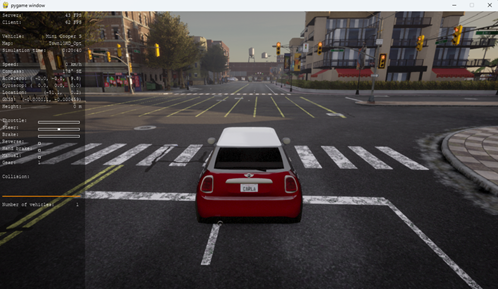
\includegraphics[width=0.7\textwidth]{Images/CH_5/Figure 5.7.png}
    % Figure 5.7 placeholder
    \caption{CARLA simulator scene showing an autonomous vehicle positioned at a signalized urban intersection.}
    \label{fig:5.7}
\end{figure}

The system pipeline integrated the PlanningOperator and MPCOperator modules to generate trajectory and control outputs at each simulation tick. The WaypointsMessage transmitted from planning to control contained waypoint coordinates, target speeds, traffic light states, obstacle flags, and traffic density values. At every control step, vehicle state parameters including position, velocity, steering angle, throttle input, and brake pressure were logged and simultaneously formatted into structured prompts for LLM processing. Both Llama3 and Mistral models were hosted locally to measure inference latency under real time conditions. All generated prompts, LLM responses, and generation times were recorded to enable reproducible evaluation and comparative analysis.

Multiple scenario categories were designed to evaluate system performance under diverse driving conditions. These included: (1) red light stopping scenarios, (2) red light combined with obstacle presence, (3) left turn maneuvers at intersections, (4) obstacle ahead deceleration cases, and (5) open road driving without obstacles. In addition to scenario based evaluation, traffic density variation was introduced by controlling the number of surrounding agents within a predefined radius around the ego vehicle. This allowed assessment of advisory adaptation under low density and high density conditions.

To evaluate the effectiveness of the advisory system, both qualitative and quantitative metrics were employed. Qualitative evaluation focused on the semantic correctness and contextual relevance of generated explanations. Quantitative evaluation included average word count, response time in seconds, and BERTScore for semantic similarity between generated outputs and expected explanations. These metrics provided insight into explanation conciseness, latency performance, and semantic alignment with intended driving behavior. Together, the experimental setup ensured systematic validation of DTAS under controlled yet realistic autonomous driving scenarios.

\section{Results and Discussion}

This section presents the evaluation of the proposed Driving Transition Advisory System (DTAS). The performance of Llama3 and Mistral is analyzed across multiple simulated driving scenarios in CARLA. Qualitative assessment examines the alignment between generated explanations and scene context. Quantitative metrics, including word count, response time, and BERTScore, are evaluated. Together, these results demonstrate the framework's interpretability and real time feasibility.

\subsection{Scenario Based Explanation Generation}

The first evaluation phase focuses on the quality and contextual accuracy of LLM generated explanations across representative driving scenarios. Table 5.1 presents a comprehensive comparison of scenario specific prompts, expected driving behavior, and the corresponding natural language explanations generated by Llama3 and Mistral. Five distinct scenarios were evaluated: red light stopping, red light combined with obstacle presence, left turn maneuvers, obstacle ahead deceleration, and open road driving without obstacles. For each scenario, a structured prompt was constructed incorporating vehicle state parameters including position coordinates, velocity, steering angle, throttle input, brake pressure, traffic light state, and obstacle detection flags. The expected output represents the ideal human understandable description of the vehicle's behavior in that context. Both Llama3 and Mistral successfully captured the essential driving actions, although with notable differences in explanation style and verbosity.
\begin{table*}[ht]
\small
\caption{Scenario wise output: Expected driving behavior, and natural language explanations from Llama3 and Mistral.}
\renewcommand{\arraystretch}{1.2}
\centering
\resizebox{\textwidth}{!}{ % Resize the table to fit within text width
\begin{tabular}{|l|p{4cm}|p{4.5cm}|p{4.5cm}|}
\hline
\textbf{Scenario} & \textbf{Expected Output} & \textbf{Llama3 Explanation} & \textbf{Mistral Explanation} \\
\hline
Red Light & The vehicle is stopping for the red traffic light ahead. & The vehicle is stopped at a red traffic light with caution. & The vehicle has stopped (0 m/s) at (338.82, 22.72), awaiting green signal due to red traffic light ahead. \\
\hline
Red Light + Obstacle & The vehicle is slowing down due to a red traffic light and an obstacle ahead. & The vehicle is slowing down due to an obstacle detection and red traffic light ahead. & The stationary vehicle is at a standstill with no movement, awaiting the green light while detecting an obstacle ahead. \\
\hline
Left Turn & The vehicle is turning left at the next intersection. & The vehicle is slowly moving forward with a gentle left turn at low speed. & The vehicle is accelerating slightly at (160.03, 58.26) with a gentle left turn. No traffic lights ahead. \\
\hline
Obstacle ahead & The vehicle is slowing down to avoid the obstacle ahead. & The vehicle is moving steadily forward while detecting an obstacle ahead. & The vehicle, moving at 3.15 m/s, approaches an open road with an obstacle detected ahead. It maintains speed and continues forward. \\
\hline
No Obstacle Ahead & The vehicle is driving smoothly with no obstacles on the road. & The vehicle is moving forward at a steady pace. & The vehicle is accelerating at a steady pace with a slight turn, heading forward without any stops due to an open road and no traffic lights ahead. \\
\hline
\end{tabular}
}
\end{table*}

\subsection{Visual Analysis of Driving Scenarios}

To provide a comprehensive understanding of the system's behavior in real-world simulated conditions, three representative scenarios from Table 5.1 are analyzed visually: no obstacle ahead, obstacle ahead, and left-turn maneuvers. These scenarios illustrate the capability of both Llama3 and Mistral to generate contextually appropriate explanations based on the structured vehicle state information. Figure \ref{fig:5.8} presents the no-obstacle scenario, where the ego vehicle moves smoothly on an open road without any detected hazards ahead. In this situation, Llama3 provides a concise explanation indicating steady forward movement, while Mistral elaborates with additional contextual details including the absence of traffic lights and confirmation of steady acceleration. Both explanations are semantically accurate and align with the vehicle's observed behavior, although Mistral's output includes more descriptive elements that may enhance user understanding in certain contexts.

\begin{figure}[h]
    \centering
    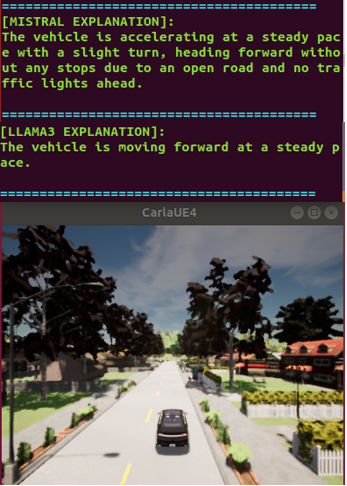
\includegraphics[width=0.5\textwidth]{Images/CH_5/Figure 5.8.png}
    % Figure 5.8 placeholder
    \caption{No obstacle ahead scenario showing the ego vehicle moving smoothly on an open road.}
    \label{fig:5.8}
\end{figure}

Figure \ref{fig:5.9} illustrates the obstacle-ahead scenario, where the perception module detects a potential hazard in the vehicle's forward trajectory. Under these conditions, the control system reduces throttle input and increases brake pressure to maintain safe following distance. Llama3 generates an explanation stating that the vehicle is moving steadily while detecting an obstacle, providing clear acknowledgment of the environmental condition. Mistral's explanation includes additional quantitative details such as the current vehicle speed in meters per second and explicitly confirms that the vehicle maintains its speed while continuing forward. Both models successfully integrate the obstacle detection flag into their explanatory outputs, demonstrating contextual awareness. However, Mistral's inclusion of numerical velocity data may provide drivers with more precise situational awareness, particularly in semi-autonomous environments where the driver must remain vigilant about vehicle dynamics.

\begin{figure}[h]
    \centering
    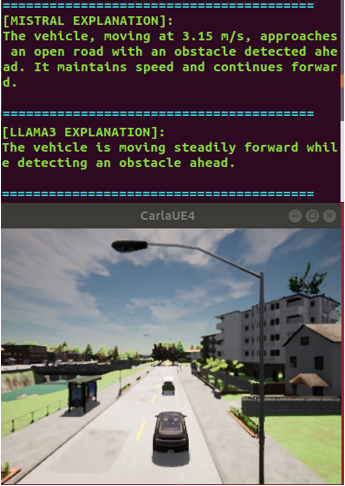
\includegraphics[width=0.5\textwidth]{Images/CH_5/Figure 5.9.png}
    % Figure 5.9 placeholder
    \caption{Obstacle ahead scenario where the perception system detects a forward hazard.}
    \label{fig:5.9}
\end{figure}

The left-turn scenario, presented in Figure \ref{fig:5.10}, evaluates the system's ability to explain lateral maneuvering behavior during intersection navigation. In this case, the steering angle parameter indicates a negative value corresponding to leftward vehicle orientation, while throttle input remains active to maintain forward momentum through the turn. Llama3 provides a straightforward description indicating slow forward movement with a gentle left turn, capturing the essential elements of the maneuver in simple language. Mistral's explanation adds spatial context by referencing the vehicle's position coordinates and explicitly noting the absence of traffic lights ahead, which may influence driver expectations about intersection control requirements. Both models correctly interpret the steering angle sign and direction, demonstrating their capacity to reason about vehicle kinematics. The comparison reveals that while Llama3 prioritizes brevity and directness, Mistral tends toward richer contextual descriptions that may benefit users requiring detailed situational awareness.

\begin{figure}[h]
    \centering
    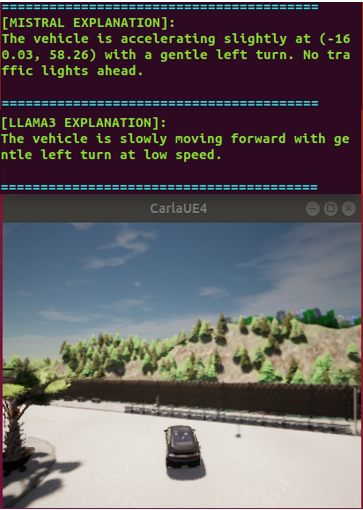
\includegraphics[width=0.5\textwidth]{Images/CH_5/Figure 5.10.PNG}
    % Figure 5.10 placeholder
    \caption{Left-turn scenario demonstrating vehicle lateral maneuvering at an intersection.}
    \label{fig:5.10}
\end{figure}

\subsection{Traffic Density Integration and Advisory Generation}

Beyond basic scenario explanation, the system integrates local traffic density as a contextual parameter influencing advisory message generation. Traffic density is computed by counting the number of surrounding vehicles and obstacles within a predefined spatial radius around the ego vehicle at each simulation tick. This density metric, combined with obstacle presence and traffic signal state information, enables the LLM to generate adaptive driving mode recommendations that reflect environmental complexity. Figure \ref{fig:5.11} demonstrates the low-density advisory scenario, where the surrounding traffic environment contains minimal vehicle interactions and clear road conditions. Under these circumstances, the LLM generates a reassuring message confirming that the road is open and safe, explicitly advising that the vehicle can remain in autonomous mode. This type of advisory supports driver confidence in system capability when environmental conditions are favorable for automated control. The message is concise and actionable, providing clear guidance without overwhelming the driver with unnecessary detail.

\begin{figure}[h]
    \centering
    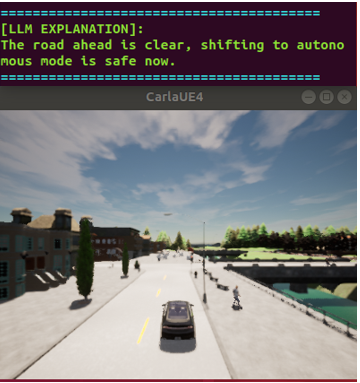
\includegraphics[width=0.6\textwidth]{Images/CH_5/Figure 5.11.png}
    % Figure 5.11 placeholder
    \caption{LLM-generated advisory message for low-density scenario recommending continued autonomous mode.}
    \label{fig:5.11}
\end{figure}

\subsection{Comparative Analysis: Word Count}

Quantitative evaluation of explanation characteristics begins with average word count analysis, presented in Figure \ref{fig:5.12}. This metric reflects the conciseness and verbosity of generated explanations across all evaluated scenarios. Llama3 produces explanations with an average word count of 11.8 words, closely adhering to the prompt instruction requesting responses in 10 to 12 words. This demonstrates Llama3 strong adherence to length constraints and its ability to generate compact, focused explanations without sacrificing semantic correctness. In contrast, Mistral generates significantly longer outputs, averaging 20.7 words per explanation. While this increased verbosity provides additional contextual detail and descriptive elements, it exceeds the specified word limit by approximately 75 percent. The difference suggests distinct model behaviors: Llama3 prioritizes brevity and instruction compliance, whereas Mistral emphasizes comprehensive description even when explicitly constrained. Both approaches have merit depending on application requirements; concise explanations minimize cognitive load and display space requirements, while detailed explanations may enhance understanding in complex scenarios.


\begin{figure}[h]
    \centering
    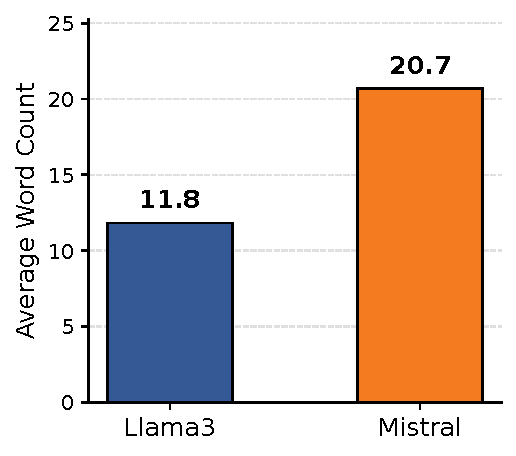
\includegraphics[width=0.6\textwidth]{Images/CH_5/Figure 5.12.pdf}
    % Figure 5.12 placeholder
    \caption{Comparison of average word count between Llama3 and Mistral explanations.}
    \label{fig:5.12}
\end{figure}

\subsection{Comparative Analysis: Generation Time}

Response time performance is critical for real time advisory systems, as excessive latency can reduce the relevance of generated explanations during rapidly changing driving conditions. Figure \ref{fig:5.13} compares the average generation time for Llama3 and Mistral across all evaluated scenarios. Llama3 achieves an average inference time of 0.37 seconds per explanation, demonstrating efficient processing suitable for real time application. This low latency ensures that explanations can be generated and displayed to the driver with minimal delay relative to the actual vehicle state being described. Mistral exhibits an average generation time of 0.60 seconds, representing a 62 percent increase in inference duration compared to Llama3. While still within acceptable bounds for near real time interaction, this additional latency may accumulate over extended driving sessions or during high frequency updates. The correlation between word count and generation time is evident; Llama3 concise outputs are produced more quickly, while Mistral's longer explanations require additional processing. From a practical deployment perspective, Llama3 faster response supports more frequent advisory updates without introducing perceptible lag in the user interface.

\begin{figure}[h]
    \centering
    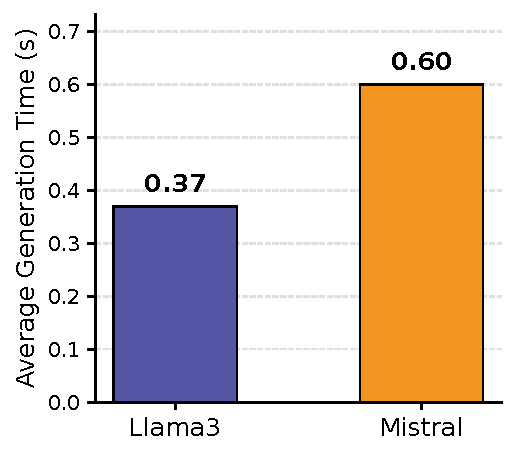
\includegraphics[width=0.6\textwidth]{Images/CH_5/Figure 5.13.pdf}
    % Figure 5.13 placeholder
    \caption{Comparison of average generation time between Llama3 and Mistral models.}
    \label{fig:5.13}
\end{figure}

\subsection{Semantic Similarity Evaluation: BERTScore Analysis}

Beyond surface level metrics such as word count and generation time, the semantic quality of explanations must be assessed to ensure that generated output accurately reflects the intended meaning and contextual correctness. BERTScore provides a robust measure of semantic similarity between generated explanations and expected reference outputs by comparing contextual embeddings derived from pre trained language models. Figure \ref{fig:5.14} presents a scenario wise BERTScore comparison for Llama3 and Mistral across the five evaluated driving conditions. Both models achieve high semantic similarity scores across all scenarios, with BERTScore values consistently above 0.89, indicating strong alignment with expected explanations. For the red light scenario, Llama3 achieves a BERTScore of 0.95, demonstrating near perfect semantic correspondence with the reference output. Mistral achieves 0.90 for the same scenario, still representing high similarity. In the red light plus obstacle scenario, Llama3 attains an exceptional BERTScore of 0.98, while Mistral scores 0.91, both confirming accurate integration of multiple contextual factors into the explanation.

\begin{figure}[h]
    \centering
    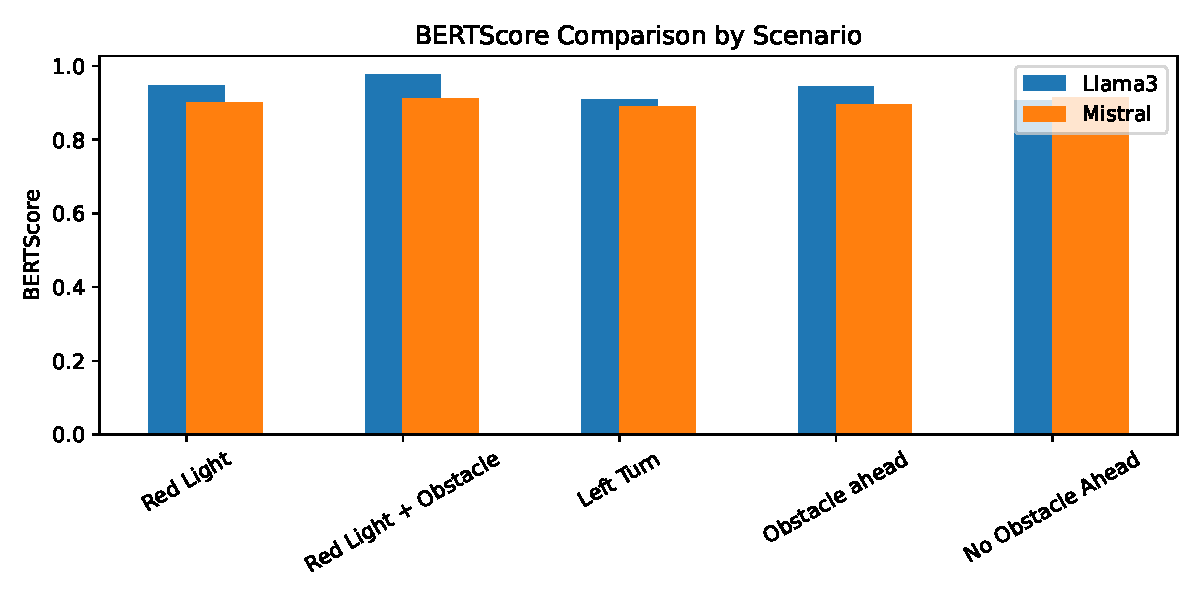
\includegraphics[width=0.7\textwidth]{Images/CH_5/Figure 5.14.pdf}    
    % Figure 5.14 placeholder
    \caption{BERTScore comparison across different driving scenarios for Llama3 and Mistral.}
    \label{fig:5.14}
\end{figure}

\subsection{Detailed Scenario Wise Performance Metrics}

Table 5.2 provides a comprehensive summary of performance metrics for both Llama3 and Mistral across all evaluated scenarios, integrating word count, response time, and BERTScore \cite{zhang2018path} into a unified comparative framework. This detailed breakdown enables scenario specific analysis and reveals performance patterns that may not be apparent from aggregated statistics alone. In the red light scenario, Llama3 generates an 11 word explanation in 0.33 seconds with a BERTScore of 0.95, while Mistral produces an 18 word explanation in 0.57 seconds with a BERTScore of 0.90. Both outputs are semantically strong, although Llama3 demonstrates superior speed and marginally higher semantic alignment. The red light plus obstacle scenario shows similar trends, with Llama3 achieving 0.98 BERTScore in 0.36 seconds (15 words) compared to Mistral's 0.91 BERTScore in 0.46 seconds (19 words). Notably, Llama3 response time remains consistent despite varying scenario complexity, suggesting efficient and stable inference.

\begin{table}[h]
\centering
\caption{Detailed scenario wise comparison of Llama3 and Mistral explanations, showing word count, response time, and BERTScore.}
\label{tab:5.2}
\resizebox{\textwidth}{!}{ % Resize the table to fit within text width
\begin{tabular}{|l|c|c|c|c|c|c|}
\hline
\textbf{Scenario} & \textbf{Llama3} & \textbf{Llama3} & \textbf{Llama3} & \textbf{Mistral} & \textbf{Mistral} & \textbf{Mistral} \\
 & \textbf{Word Count} & \textbf{Time (s)} & \textbf{BERTScore} & \textbf{Word Count} & \textbf{Time (s)} & \textbf{BERTScore} \\
\hline
Red Light & 11 & 0.33 & 0.95 & 18 & 0.57 & 0.90 \\
\hline
Red Light + Obstacle & 15 & 0.36 & 0.98 & 19 & 0.46 & 0.91 \\
\hline
Left Turn & 13 & 0.34 & 0.91 & 17 & 0.59 & 0.89 \\
\hline
Obstacle Ahead & 11 & 0.35 & 0.94 & 21 & 0.65 & 0.90 \\
\hline
No Obstacle Ahead & 9 & 0.30 & 0.91 & 27 & 0.79 & 0.91 \\
\hline
\end{tabular}
}
\end{table}

For the left turn scenario, Llama3 achieves a BERTScore of 0.91 in 0.34 seconds with 13 words, while Mistral scores 0.89 in 0.59 seconds with 17 words. Both models maintain strong semantic alignment, indicating effective interpretation of lateral maneuver context. The obstacle ahead scenario shows Llama3 with 0.94 BERTScore (11 words, 0.35 seconds) compared to Mistral's 0.90 (21 words, 0.65 seconds). Finally, in the no obstacle scenario, Llama3 produces a 9 word explanation in 0.30 seconds with 0.91 BERTScore, representing the fastest response across all scenarios. Mistral generates a 27 word explanation in 0.79 seconds, also achieving 0.91 BERTScore but with significantly longer processing time. This scenario wise analysis confirms that both models generate semantically meaningful explanations consistently, with Llama3 demonstrating superior efficiency and conciseness while maintaining high semantic alignment with expected outputs.

\section{Discussion and Implications}

The experimental results demonstrate that integrating large language models into the autonomous vehicle control pipeline for real time explanation generation is both feasible and effective. Llama3 and Mistral both produce semantically accurate explanations that align well with vehicle behavior and environmental context, as evidenced by consistently high BERTScores across diverse driving scenarios. However, the models exhibit distinct performance characteristics that have practical implications for deployment. Llama3 concise outputs and faster inference times make it particularly suitable for real time advisory systems where low latency and minimal cognitive load are priorities. Its strong adherence to prompt constraints suggests reliable behavior in structured interaction scenarios. Mistral's more descriptive explanations provide richer contextual detail, which may benefit applications where comprehensive situational awareness is valued over brevity. The trade off between explanation length and generation time highlights a fundamental design consideration: whether to prioritize concise, rapid feedback or detailed, slower descriptions.

The integration of traffic density as a contextual parameter enables adaptive advisory generation that reflects environmental complexity. By dynamically recommending autonomous mode continuation in low density scenarios and suggesting manual control in high density situations, the system demonstrates context aware reasoning beyond simple state description. This capability bridges the gap between technical control execution and human centered decision support, enhancing transparency and driver confidence during mode transitions. The architectural separation between deterministic control and probabilistic language based reasoning ensures that interpretability enhancements do not compromise safety critical operations. All advisory messages are generated in parallel with control execution, maintaining system stability while providing real time explanatory feedback. Future work should explore additional contextual parameters such as weather conditions, pedestrian activity, road surface quality, and driver state indicators to further enrich advisory reasoning. Additionally, comparative evaluation with other LLMs and investigation of multi modal input integration could expand the system's applicability across diverse autonomous vehicle platforms.

\section{Summary}

This chapter presented the design, implementation, and experimental evaluation of the proposed Driving Transition Advisory System (DTAS). The system architecture was detailed, emphasizing the integration of large language models within a deterministic control framework while preserving safety critical isolation. Scenario wise qualitative analysis demonstrated that both Llama3 and Mistral successfully translated structured vehicle state information into contextually accurate natural language explanations across open road, obstacle, turning, and density based conditions.

Quantitative evaluation further validated system performance through comparative analysis of word count, response time, and semantic similarity metrics. The results confirmed real time feasibility and high semantic alignment between generated explanations and expected driving behavior. Additionally, the incorporation of traffic density as a contextual parameter enhanced adaptive advisory reasoning without affecting control stability. Overall, the findings establish DTAS as a practical and interpretable framework for enhancing transparency \cite{fernandez2021trustworthy} in semi autonomous driving systems.
\chapter{RIDE COMFORT ORIENTED SPEED BREAKER DESIGN USING RAISED COSINE GEOMETRY AND ADAPTIVE SPEED CONTROL}

This chapter presents the detailed formulation and dynamic evaluation of a ride comfort oriented speed breaker framework based on raised cosine geometry and adaptive speed control. The primary objective is to investigate how geometric profile design and traversal speed regulation jointly influence vehicle dynamic response during interaction with traffic calming devices. By modeling the vertical elevation profile using a smooth analytical formulation and integrating it with a coupled longitudinal vertical vehicle dynamics framework, the study evaluates the resulting effects on vertical acceleration, pitch motion, and overall ride comfort during transient maneuvers.

\section{Problem Statement}

Traffic calming devices are widely implemented to regulate vehicle speed and improve road safety in residential and urban environments. However, the geometric configuration of these devices and the speed at which vehicles traverse them directly influence vehicle dynamic response and passenger ride comfort. Many conventional speed breakers are constructed using empirical or simplified geometric shapes without rigorous dynamic analysis of suspension behavior, pitch motion, and vertical acceleration constraints.

As traversal speed increases, abrupt elevation transitions can induce excessive vertical acceleration, high jerk, and uncomfortable pitch oscillations. Conversely, overly smooth geometries may reduce the effectiveness of speed enforcement. This introduces a fundamental design tradeoff between safety objectives and ride comfort performance.

Although traffic calming measures are extensively adopted, there remains a need for a systematic framework that explicitly links geometric profile formulation with vehicle dynamic response and controlled traversal speed \cite{boateng2025prevalence}.Limited integration exists between analytical elevation modeling and adaptive speed regulation strategies aimed at maintaining acceptable comfort thresholds while preserving speed reduction effectiveness. According to the Federal Highway Administration (FHWA) \cite{fhwa2023}, speed humps reduce injury crashes by 40\%--50\% and operating speeds by 20\%--25\%. However, poorly designed installations can induce excessive vibration and passenger discomfort \cite{gedik2019investigation}.

When vehicles traverse speed breakers at higher speeds, rapid vertical displacement over short time intervals produces sharp increases in vertical acceleration and jerk due to abrupt motion transitions. Elevated vertical acceleration and pitch motion directly degrade ride comfort and contribute to perceived harshness during traversal. Therefore, an integrated design methodology is required to balance geometric smoothness, dynamic response, and speed control effectiveness.

\section{Proposed Solution}

To address the coupled longitudinal and vertical dynamic challenges associated with traffic calming device traversal, this chapter develops a FHWA compliant raised cosine geometry for speed bumps, speed humps, and speed tables. These profiles are embedded within a double lane change maneuver using a CarSim MATLAB/Simulink co simulation framework.

The proposed framework integrates:

\begin{itemize}
    \item Design geometrically smooth elevation profiles
    \item Determine safe traversal speed based on comfort limits
    \item Regulate longitudinal speed dynamically during crossing
    \item Evaluate vehicle response under combined lateral and vertical excitation
\end{itemize}

\begin{figure}[h]
    \centering
    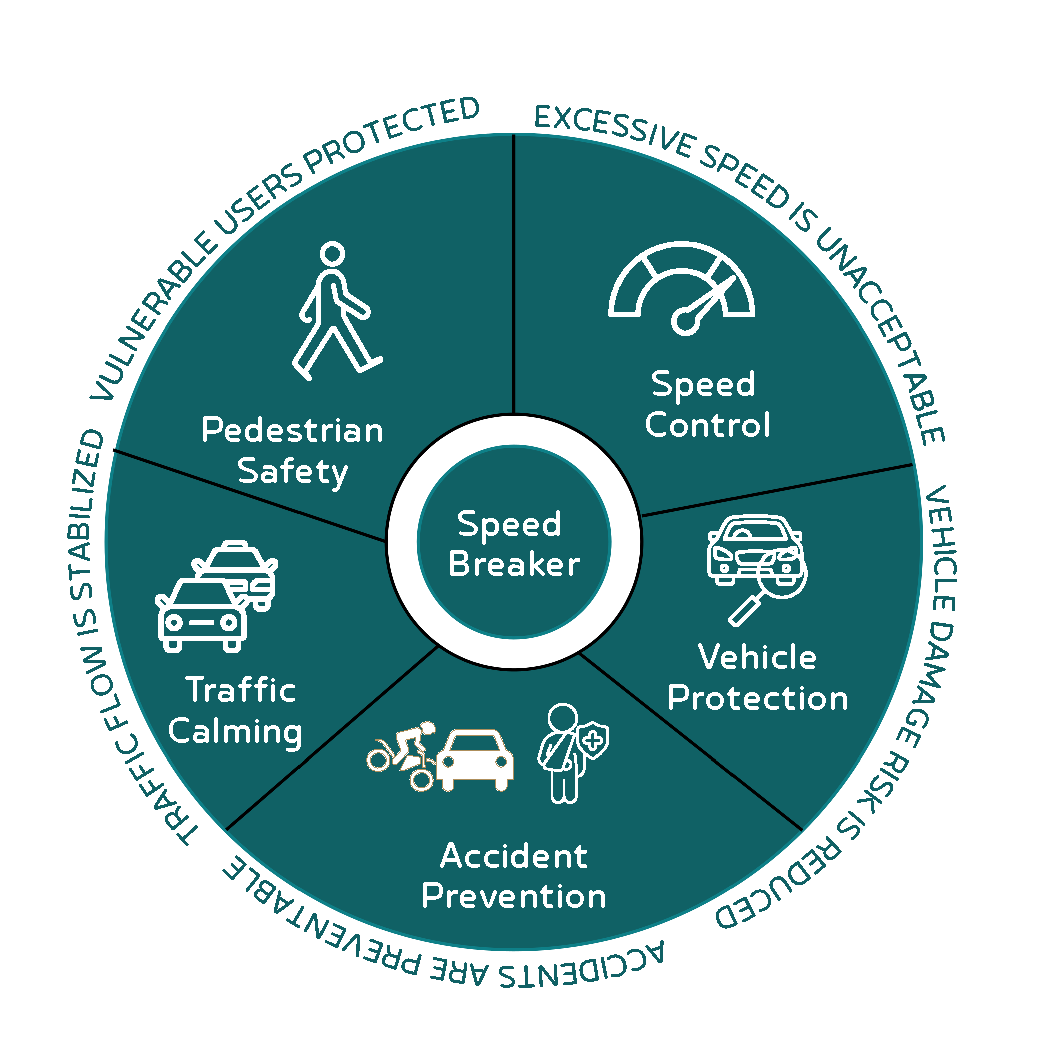
\includegraphics[width=0.7\textwidth]{Images/CH_6/6.1.pdf}
    % Figure 6.1 placeholder
    \caption{Multidimensional safety impact of speed breakers as traffic calming infrastructure, revealing their simultaneous contribution to pedestrian protection, speed enforcement, vehicular safety, and accident reduction in urban environments.}
    \label{fig:6.1}
\end{figure}

\subsection{FHWA Based Design Standards and Device Classification}

The geometric dimensions of traffic calming devices significantly influence vehicle dynamic response. To ensure practical applicability and compliance with established guidelines, the device specifications are selected according to the Federal Highway Administration (FHWA) Traffic Calming E-Primer recommendations.

Three commonly used device types are considered:

\textbf{(1) Speed Bump}

Speed bumps are designed for strict speed enforcement in low speed environments such as parking lots and private roads. These devices typically have heights up to 6 inches and short lengths ranging from 1 to 3 feet. Due to their abrupt elevation change, they induce significant vertical excitation and require very low traversal speeds.

\textbf{(2) Speed Hump}

Speed humps are intended for residential streets where moderate speed reduction is required. They typically measure 3 to 4 inches in height over a length of approximately 12 feet. Compared to speed bumps, their elongated profile reduces vertical acceleration and pitch excitation while maintaining speed control effectiveness.

\textbf{(3) Speed Table}

Speed tables incorporate extended profiles with heights of 3 to 4 inches and lengths up to 20 feet. These devices include a flat top region and are often used at pedestrian crossings and intersections. Their longer geometry produces smoother suspension response and reduced pitch oscillation.

The dimensional comparison of the three devices is summarized in Table 6.2.

\begin{table}[h]
\centering
\caption{Dimensional Specifications of Traffic Calming Devices.}
\label{tab:6.2}
\begin{tabular}{|l|l|l|}
\hline
\textbf{Device} & \textbf{Height $\times$ Length} & \textbf{Functional Application} \\
\hline
Speed bump  & up to 6 in $\times$ 1--3 ft & Parking facilities and private roads \\
Speed hump  & 3--4 in $\times$ 12 ft      & Residential streets \\
Speed table & 3--4 in $\times$ 20 ft      & Pedestrian priority areas \\
\hline
\end{tabular}
\end{table}

These standardized dimensions ensure predictable dynamic behavior and enable comparative evaluation under consistent simulation conditions.

\subsection{Raised Cosine Elevation Modeling and Implementation}

To achieve a smooth and dynamically stable traffic calming profile, the vertical geometry of the speed breakers is modeled using a raised cosine function. This formulation is selected because it provides continuous slope transitions at the entry and exit of the device, thereby minimizing abrupt suspension excitation and reducing sharp variations in vertical acceleration. Unlike triangular or trapezoidal profiles, the raised cosine curve eliminates slope discontinuities and produces a more controlled dynamic response during vehicle traversal.

The resulting elevation profiles for the three device types of speed bump, speed hump, and speed table are shown in Figure \ref{fig:6.2}. The figure illustrates the variation in height and longitudinal span for each configuration while maintaining the same smooth cosine based curvature. It can be observed that the speed bump has the shortest longitudinal length and steepest curvature, leading to sharper elevation change. In contrast, the speed table exhibits a longer and more gradual profile, which distributes vertical displacement over a larger distance and reduces dynamic excitation. The speed hump represents an intermediate configuration between these two extremes.

\begin{figure}[h]
    \centering
    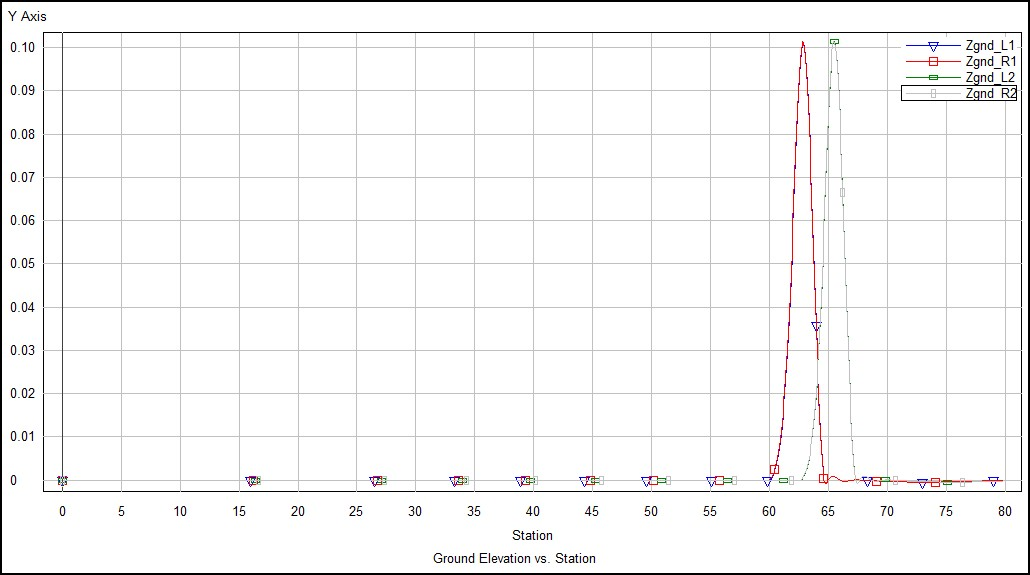
\includegraphics[width=0.7\textwidth]{Images/CH_6/6.2.jpeg}
    % Figure 6.2 placeholder
    \caption{Ground elevation profiles (Zgnd) along the path for speed hump geometry, illustrating elevation
variations experienced by front wheels (blue and red curves) and rear wheels (green and gray curves) during vehicle traversal.}
    \label{fig:6.2}
\end{figure}

\begin{figure}[h]
    \centering
    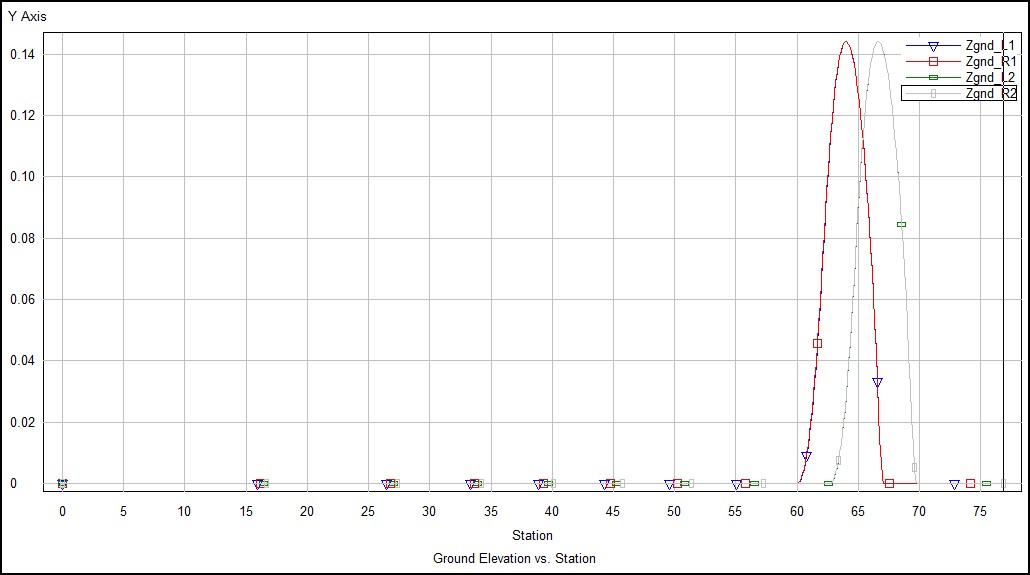
\includegraphics[width=0.7\textwidth]{Images/CH_6/6.3.jpeg}
    % Figure 6.3 placeholder
    \caption{Ground elevation profiles (Zgnd) along the path for speed hump geometry, illustrating elevation
variations experienced by front wheels (blue and red curves) and rear wheels (green and gray curves) during vehicle traversal.}
    \label{fig:6.3}
\end{figure}

The geometric parameters corresponding to these profiles are summarized in Table 6.3. These values are directly implemented in the simulation environment to ensure compliance with FHWA dimensional recommendations and to maintain consistency with the configurations evaluated in the journal study.

The analytical elevation function is discretized into station elevation pairs for numerical implementation within the CarSim road modeling interface. This discretization preserves the smoothness of the continuous profile while allowing accurate integration into the co simulation framework.

\begin{table}[h]
\centering
\caption{Discretized Station Elevation Profiles for Different Speed Breaker Types.}
\resizebox{\textwidth}{!}{
\label{tab:6.4}
\begin{tabular}{|cc|cc|cc|}
\hline
\multicolumn{2}{|c|}{\textbf{Speed Bump}} & \multicolumn{2}{c|}{\textbf{Speed Hump}} & \multicolumn{2}{c|}{\textbf{Speed Table}} \\
\hline
\textbf{Station (m)} & \textbf{Elevation (m)} & \textbf{Station (m)} & \textbf{Elevation (m)} & \textbf{Station (m)} & \textbf{Elevation (m)} \\
\hline
61.0856 & 0.0000 & 61.0000 & 0.0000 & 61.0000 & 0.0000 \\
61.3142 & 0.0762 & 61.9144 & 0.0508 & 61.7620 & 0.0508 \\
61.5428 & 0.1524 & 62.8288 & 0.1016 & 62.5240 & 0.1016 \\
61.7714 & 0.0762 & 63.7432 & 0.0508 & 65.5720 & 0.1016 \\
62.0000 & 0.0000 & 64.6576 & 0.0000 & 66.3340 & 0.0508 \\
        &        &         &        & 67.0960 & 0.0000 \\
\hline
\end{tabular}}
\end{table}

The complete workflow for converting the analytical raised cosine formulation into a simulation ready road profile is illustrated in Figure \ref{fig:6.4}. This workflow demonstrates the sequential process of defining geometric parameters, generating the elevation curve, discretizing the data, and importing the profile into the CarSim environment for dynamic evaluation.

\begin{figure}[h]
    \centering
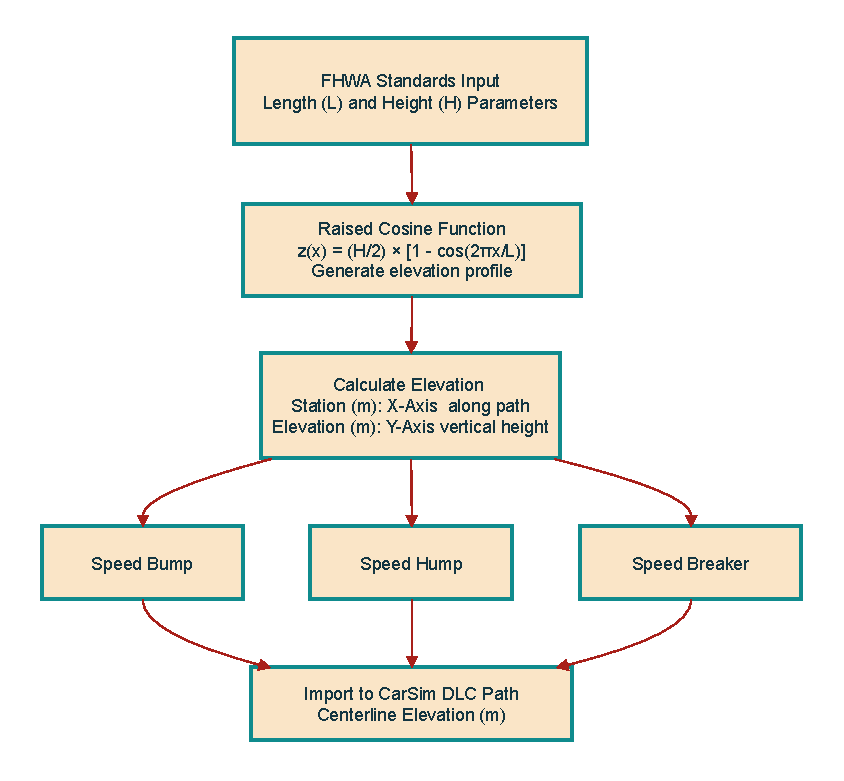
\includegraphics[width=0.7\textwidth]{Images/CH_6/6.4.pdf}
    % Figure 6.4 placeholder
    \caption{Workflow for generating and importing raised cosine speed breaker profiles into the CarSim MATLAB co simulation environment.}
    \label{fig:6.4}
\end{figure}

By embedding the discretized raised cosine profile within the double lane change scenario, the vehicle dynamic response can be evaluated under combined lateral and vertical excitation conditions. This integrated approach ensures that the geometric design is assessed not only for static shape compliance but also for its dynamic influence on ride comfort metrics.

\subsection{Safe Speed Formulation}

The dynamic response induced during speed breaker traversal depends not only on geometric shape but also on traversal velocity. Although the raised cosine profile ensures smooth slope continuity, excessive vehicle speed significantly amplifies vertical acceleration. Since ride comfort is directly influenced by acceleration magnitude, it is necessary to establish an analytical relationship between device geometry and induced vertical acceleration. This relationship enables determination of a traversal speed that maintains acceleration within acceptable comfort limits.

The vertical elevation profile is defined as:

\begin{equation}
z(s) = \frac{H}{2}\left( 1 - \cos\left( \frac{\pi(s - S_{0})}{L} \right) \right) \tag{6.6}
\end{equation}

Assuming constant longitudinal speed $V$, the spatial coordinate is expressed in the time domain as:

\begin{equation}
s(t) = S_{0} + Vt \tag{6.7}
\end{equation}

Substituting into the elevation equation yields the time dependent vertical displacement:

\begin{equation}
z(t) = \frac{H}{2}\left( 1 - \cos\left( \frac{\pi Vt}{L} \right) \right) \tag{6.8}
\end{equation}

The first derivative with respect to time provides vertical velocity:

\begin{equation}
\dot{z}(t) = \frac{H}{2}\left( \frac{\pi V}{L} \right)\sin\left( \frac{\pi Vt}{L} \right) \tag{6.9}
\end{equation}

Differentiating again gives vertical acceleration:

\begin{equation}
\ddot{z}(t) = \frac{H}{2}\left( \frac{\pi V}{L} \right)^{2}\cos\left( \frac{\pi Vt}{L} \right) \tag{6.10}
\end{equation}

The maximum vertical acceleration occurs when the cosine term equals unity, resulting in:

\begin{equation}
a_{z,\max} = \frac{H}{2}\left( \frac{\pi V}{L} \right)^{2} \tag{6.11}
\end{equation}

Equation (6.11) indicates that peak acceleration increases proportionally with device height and the square of traversal speed, and decreases with increasing device length.

To ensure ride comfort compliance, the maximum acceleration is constrained to an allowable threshold $a_{\lim}$. By equating the peak acceleration to this limit and solving for velocity, the safe traversal speed is obtained as:

\begin{equation}
V_{s} = \sqrt{\frac{2a_{\lim}L^{2}}{H\pi^{2}}} \tag{6.12}
\end{equation}

This expression defines the geometry dependent safe speed used for adaptive longitudinal regulation during speed breaker traversal.

\subsection{Adaptive Longitudinal Control Strategy}

The geometry dependent safe traversal speed derived in the previous subsection provides the allowable velocity limit required to maintain vertical acceleration within acceptable ride comfort thresholds. However, practical enforcement of this speed constraint requires a closed loop longitudinal control mechanism capable of dynamically adjusting vehicle torque during speed breaker interaction. For this purpose, an adaptive longitudinal control strategy is implemented within the CarSim--MATLAB co simulation framework.

The overall control architecture, illustrated in Figure \ref{fig:6.5}, integrates the high fidelity vehicle dynamics model in CarSim with a fuzzy logic \cite{zadeh1988fuzzy} based torque controller developed in MATLAB/Simulink. During simulation, vehicle states including longitudinal velocity and positional information are continuously transmitted from CarSim to the controller block. The controller evaluates the deviation between the current vehicle speed and the allowable safe speed determined from the geometric acceleration constraint. Based on this deviation, a torque command is generated and fed back into the vehicle model, forming a closed loop regulation system.

\begin{figure}[h]
    \centering
     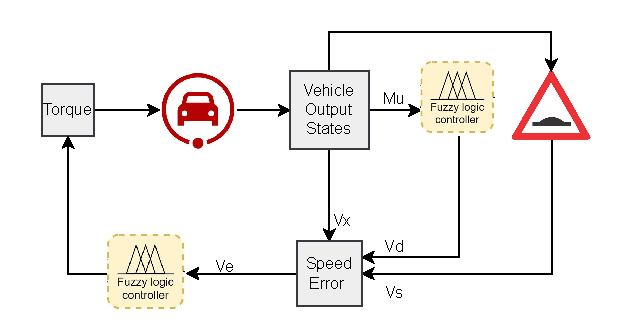
\includegraphics[width=0.8\textwidth]{Images/CH_6/6.5.pdf}
    % Figure 6.5 placeholder
    \caption{Block diagram of the control system, showing torque input regulated through vehicle output states and speed error feedback.}
    \label{fig:6.5}
\end{figure}

As the vehicle approaches the speed breaker, the controller gradually reduces the driving torque to ensure smooth deceleration toward the computed safe speed. During traversal, the torque is modulated to maintain velocity within the allowable limit, preventing excessive vertical acceleration and pitch excitation. After the vehicle exits the speed breaker, torque is progressively increased to restore the desired cruising speed without introducing abrupt acceleration that could destabilize the vehicle during the double lane change maneuver.

The fuzzy control structure ensures smooth and continuous torque variation, avoiding discontinuities associated with conventional switching based control methods. This adaptive speed regulation mechanism establishes a direct link between analytical geometry based speed constraints and practical longitudinal control implementation, thereby enabling coordinated management of ride comfort and dynamic stability during combined lateral and vertical excitation.

\section{Simulation Results and Discussion}

\subsection{Scenario Description}

The performance of the proposed raised cosine speed breaker framework is evaluated using a CarSim--MATLAB/Simulink co simulation environment. The test configuration consists of a double lane change (DLC) maneuver \cite{lee2018verification} with an embedded raised cosine speed breaker to introduce combined lateral and vertical excitation. The layout of the DLC maneuver with the integrated speed breaker is shown in Figure \ref{fig:6.6}.

\begin{figure}[h]
    \centering
     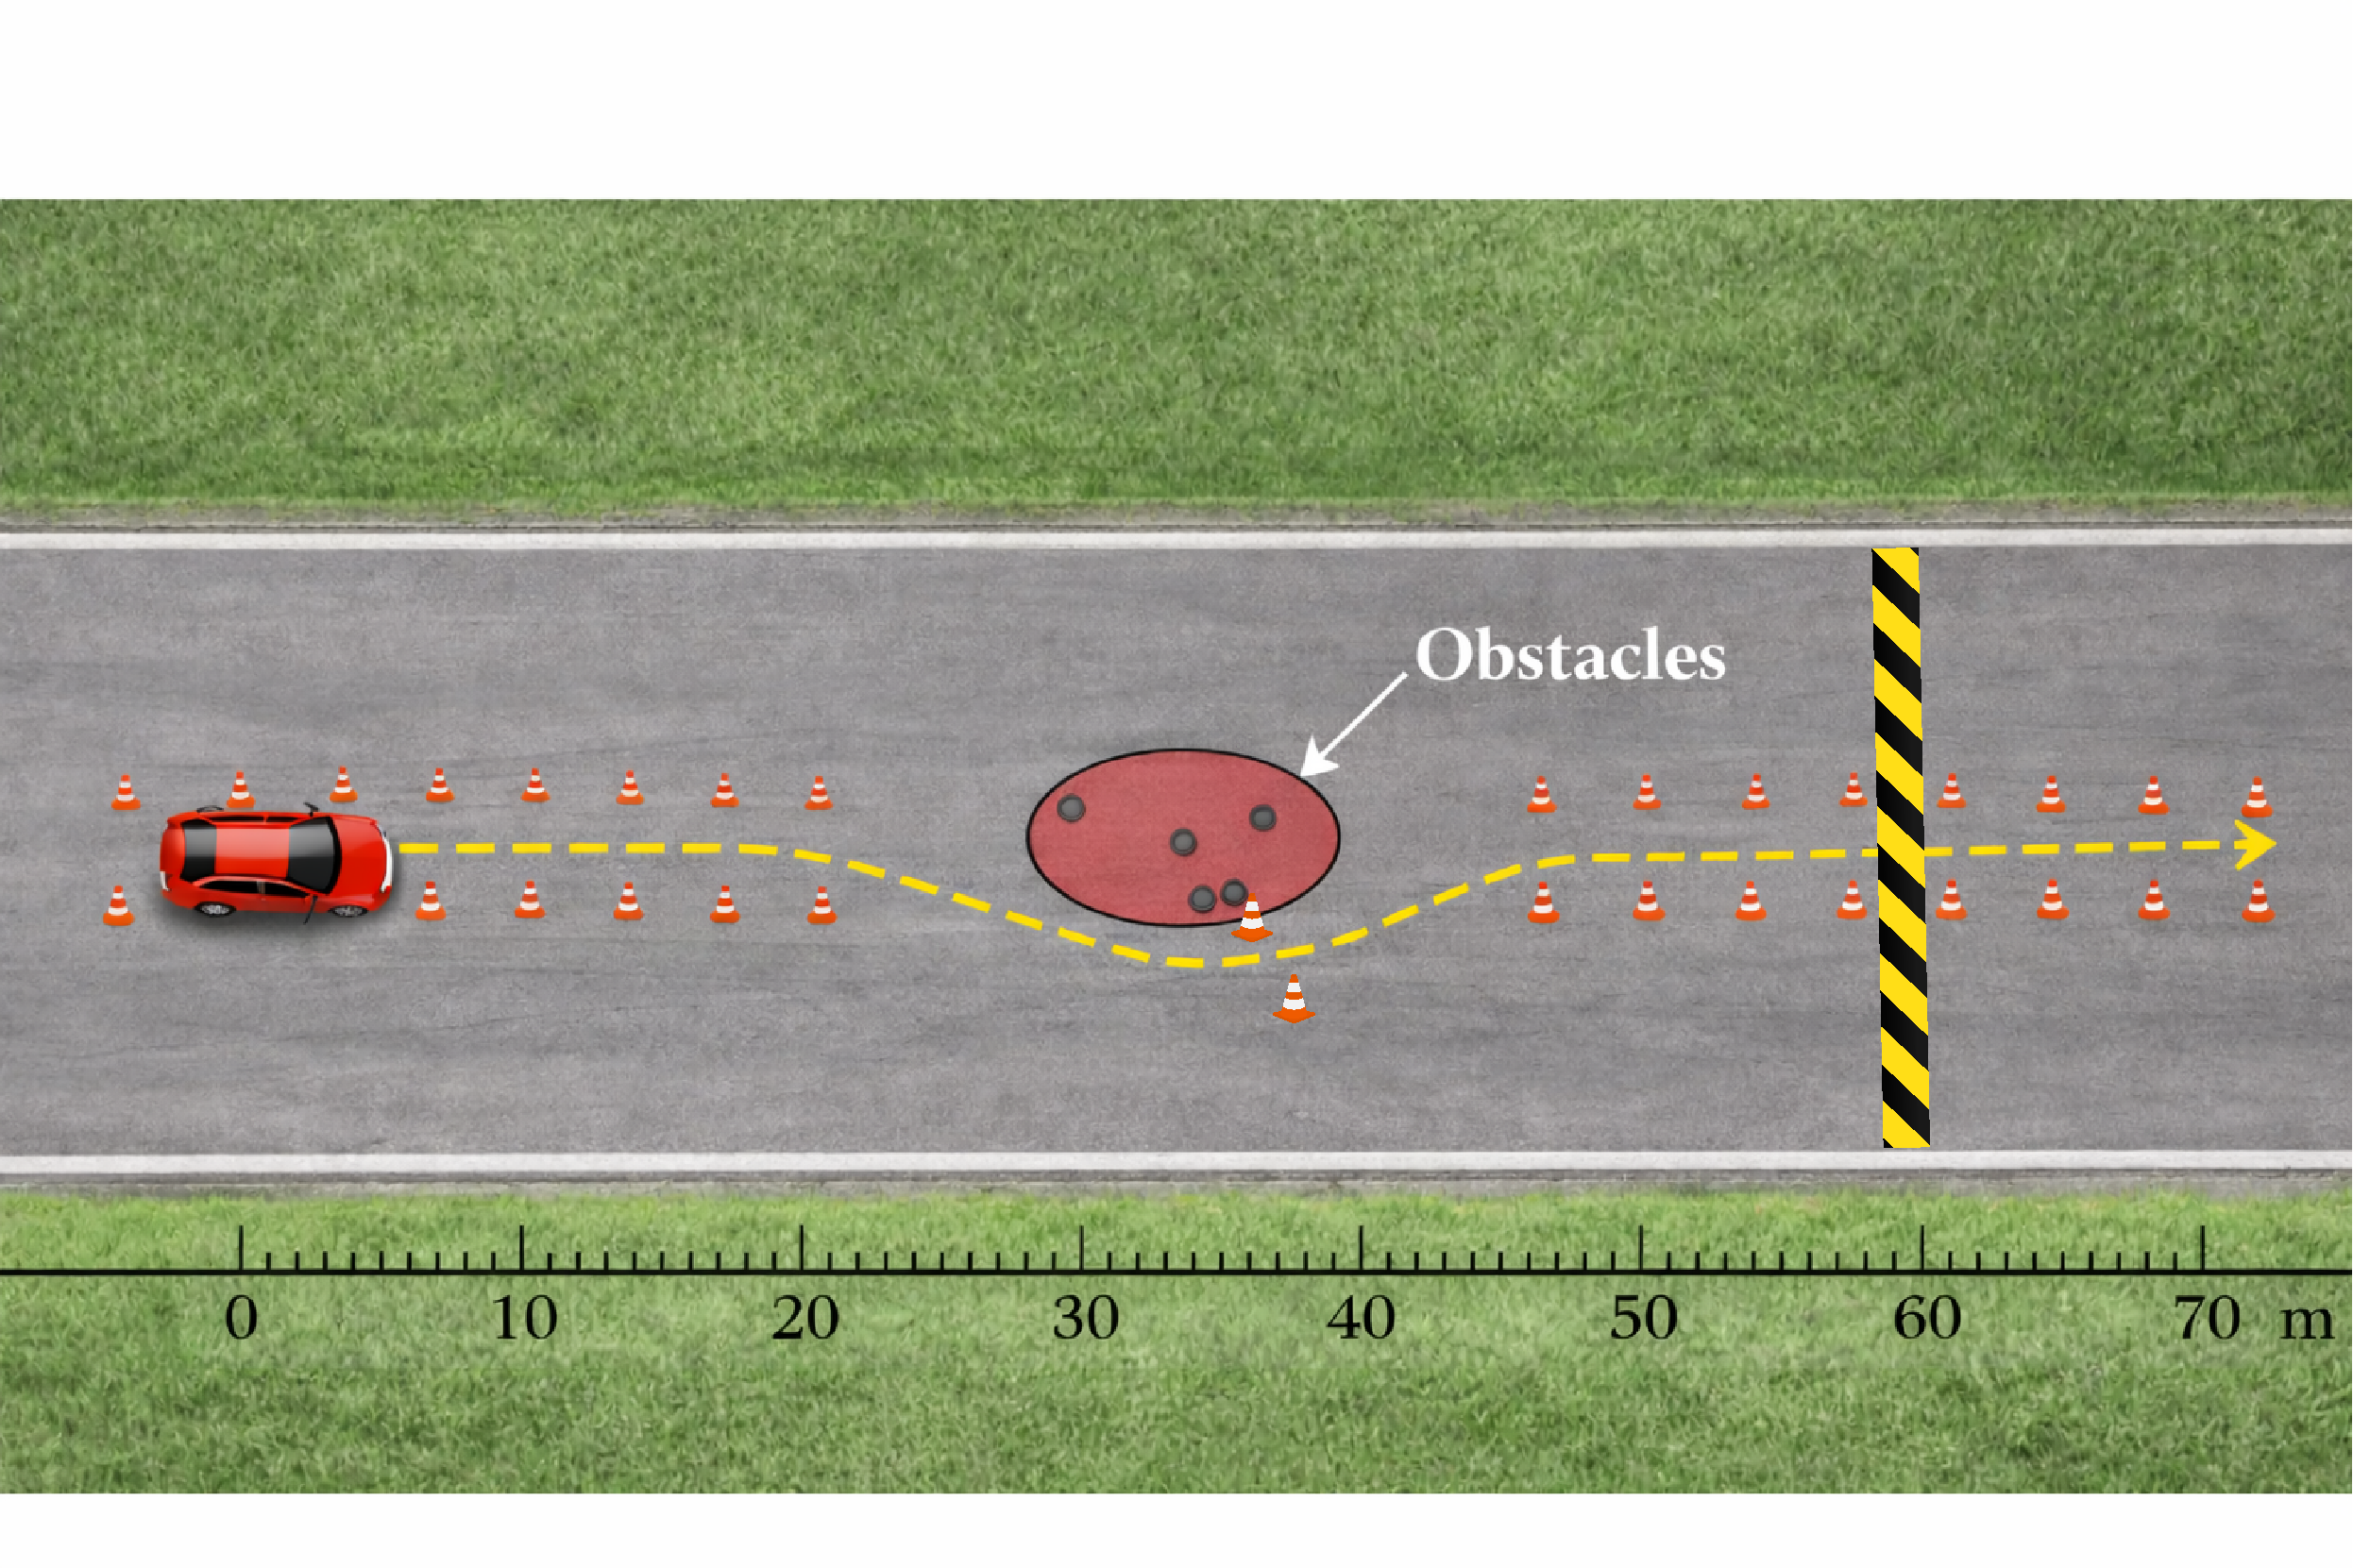
\includegraphics[width=0.7\textwidth]{Images/CH_6/6.6.pdf}
    % Figure 6.6 placeholder
    \caption{Test setup in CarSim showing a 70-meter Double Lane Change maneuver with an integrated speed breaker, illustrating
the vehicle’s initial position and the prescribed trajectory (yellow dots) for combined lane change and traffic calming assessment.}
    \label{fig:6.6}
\end{figure}

The vehicle approaches the speed breaker at an initial speed of 50 km/h under dry road friction conditions. Three traffic calming devices are evaluated: speed bump, speed hump, and speed table, each modeled using the raised cosine geometry described previously. For each configuration, the geometry dependent safe speed is applied through the adaptive longitudinal control strategy.

The proposed framework is compared with a baseline configuration without geometry based speed regulation. The evaluation focuses on vertical acceleration, pitch motion, velocity response, and traversal time during speed breaker crossing.

\subsection{Vertical Acceleration Analysis}

The vertical acceleration response is evaluated individually for each traffic calming device in order to examine the influence of geometric profile and adaptive speed regulation on ride comfort performance.

For the \textbf{speed bump}, the vertical acceleration response is presented in Figure \ref{fig:6.7}. Due to its short longitudinal length and relatively steep elevation profile, the baseline configuration produces a sharp acceleration peak when the vehicle traverses the device at the initial approach speed. The abrupt curvature results in rapid suspension compression and rebound, leading to higher acceleration magnitude. After applying the geometry dependent speed regulation strategy, the peak acceleration is significantly reduced. The reduction occurs because the traversal speed is lowered according to the analytically derived safe speed, which directly limits the acceleration term proportional to the square of velocity. This demonstrates that for short and steep devices such as speed bumps, speed regulation plays a dominant role in controlling vertical excitation.

\begin{figure}[h]
    \centering
     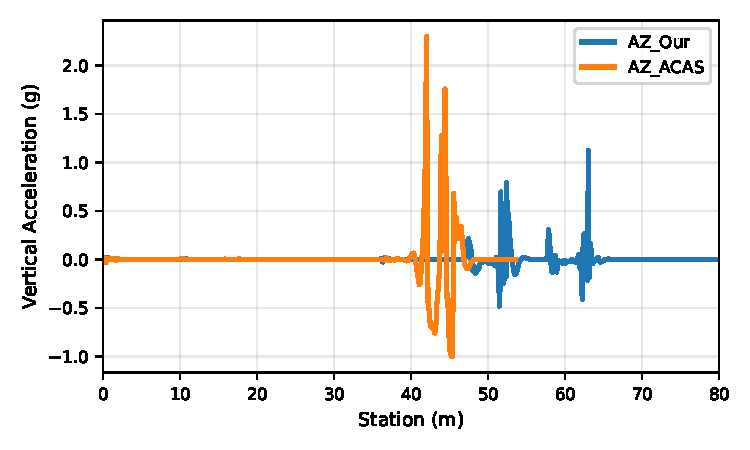
\includegraphics[width=0.6\textwidth]{Images/CH_6/6.7.pdf}
    % Figure 6.7 placeholder
    \caption{Vertical acceleration response for speed bump under baseline and adaptive speed control conditions.}
    \label{fig:6.7}
\end{figure}

For the \textbf{speed hump}, the corresponding acceleration response is shown in Figure \ref{fig:6.8}. Compared to the speed bump, the baseline acceleration peak is inherently lower due to the longer profile length, which distributes vertical displacement over a greater distance. The smoother curvature reduces abrupt suspension movement. With adaptive speed control, a further reduction in peak acceleration is observed. However, the percentage improvement is comparatively smaller than that of the speed bump because the hump geometry already provides moderate smoothness. The results confirm that geometric elongation reduces dynamic excitation even before speed regulation is applied, while adaptive control further enhances ride comfort.

\begin{figure}[h]
    \centering
    % Figure 6.8 placeholder
     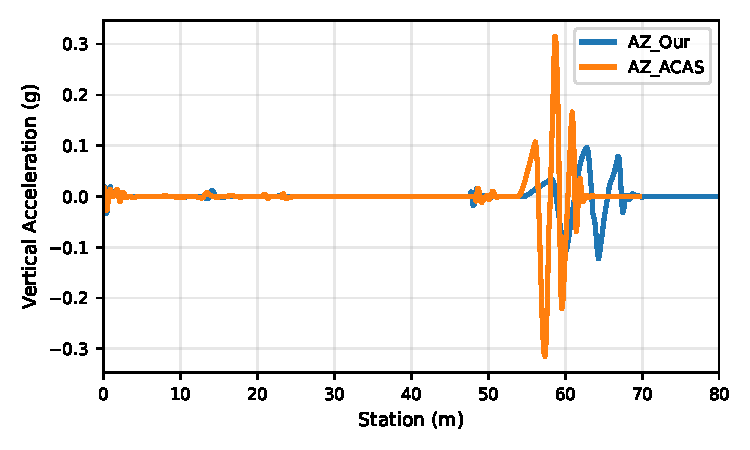
\includegraphics[width=0.7\textwidth]{Images/CH_6/6.8.pdf}
    \caption{Vertical acceleration response for speed hump under baseline and adaptive speed control conditions.}
    \label{fig:6.8}
\end{figure}

For the \textbf{speed table}, the acceleration response is illustrated in Figure \ref{fig:6.9}. The extended longitudinal length and gradual elevation transition produce the lowest baseline acceleration among the three devices. The longer flat top region allows the vehicle to traverse with minimal abrupt vertical displacement. When adaptive speed regulation is applied, the acceleration profile becomes even smoother, with reduced peak magnitude and less pronounced oscillatory behavior. Although the absolute reduction in acceleration is smaller compared to the speed bump case, the combined effect of elongated geometry and controlled speed results in the most comfortable traversal condition.

\begin{figure}[h]
    \centering
     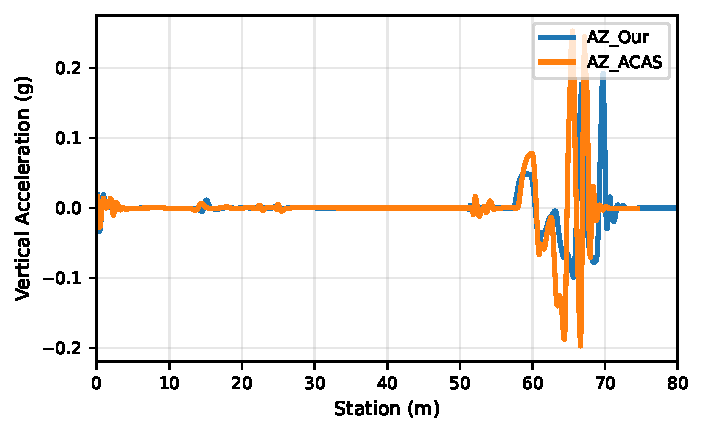
\includegraphics[width=0.6\textwidth]{Images/CH_6/6.9.pdf}
    % Figure 6.9 placeholder
    \caption{Vertical acceleration response for speed table under baseline and adaptive speed control conditions.}
    \label{fig:6.9}
\end{figure}

The comparative results indicate that vertical acceleration is strongly influenced by both geometric parameters and traversal speed. Shorter and steeper profiles generate higher dynamic excitation, whereas longer profiles inherently reduce acceleration amplitude. The adaptive speed regulation framework effectively limits acceleration magnitude across all configurations, with the most substantial improvement observed for the speed bump case.

\subsection{Pitch Motion Analysis}

Pitch motion \cite{bindschadel2022active} represents the rotational behavior of the vehicle body about the lateral axis during speed breaker traversal. It directly influences ride comfort, longitudinal load transfer, and vehicle stability during transient maneuvers. The fundamental pitch states experienced during traversal are illustrated in Figure \ref{fig:6.10}.

\begin{figure}[h]
    \centering
     
\includegraphics[width=0.7\textwidth]{Images/CH_6/6.10.pdf}
    % Figure 6.10 placeholder
    \caption{Illustration of pitch states during speed breaker traversal, no pitch motion, negative pitch (pitch down), and positive pitch (pitch up).}
    \label{fig:6.10}
\end{figure}

As shown in Figure \ref{fig:6.10}, when the front axle encounters the elevated profile, the vehicle undergoes positive pitch rotation (nose up motion). Conversely, when the rear axle passes over the device, a negative pitch response (nose down motion) occurs. The magnitude of these rotations depends on the rate of vertical displacement and suspension dynamics. In the absence of elevation disturbance, the vehicle maintains a near zero pitch angle, representing stable longitudinal equilibrium.

The rotational axes used for evaluating pitch dynamics are illustrated in Figure \ref{fig:6.11}.

\begin{figure}[h]
    \centering
     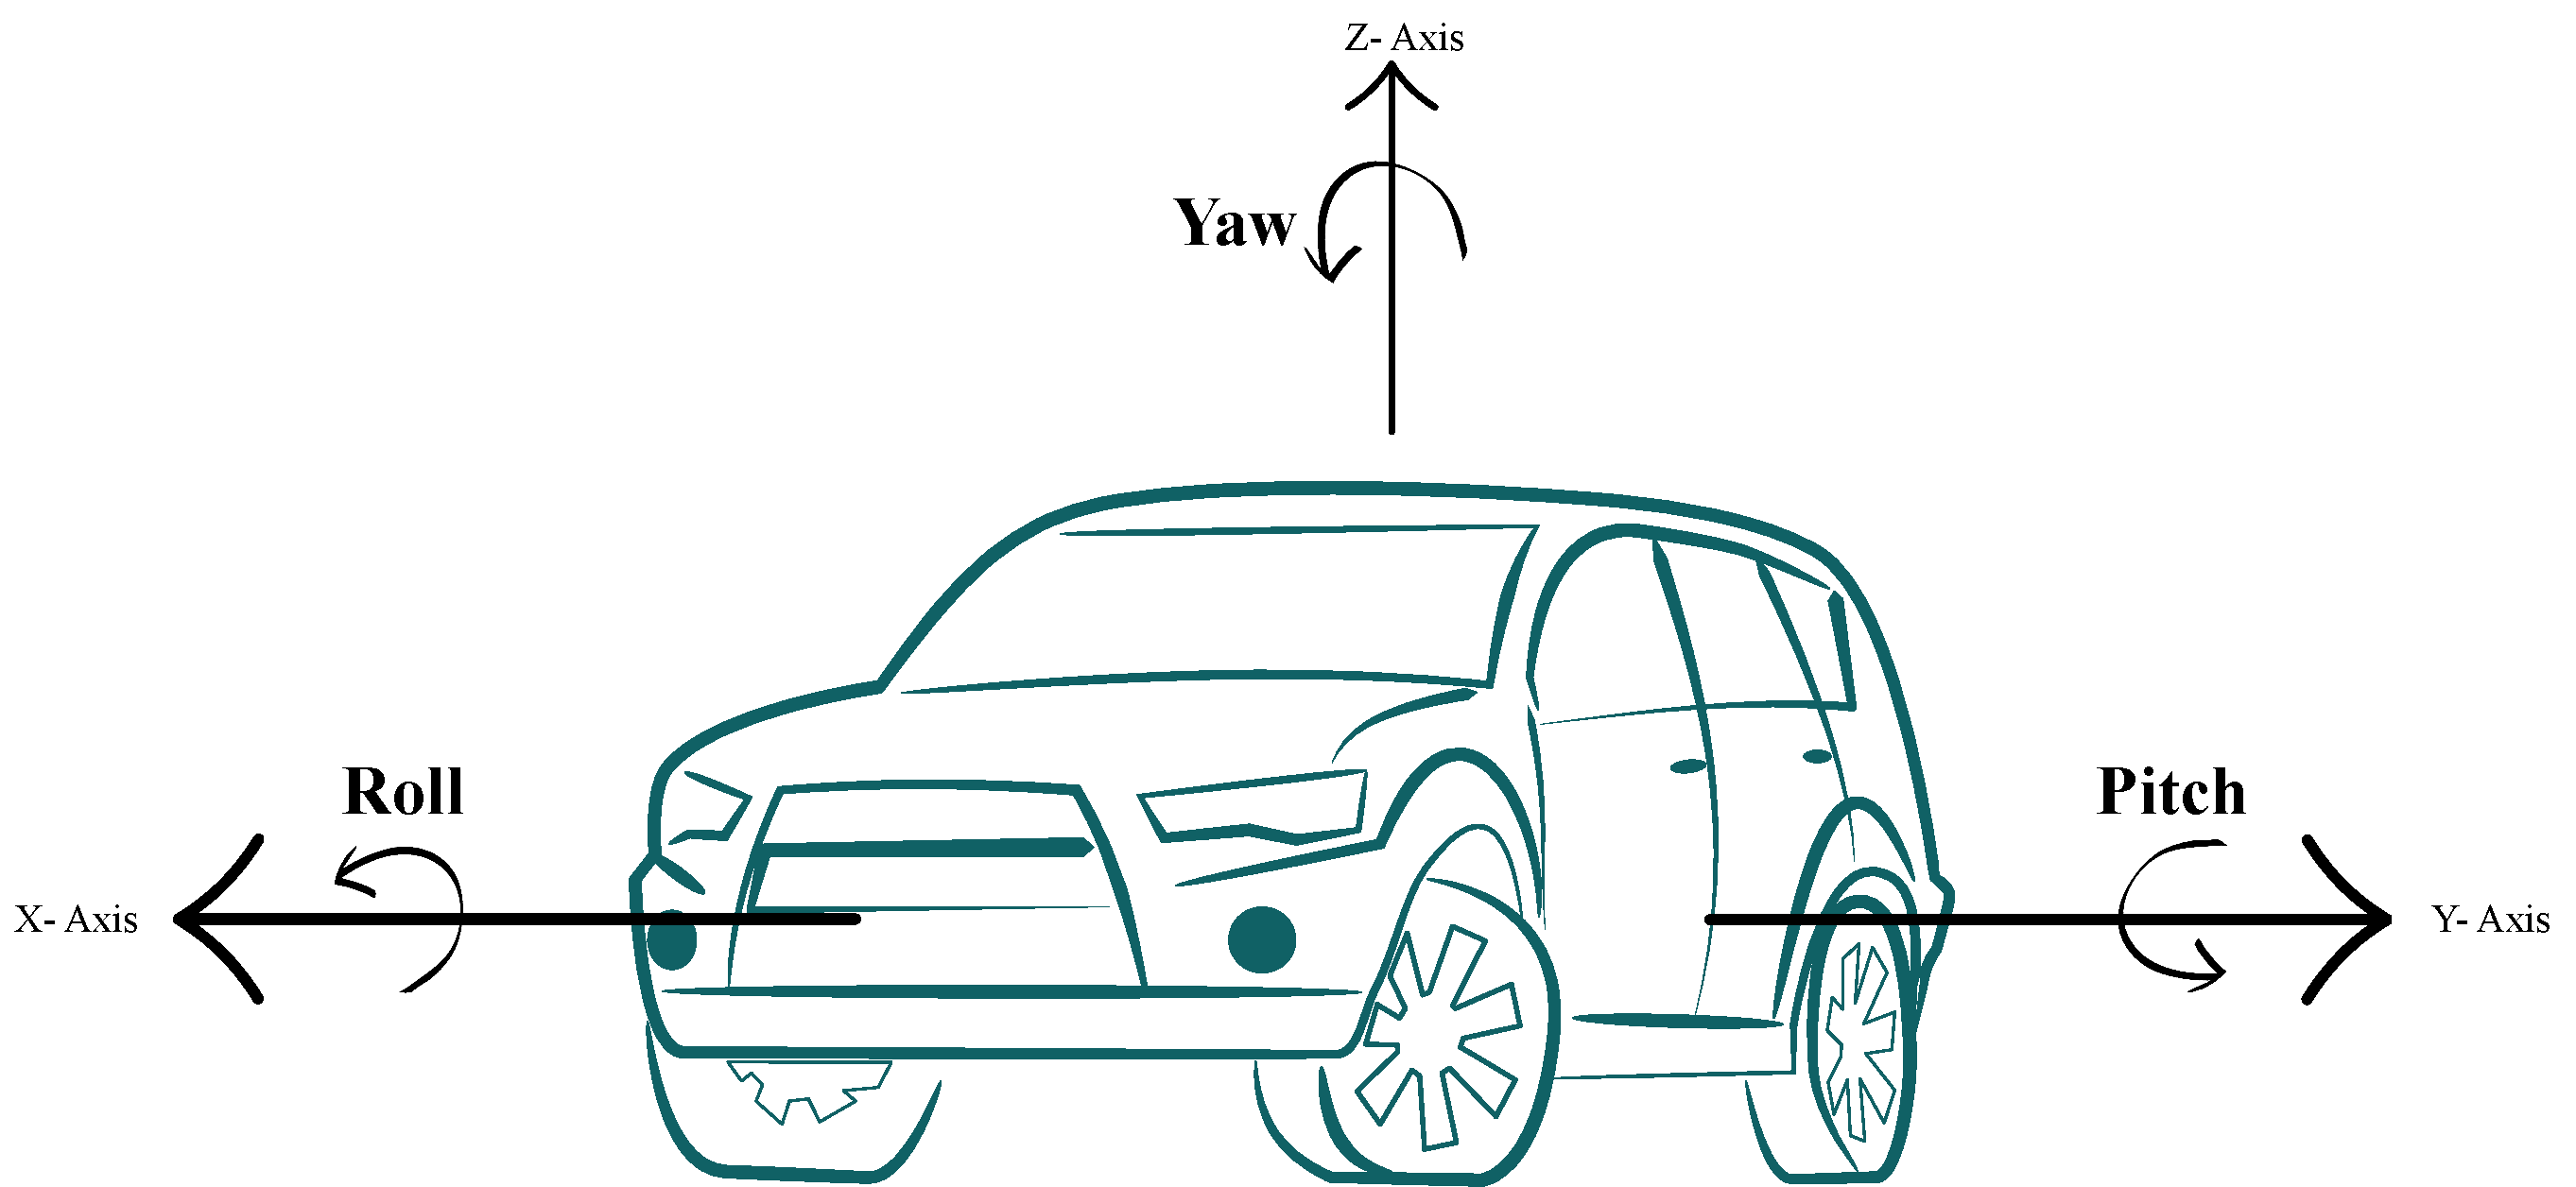
\includegraphics[width=0.7\textwidth]{Images/CH_6/6.11.pdf}
    % Figure 6.11 placeholder
    \caption{Representation of vehicle rotational degrees of freedom with corresponding axis: yaw (rotation about Z-axis), roll(rotation about X-axis), and pitch (rotation about Y-axis) used in vehicle dynamics analysis.}
    \label{fig:6.11}
\end{figure}

Figure \ref{fig:6.11} defines pitch rotation about the lateral axis, distinct from roll and yaw motions. During speed breaker traversal, pitch motion dominates the rotational response because vertical displacement occurs sequentially at the front and rear axles. Therefore, pitch angle serves as a primary indicator of rotational comfort and dynamic stability.

The pitch angle response for the \textbf{speed bump} configuration is presented in Figure \ref{fig:6.12}. The baseline ACAS system exhibits a pronounced pitch peak due to the abrupt elevation transition of the short bump geometry. The rapid front axle lift induces a sharp positive pitch spike, followed by a significant negative oscillation as the rear axle crosses the device. In contrast, the proposed adaptive speed regulation method reduces both peak magnitude and oscillatory amplitude. The reduced traversal speed lowers the rate of vertical excitation, resulting in smoother rotational transition and faster stabilization after exit.

\begin{figure}[h]
    \centering
     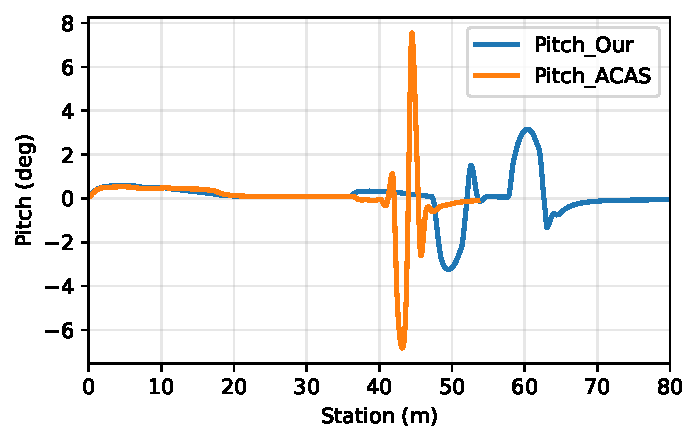
\includegraphics[width=0.6\textwidth]{Images/CH_6/6.12.pdf}
    % Figure 6.12 placeholder
    \caption{Pitch angle response for speed bump, comparison between proposed method and ACAS system.}
    \label{fig:6.12}
\end{figure}

For the \textbf{speed hump}, the pitch response is shown in Figure \ref{fig:6.13}. Compared to the speed bump, the hump geometry produces a lower baseline pitch amplitude due to its longer profile and smoother curvature. The ACAS configuration still shows noticeable rotational oscillation; however, the magnitude is smaller than that observed in the bump case. The proposed method further suppresses peak pitch angle and shortens the settling time. The smoother rotational transition indicates improved dynamic balance between front and rear suspension excitation.

\begin{figure}[h]
    \centering
     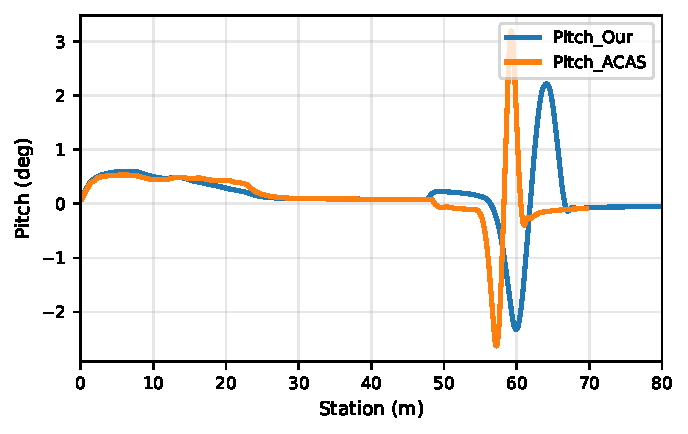
\includegraphics[width=0.6\textwidth]{Images/CH_6/6.13.pdf}
    % Figure 6.13 placeholder
    \caption{Pitch angle response for speed hump, comparison between proposed method and ACAS system.}
    \label{fig:6.13}
\end{figure}

The pitch response for the \textbf{speed table} is illustrated in Figure \ref{fig:6.14}. Owing to its extended longitudinal length and flat top region, the speed table produces the smallest baseline pitch variation among the three devices. The ACAS response exhibits moderate rotational deviation, while the proposed framework achieves further reduction in peak angle and oscillatory behavior. The longer traversal duration distributes vertical displacement more gradually, resulting in reduced rotational impulse and improved body stability.

\begin{figure}[h]
    \centering
    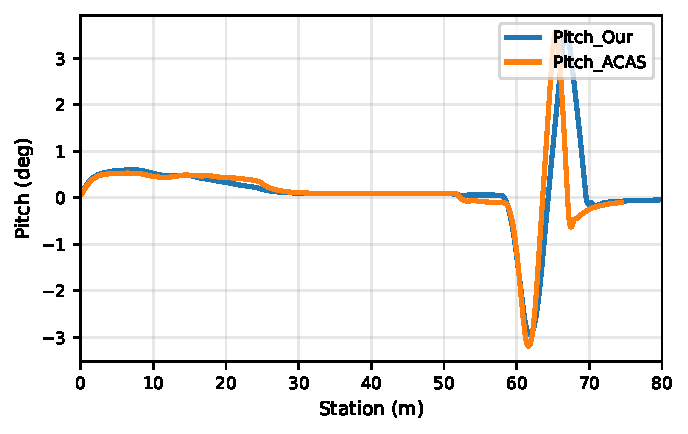
\includegraphics[width=0.6\textwidth]{Images/CH_6/6.14.pdf}
    % Figure 6.14 placeholder
    \caption{Pitch angle response for speed table, comparison between proposed method and ACAS system.}
    \label{fig:6.14}
\end{figure}

Overall, the pitch motion analysis demonstrates that rotational excitation is strongly dependent on geometric abruptness and traversal speed. Shorter devices generate larger pitch peaks due to rapid front rear axle elevation differences, whereas elongated geometries inherently reduce rotational impulse. The adaptive speed regulation strategy consistently decreases peak pitch magnitude and improves settling behavior across all configurations, confirming its effectiveness in enhancing ride comfort under combined longitudinal and lateral excitation.

\subsection{Velocity Response Analysis}

The longitudinal velocity response is examined separately for each traffic calming device in order to evaluate the enforcement of the geometry dependent safe speed and its influence on dynamic behavior.

For the \textbf{speed bump}, the velocity profile is presented in Figure \ref{fig:6.15}. Under the ACAS configuration, the vehicle approaches and crosses the bump at a nearly constant speed, resulting in limited pre emptive deceleration. This behavior contributes to the higher vertical acceleration and pronounced pitch peaks observed previously. In contrast, the proposed method exhibits a controlled reduction in speed before reaching the bump. The velocity decreases smoothly to align with the computed safe speed and remains regulated during traversal. After crossing, the speed is gradually restored without abrupt acceleration. This controlled velocity transition directly explains the significant reduction in acceleration and pitch magnitude for the bump case.

\begin{figure}[h]
    \centering
    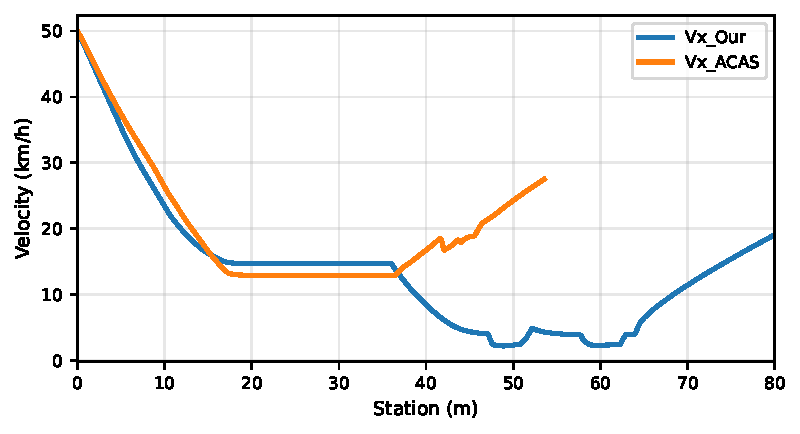
\includegraphics[width=0.7\textwidth]{Images/CH_6/6.15.pdf}
    % Figure 6.15 placeholder
    \caption{Longitudinal velocity response for speed bump, comparison between proposed method and ACAS system.}
    \label{fig:6.15}
\end{figure}

For the \textbf{speed hump}, the velocity response is shown in Figure \ref{fig:6.16}. The ACAS configuration maintains a relatively steady approach speed, with only minor variations during traversal. Because the hump geometry is smoother than the bump, the dynamic impact is inherently lower; however, the absence of geometry dependent regulation still permits higher excitation compared to the proposed framework. The adaptive method demonstrates moderate deceleration prior to the hump, aligning vehicle speed with the allowable limit. The speed variation is smoother and more gradual compared to the bump case, reflecting the less aggressive geometry. This controlled profile contributes to improved pitch stability and reduced vertical acceleration.

\begin{figure}[h]
    \centering
     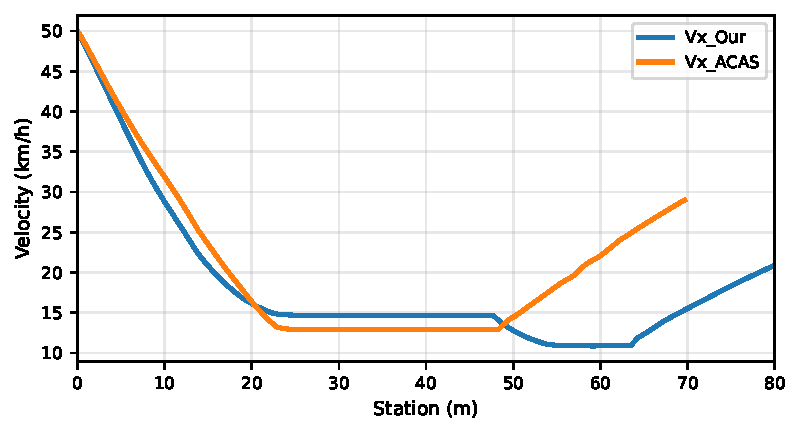
\includegraphics[width=0.6\textwidth]{Images/CH_6/6.16.pdf}
    % Figure 6.16 placeholder
    \caption{Longitudinal velocity response for speed hump, comparison between proposed method and ACAS system.}
    \label{fig:6.16}
\end{figure}

For the \textbf{speed table}, the velocity response is illustrated in Figure \ref{fig:6.17}. Due to its extended longitudinal length, the baseline ACAS response shows minimal speed fluctuation during traversal. The proposed method introduces a slight but controlled deceleration before entering the elevated section, ensuring compliance with the calculated safe speed. The speed remains stable throughout the flat top region and is smoothly increased after exit. The difference between the two methods is less pronounced than in the bump case, reflecting the inherently smoother geometry of the speed table. Nevertheless, the regulated speed profile enhances overall dynamic smoothness and contributes to improved ride comfort.

\begin{figure}[h]
    \centering
    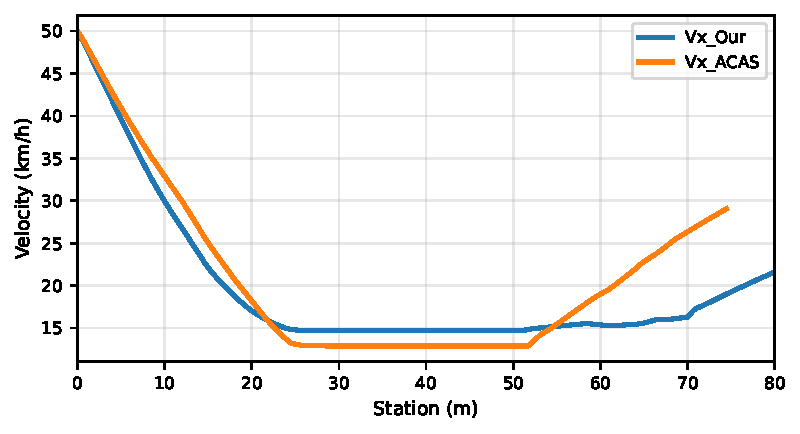
\includegraphics[width=0.6\textwidth]{Images/CH_6/6.17.pdf}
    % Figure 6.17 placeholder
    \caption{Longitudinal velocity response for speed table, comparison between proposed method and ACAS system.}
    \label{fig:6.17}
\end{figure}

The velocity analysis confirms that the adaptive speed regulation strategy effectively enforces geometry dependent speed limits across all device types. The most substantial speed reduction occurs for the speed bump, where geometric abruptness necessitates stricter velocity control. For the hump and table configurations, the speed adjustments are comparatively moderate, corresponding to their smoother profiles. Regulated velocity behavior directly supports the reductions in vertical acceleration and pitch motion observed in the preceding sections.

\subsection{Traversal Time Comparison}

The traversal time over each traffic calming device is evaluated to examine the trade off between ride comfort enhancement and operational efficiency. While the proposed adaptive speed regulation reduces vertical acceleration and pitch motion, it is important to assess whether this improvement introduces excessive delay during traversal. The crossing duration for each device type under both the ACAS configuration and the proposed method is presented in Figure \ref{fig:6.18}.

\begin{figure}[h]
    \centering
    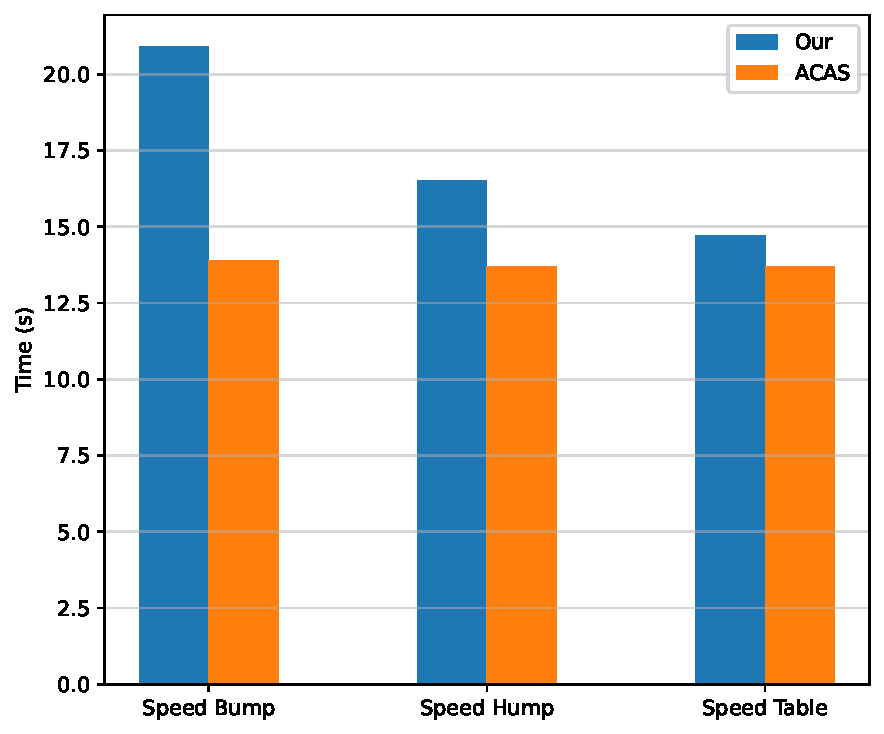
\includegraphics[width=0.7\textwidth]{Images/CH_6/6.18.pdf}
    % Figure 6.18 placeholder
    \caption{Traversal time comparison for speed bump, speed hump, and speed table profiles under proposed and ACAS configurations, with crossing duration presented in seconds.}
    \label{fig:6.18}
\end{figure}

For the \textbf{speed bump}, the adaptive regulation strategy results in a noticeable increase in traversal time compared to the ACAS configuration. This is expected, as the short and steep geometry requires significant speed reduction to satisfy acceleration constraints. Although the crossing duration increases slightly, the improvement in ride comfort and reduction in dynamic excitation justify the trade off.

For the \textbf{speed hump}, the increase in traversal time is moderate. Because the hump geometry is smoother and allows higher safe speed compared to the bump, the required deceleration is less aggressive. Consequently, the time penalty remains limited while still achieving measurable comfort improvement.

For the \textbf{speed table}, the difference in traversal time between the two methods is minimal. The elongated geometry inherently permits relatively stable traversal, and only minor speed adjustment is required under the proposed framework. As a result, the impact on operational efficiency is negligible.

Overall, the traversal time analysis demonstrates that the adaptive speed regulation framework improves ride comfort with only a modest increase in crossing duration. The most significant time variation occurs for the speed bump, which corresponds to the largest reduction in vertical and pitch excitation. For smoother geometries, the comfort gain is achieved with minimal influence on traversal efficiency.

\subsection{Comparative Performance Evaluation}

The combined results of vertical acceleration, pitch motion, velocity response, and traversal time provide a comprehensive assessment of the proposed ride comfort oriented framework. Across all traffic calming configurations, the adaptive speed regulation strategy consistently improves dynamic performance compared to the ACAS baseline system.

For the \textbf{speed bump} \cite{pau2001speed}, which represents the most abrupt geometry, the proposed method yields the largest reduction in peak vertical acceleration and pitch amplitude. The controlled deceleration prior to traversal significantly limits dynamic excitation generated by the short and steep elevation profile. Although this improvement introduces a moderate increase in traversal time, the enhancement in ride comfort and reduction in oscillatory behavior demonstrate a favorable trade off.

For the \textbf{speed hump} \cite{yeo2020effects}, the smoother and elongated geometry inherently reduces dynamic severity compared to the bump. The adaptive speed regulation further stabilizes vehicle motion by moderating longitudinal velocity before and during crossing. The resulting improvements in acceleration and pitch response are noticeable, while the increase in traversal time remains limited.

For the \textbf{speed table} \cite{moreno2011speed}, the extended longitudinal length produces the lowest baseline dynamic disturbance. The proposed framework refines the already smooth response by reducing minor oscillations and stabilizing pitch motion, with minimal impact on crossing duration. This confirms that the effectiveness of speed regulation is proportional to geometric abruptness: the shorter and steeper the device, the greater the benefit of adaptive control.

Overall, the results establish a clear relationship between geometric profile, traversal speed, and vehicle dynamic response. The raised cosine formulation provides smooth elevation continuity, while the geometry dependent speed regulation effectively constrains acceleration magnitude. The integration of analytical speed derivation with adaptive torque control ensures coordinated management of longitudinal and vertical dynamics during combined lateral maneuvering.

The comparative analysis confirms that the proposed framework achieves enhanced ride comfort without compromising vehicle stability, thereby validating the effectiveness of geometry based speed regulation in traffic calming applications.

\section{ Summary}

This chapter presented a ride comfort oriented framework for speed breaker design based on raised cosine geometry and adaptive speed regulation. The study established a direct relationship between geometric profile parameters and vehicle dynamic response, highlighting the influence of device height, longitudinal length, and traversal speed on vertical acceleration and pitch motion. A geometry dependent safe speed formulation was developed to constrain vertical acceleration within acceptable comfort limits. This analytical relationship was integrated into a closed loop longitudinal control strategy implemented in a CarSim MATLAB co simulation environment. The adaptive torque regulation mechanism ensured smooth deceleration prior to traversal, controlled speed maintenance during crossing, and gradual recovery after exit. Simulation results under a double lane change maneuver demonstrated that the proposed framework consistently reduces peak vertical acceleration and pitch oscillation across speed bump, speed hump, and speed table configurations. The most significant improvement was observed for the speed bump due to its abrupt geometry, while smoother devices exhibited moderate yet measurable enhancements. Although traversal time increased slightly in certain cases, the trade off remained acceptable relative to the achieved improvement in ride comfort and dynamic stability. Overall, the findings confirm that combining analytically derived geometric constraints with adaptive speed control provides an effective strategy for improving ride comfort performance of traffic calming devices without compromising vehicle stability. The framework establishes a systematic approach for geometry based speed regulation in urban traffic applications.
\chapter{CONCLUSION AND FUTURE WORK}

\section{Conclusion}

Autonomous driving systems are increasingly expected to operate safely and reliably under diverse and uncertain road conditions. While significant progress has been made in perception, planning, and control, many existing approaches treat these components as isolated modules and often overlook the combined influence of computational efficiency, interpretability, and passenger comfort. The objective of this research was to develop a unified framework that integrates hybrid path planning, LLM based advisory reasoning, and geometry driven ride comfort modeling into a coherent and practically viable system. To address computational limitations of classical sampling based planners, a Hybrid Adaptive A* RRT* framework was developed. The integration of heuristic guidance with probabilistic exploration enabled the planner to achieve improved convergence behavior while maintaining solution feasibility in structured and semi structured environments. Comparative evaluation demonstrated that the hybrid approach reduces unnecessary exploration, improves planning efficiency, and provides a controllable balance between path optimality and runtime performance. The influence of adaptive weighting parameters was systematically analyzed, confirming that the proposed method offers flexibility without compromising stability. Beyond geometric planning, this thesis introduced a Large Language Model based advisory layer designed to enhance interpretability and contextual reasoning within the decision making pipeline. Rather than replacing deterministic control mechanisms, the LLM module was integrated as a supervisory reasoning component that interprets driving states and provides structured, human readable explanations. Experimental analysis confirmed that this integration improves system transparency without introducing instability into the control loop. The results demonstrate that language driven reasoning can coexist with traditional planning architectures, forming a layered structure that enhances trust and debuggability in safety critical systems. In addition to navigation performance, ride comfort was addressed through a raised cosine based geometric modeling of speed breakers, including bumps, humps, and tables. Analytical modeling and simulation based validation demonstrated that properly designed geometric profiles significantly reduce peak vertical acceleration and pitch disturbances. The derived safe traversal speeds were shown to align with stability and comfort thresholds, highlighting the importance of integrating infrastructure aware modeling into vehicle control strategies. The findings confirm that comfort oriented geometry design plays a crucial role in maintaining dynamic stability during vertical disturbances. When viewed collectively, the results of this thesis establish a unified architectural contribution. The hybrid planner enhances computational efficiency, the LLM advisory layer improves interpretability, and the geometry driven analysis ensures ride comfort and stability. Rather than treating efficiency, explainability, and comfort as separate objectives, the proposed framework demonstrates that these dimensions can be integrated within a structured and analytically grounded system. Overall, this research contributes to the advancement of autonomous driving systems by presenting a balanced methodology that combines deterministic optimization, adaptive reasoning, and infrastructure aware modeling. The proposed framework provides a scalable and extensible foundation for future autonomous platforms that require not only accurate navigation but also transparency and passenger comfort.

\section{Future Work}

While the proposed framework demonstrates promising performance within a controlled simulation environment, several directions remain open for further investigation and practical deployment. First, real world validation is necessary to evaluate system robustness under physical sensor noise, actuator delays, and unpredictable environmental variations. Hardware in the loop experiments and controlled field testing would provide deeper insight into system reliability and operational constraints beyond simulation assumptions. Second, the LLM based advisory module can be further expanded toward multimodal integration. Incorporating perception aware language models capable of directly interpreting visual or sensor streams may enhance contextual reasoning and reduce reliance on manually structured prompts. Additionally, lightweight optimization of language models for embedded deployment remains an important area for investigation to ensure real time feasibility. Third, the hybrid planning framework can be extended to multi agent and highly dynamic urban scenarios. Cooperative navigation, interaction aware trajectory optimization, and uncertainty aware planning would further strengthen the adaptability of the system in dense traffic environments. Fourth, comfort modeling may be embedded directly into trajectory optimization rather than evaluated post analysis. Integrating vertical acceleration constraints and pitch stability criteria into the planner's cost function would enable comfort aware path generation in real time. Finally, broader infrastructure modeling, including varying road roughness, weather induced surface changes, and pedestrian dense environments, would enhance the generality of the framework. Extending the system to operate under heterogeneous road networks and adaptive regulatory conditions would move the research closer to practical deployment. In summary, the work presented in this thesis establishes a structured and integrated foundation for autonomous driving systems that prioritize efficiency, interpretability, and ride stability. Continued development along the identified directions will further strengthen the feasibility and scalability of such systems in real world applications.


\newpage
\addcontentsline{toc}{chapter}{Bibliography}


\bibliographystyle{plain}
\bibliography{mybib}

\end{document}